\chapter{GRIPHO: developing an Italian high-resolution hourly precipitation dataset}\label{chp:itaobs}
In order to simulate flood hazard on the scale of a small catchment, high resolution precipitation data is needed. This is because the time scale for floods in small areas can be very short, due to the limited ability of small rivers to displace the large amounts of water that can fall in a relatively brief timespan.
While model output can be easily obtained for this scope, observations provide a very important tool for validation and evaluation of the methodology. Therefore, in this thesis project, observations are used to drive some of the simulations described in the next chapter.

Most observational datasets over Italy and Europe are daily (see \cref{sec:obs_datasets} and \cref{tab:prec_obs_ita}), which implies that very rapid precipitation extremes, which often occur in a few hours, are necessarily smoothed out when upscaled to a daily time scale.
Analysing these extremes on an hourly time scale has the potential to provide better results for flood hazard analysis, especially for small catchments with a short water residence time.
For this reason, one of the objectives of this thesis work was the creation of an hourly precipitation dataset that could serve as input to CETEMPS Hydrological Model \citep[CHyM,][, see \cref{sec:chym} for details]{Tomassetti2005,Coppola2006}, the hydrological model of our choice, which is designed to easily digest hourly data as input and has been doing so operationally for quite some time at the CETEMPS Center of Excellence\footnote{\url{http://cetemps.aquila.infn.it/}}.\\
We thus developed what can be considered, as far as we know, the first hourly precipitation database over Italy using exclusively in-situ precipitation data as input. The dataset is named GRIPHO (GRidded Italian Precipitation Hourly Observations).
This chapter will outline the work undergone in analysing, cleaning, gridding and validating GRIPHO. The resulting dataset is deemed of sufficient quality to be used in this project.\\
Later in the project, GRIPHO was used for driving the CHyM model simulations (\cref{sec:chym}) and to validate the RegCM simulations (\cref{sec:experiments}).

%------------------------------------
%	ORIGINAL INPUT DATA
%------------------------------------
\section{Original input data} \label{sec:original_input_data}
The first challenge when developing such a dataset is collecting the data: not always a single national agency can provide all the necessary information. Fragmentation of data sources, different input formats and different levels of quality checks are the main problems that need to be addressed. As previously mentioned, Italy lacks a national repository for meteorological data: regional agencies each have their own station network, data collection and cleaning procedures. Retrieving and homogenising all the necessary information from all regional agencies can prove to be a difficult task.
In this case, the input data are provided by the CETEMPS Center of Excellence of the University of L'Aquila, as part of an agreement with the International Centre for Theoretical Physics.
The dataset is the result of integration between different data sources; observations from 3712 precipitation stations located in all of Italy over the period from 2001 to 2016 are collected, validated and filtrated by different algorithms and then provided as a collection of yearly time series.
Using this input data, a gridded hourly dataset was created and validated.

The input data is provided as yearly Fortran-style binary files. The time step is quarter-hourly, and the unit of measure reportedly \SI{}{\milli\metre\per\hour}. A single, separate metadata text file contains the following fields for each station:
\begin{itemize}
    \item Station number [int]
    \item Station name [char]
    \item Province [char]
    \item Municipality [char]
    \item Latitude [dbl]
    \item Longitude [dbl]
\end{itemize}
No information on station type, height, exposure or any other metadata is provided.
Due to the severe lack of metadata, correcting for gauge undercatch (see \cref{sec:gauge_undercatch}) is deemed too complex for the scope of this project.\\
Any value less than 0 is considered to be a filling value (most often, this is the case with -10, -999 and -9999).
The total size of the input database is about \SI{3.9}{\giga B} for the period 2001 to 2016.
In absence of any additional information, the first timestep of each yearly file is assumed to be at time January 1, 00:00:00 UTC, with the following timesteps separated by 15 minutes each.

\subsection{Conversion to NetCDF}\label{sec:netcdf}
The first step for making use of this data is the conversion to a more user-friendly format. NetCDF\footnote{\url{https://www.unidata.ucar.edu/software/netcdf/}} is chosen primarily due to its widespread use across all fields of climate science and to its ease of use and metadata integration. All modern programming languages offer one or more interfaces capable of reading self-describing NetCDF data. Additionally, NetCDF offers advanced options such as transparent compression and chunking, which can speed up reading and writing significantly. The latter, chunking, is a netCDF-4 feature which allows to tune a dataset for faster access along a specific dimension: this allows for two versions of the dataset to be created as separate files, one that assures very fast reads for the complete time-series of one single station, and one that optimised the reading of all station values for a single time-step. The industry-standard CF conventions \citep{Eaton2009} version 1.7 are followed for the storing of metadata inside the files, the total size of which resulted to be around \SI{650}{\mega B}.

\subsection{Station spatial and temporal availability}
\Cref{fig:stat_pos} shows the station distribution over the study area. The coverage of the Italian territory is very complete, with an average density of one station per $9\times9$ \si{\kilo\metre\squared}, which is on par with most European high resolution observational datasets \citep[see \cref{sec:obs_datasets} and][for details]{Prein2017}. The overall spatial distribution is quite uniform over the complete Italian teritory, with generally lower density over less climatologically complex areas, such as the Po Plain.\\
\Cref{fig:stat_distr_height} shows the height distribution of the dataset, with station height values extracted from the HydroSHEDS void-filled Digital Elevation Model \citep[][also see \cref{sec:DEM}]{Lehner2008, Lehner2013} at \ang{0.00083} (about \SI{90}{\metre}) resolution, as opposed to the spatial distribution of all of the Italian territory. All elevations are well represented in the dataset, except very high elevations (above \SI{3000}{\metre}), which is to be expected due to the difficulty in setting up and maintaining such stations. Such small underrepresentation of very high elevations should not impact the precipitation field in a noticeable way.

\begin{figure}
    \centering
    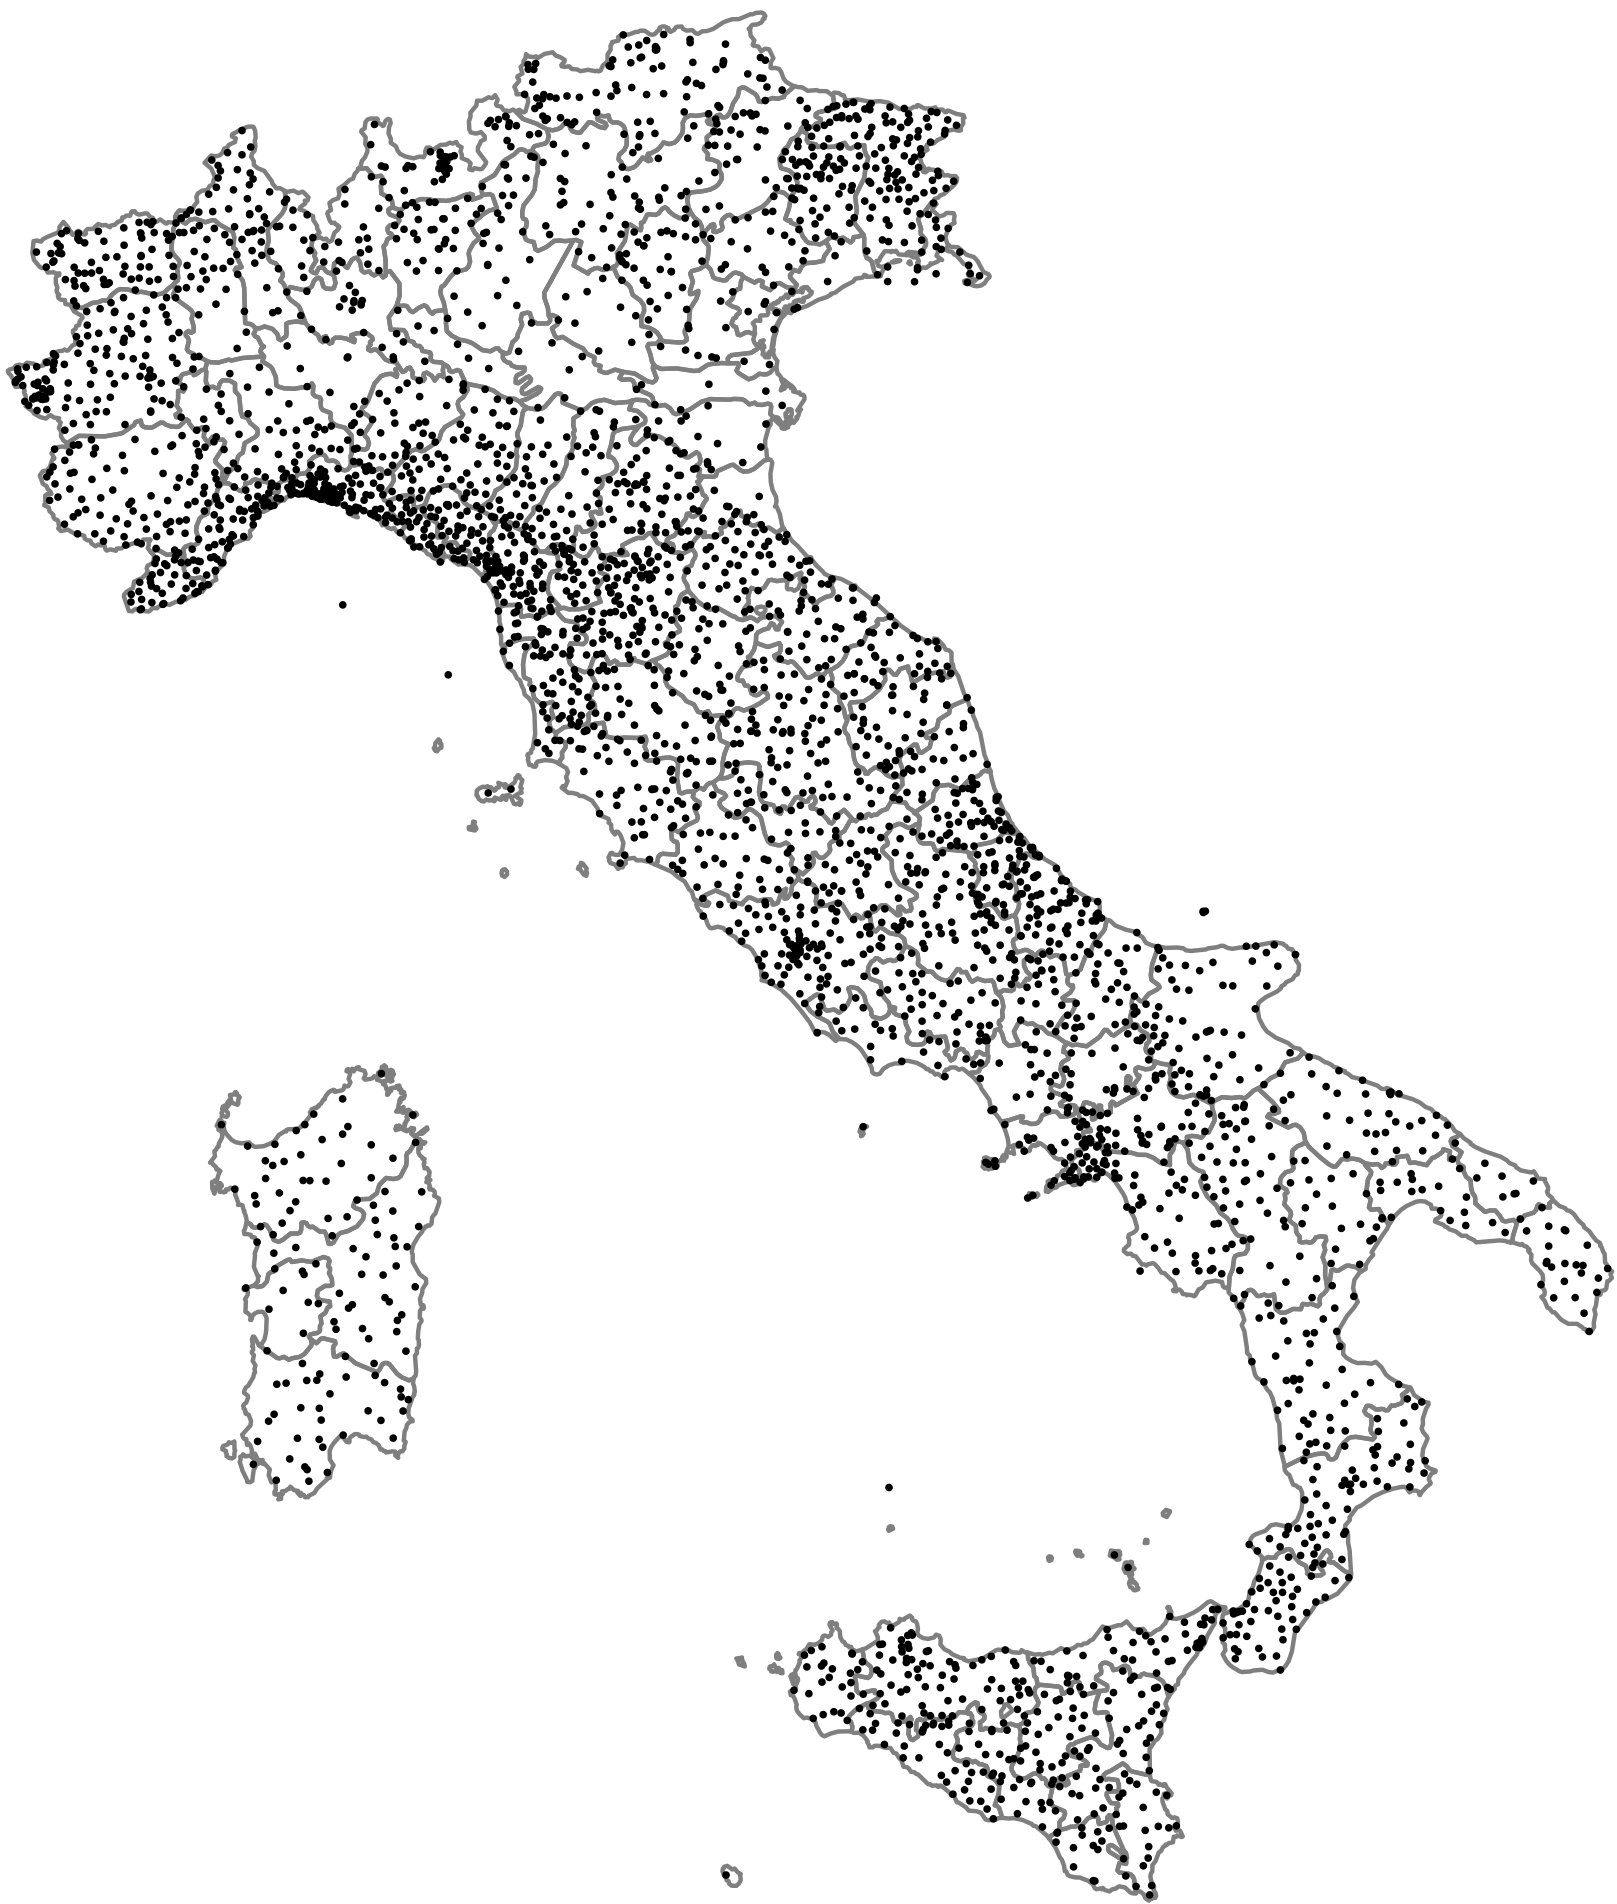
\includegraphics[width=0.7\textwidth]{figures/rain_dst/stat_pos.png}
    \decoRule
    \caption[Station spatial distribution for the Italian in-situ hourly precipitation dataset GRIPHO]{Station spatial distribution for the Italian in-situ hourly precipitation dataset. All 3712 stations in the dataset are shown, regardless of their temporal availability.}
    \label{fig:stat_pos}
\end{figure}
%here might use animate package to put a gif with one timestep for each month or year, for the final PDF

\begin{figure}
    \centering
    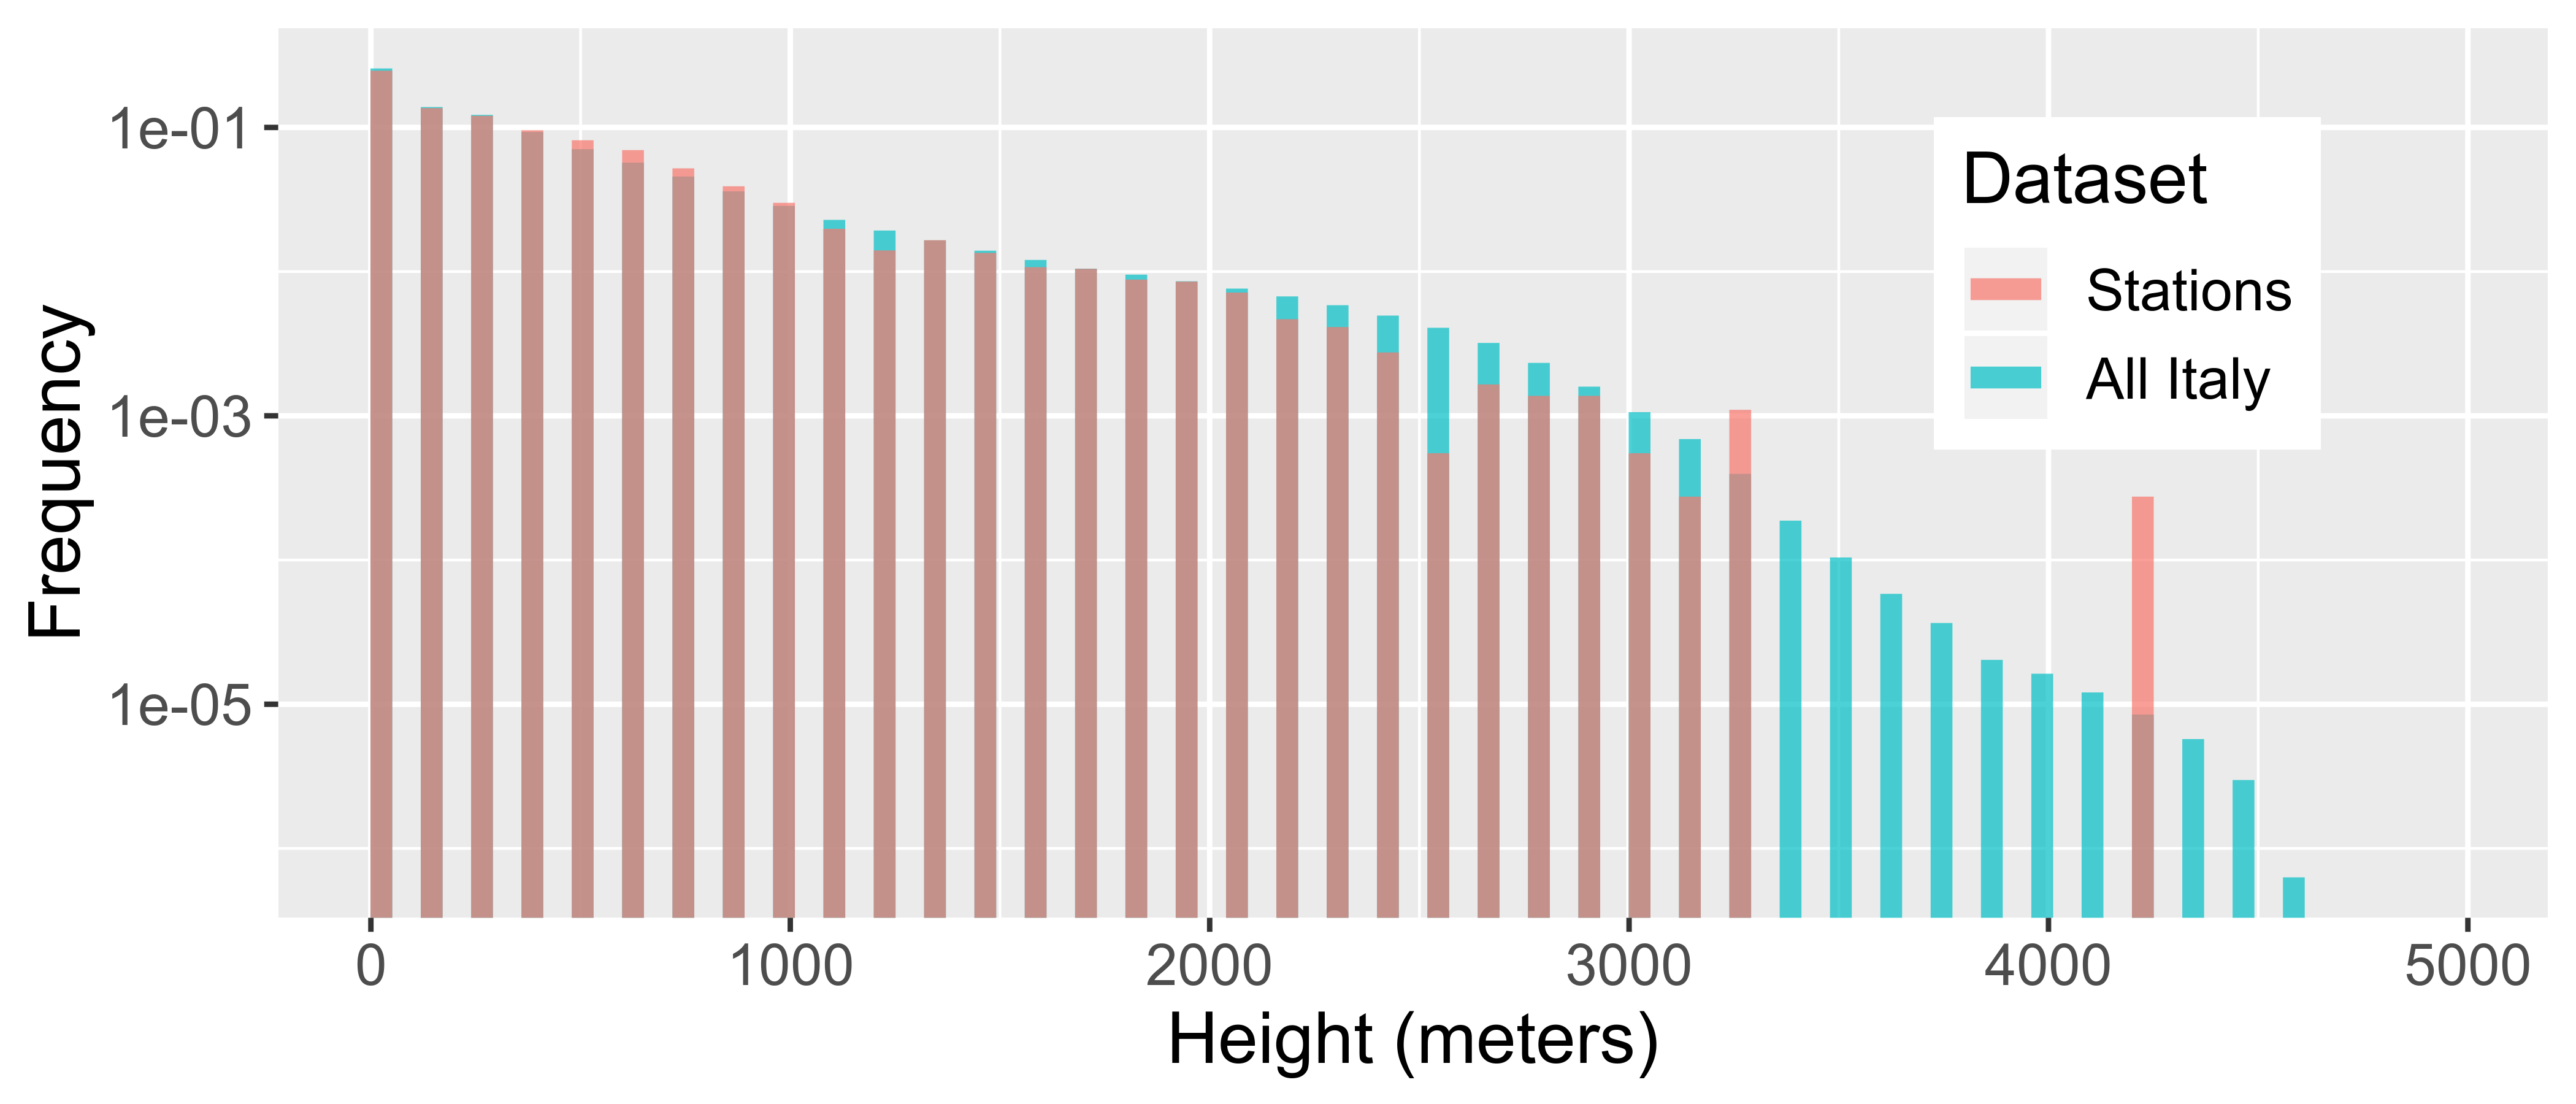
\includegraphics[width=\textwidth]{figures/rain_dst/stat_distr_height.png}
    \decoRule
    \caption[Station height distribution for the Italian in-situ hourly  precipitation dataset GRIPHO]{Station height distribution for the Italian in-situ hourly precipitation dataset (red), compared to all of the Italian territory (blue). Bin size is \SI{120}{m}. Data from the HydroSHEDS void-filled Digital Elevation Model \citep{Lehner2008, Lehner2013}.}
    \label{fig:stat_distr_height}
\end{figure}

In \cref{fig:stat_avail_ts}, the number of available stations (stations whose value is not one of the possible NaN values) is plotted over each timestep for the whole Italian territory. Station availability grows significantly within the 16-year period, which implies that the total station density is not constant. While a variable number of stations is common for all station-based datasets \citep[see for example][, figure 2]{Haylock2008}, in this case it is particularly evident, with the actual number of active stations growing from about 500 in 2001 to about 2600 in 2012. Moreover, in some timesteps (e.g. at the beginning of 2012) the number of stations falls momentarily close to zero and little to no data is reported. In order to keep the dataset as close as possible to raw station data, in the final product these voids are not filled in with alternative datasets or via interpolation, but are rather left as missing values.

\begin{figure}
    \centering
    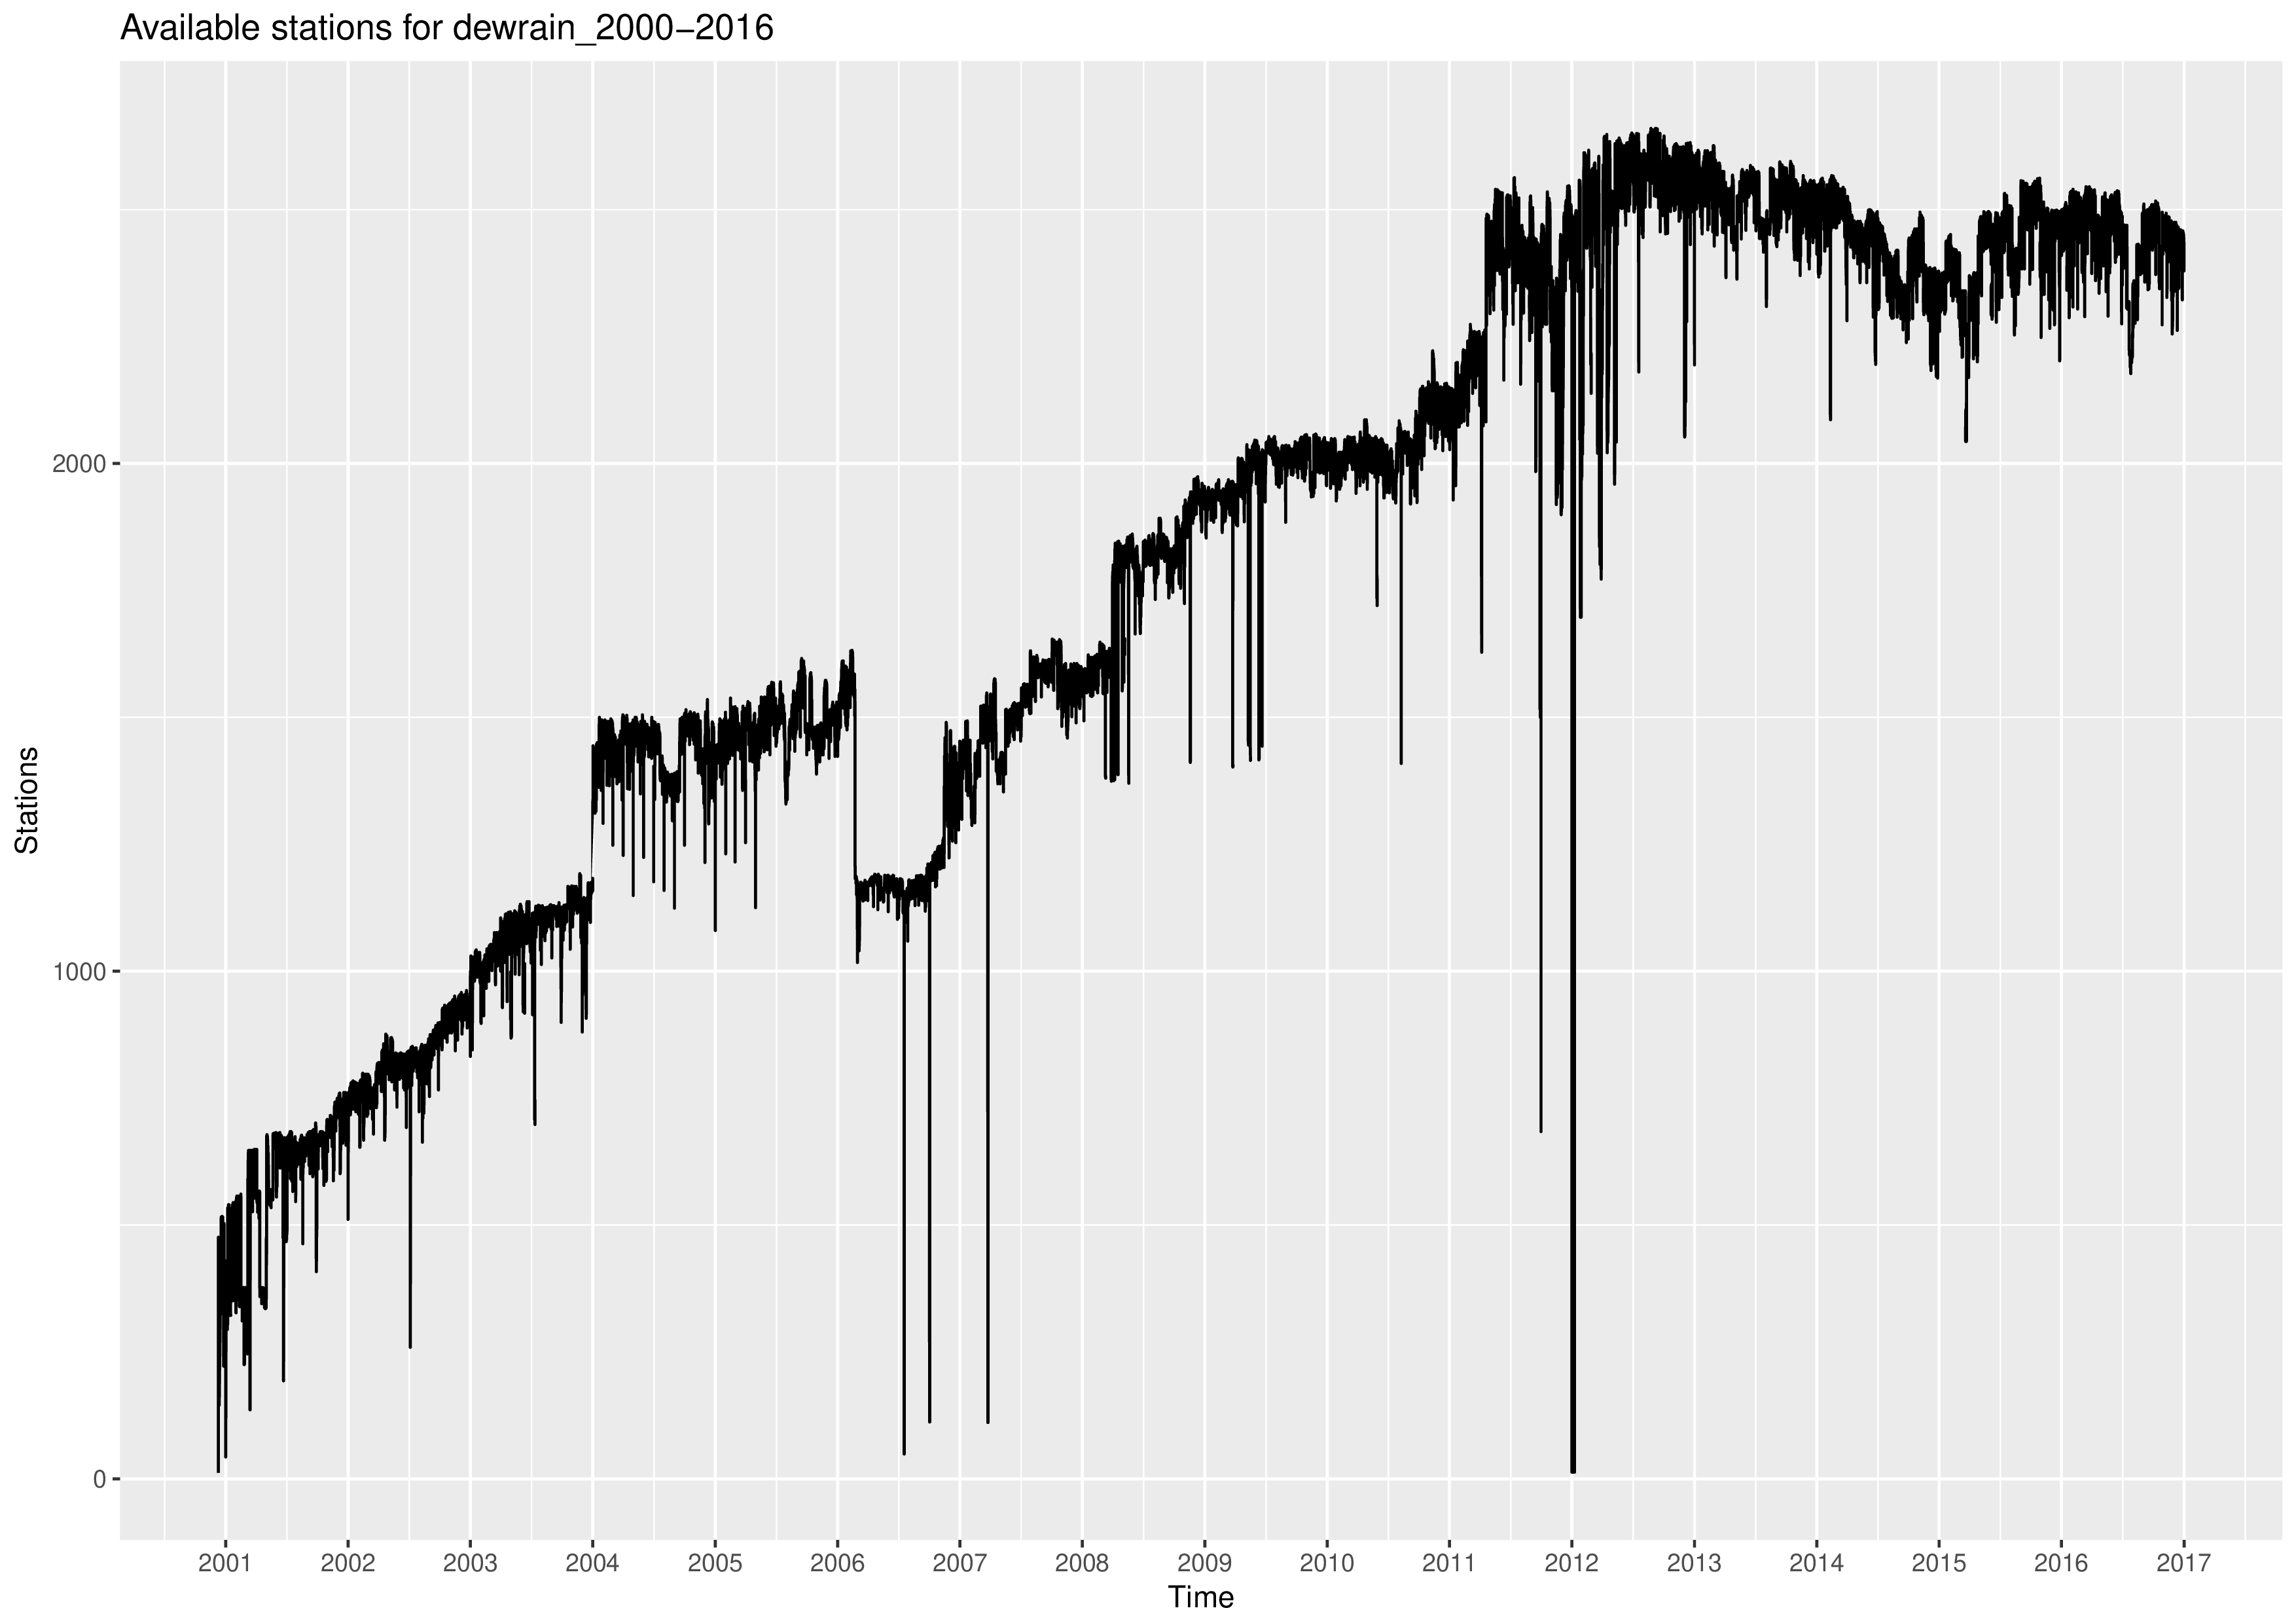
\includegraphics[width=0.7\textwidth]{figures/rain_dst/station_count_line.png}
    \decoRule
    \caption[Count of available stations per timestep]{Timeseries of the number of available stations for each timestep in the input data for the Italian in-situ dataset GRIPHO.} \label{fig:stat_avail_ts}
\end{figure}

Maps of the number of stations and valid timesteps per Italian region (\cref{fig:regional_stats}) show very low data availability for some regions, likely as a result of some regional agencies providing only a few years of data to the original data collector. While some regions provided 12 or even 13 years (Piemonte, Calabria) of data, one region (Sicily) only has 3 valid years in total (\cref{fig:regional_stats/b}). When taking into account the total number of timesteps and the station density  (\cref{fig:regional_stats/f}), Liguria and Friuli--Venezia Giulia come on top, with about \SI{2000}{valid values\per\kilo\metre\squared}, in contrast with Trentino--Alto Adige and Sicily, both with less than \SI{300}{values\per\kilo\metre\squared}. 

\begin{figure}
    \centering
    % source of this data if you want to remake it:
    % /home/afantini/places/clima-archive/flood/museodat2nc/interpolate_dewrain/valid_timesteps/
    \begin{subfigure}{.475\textwidth}
        \caption{}\label{fig:regional_stats/a}
        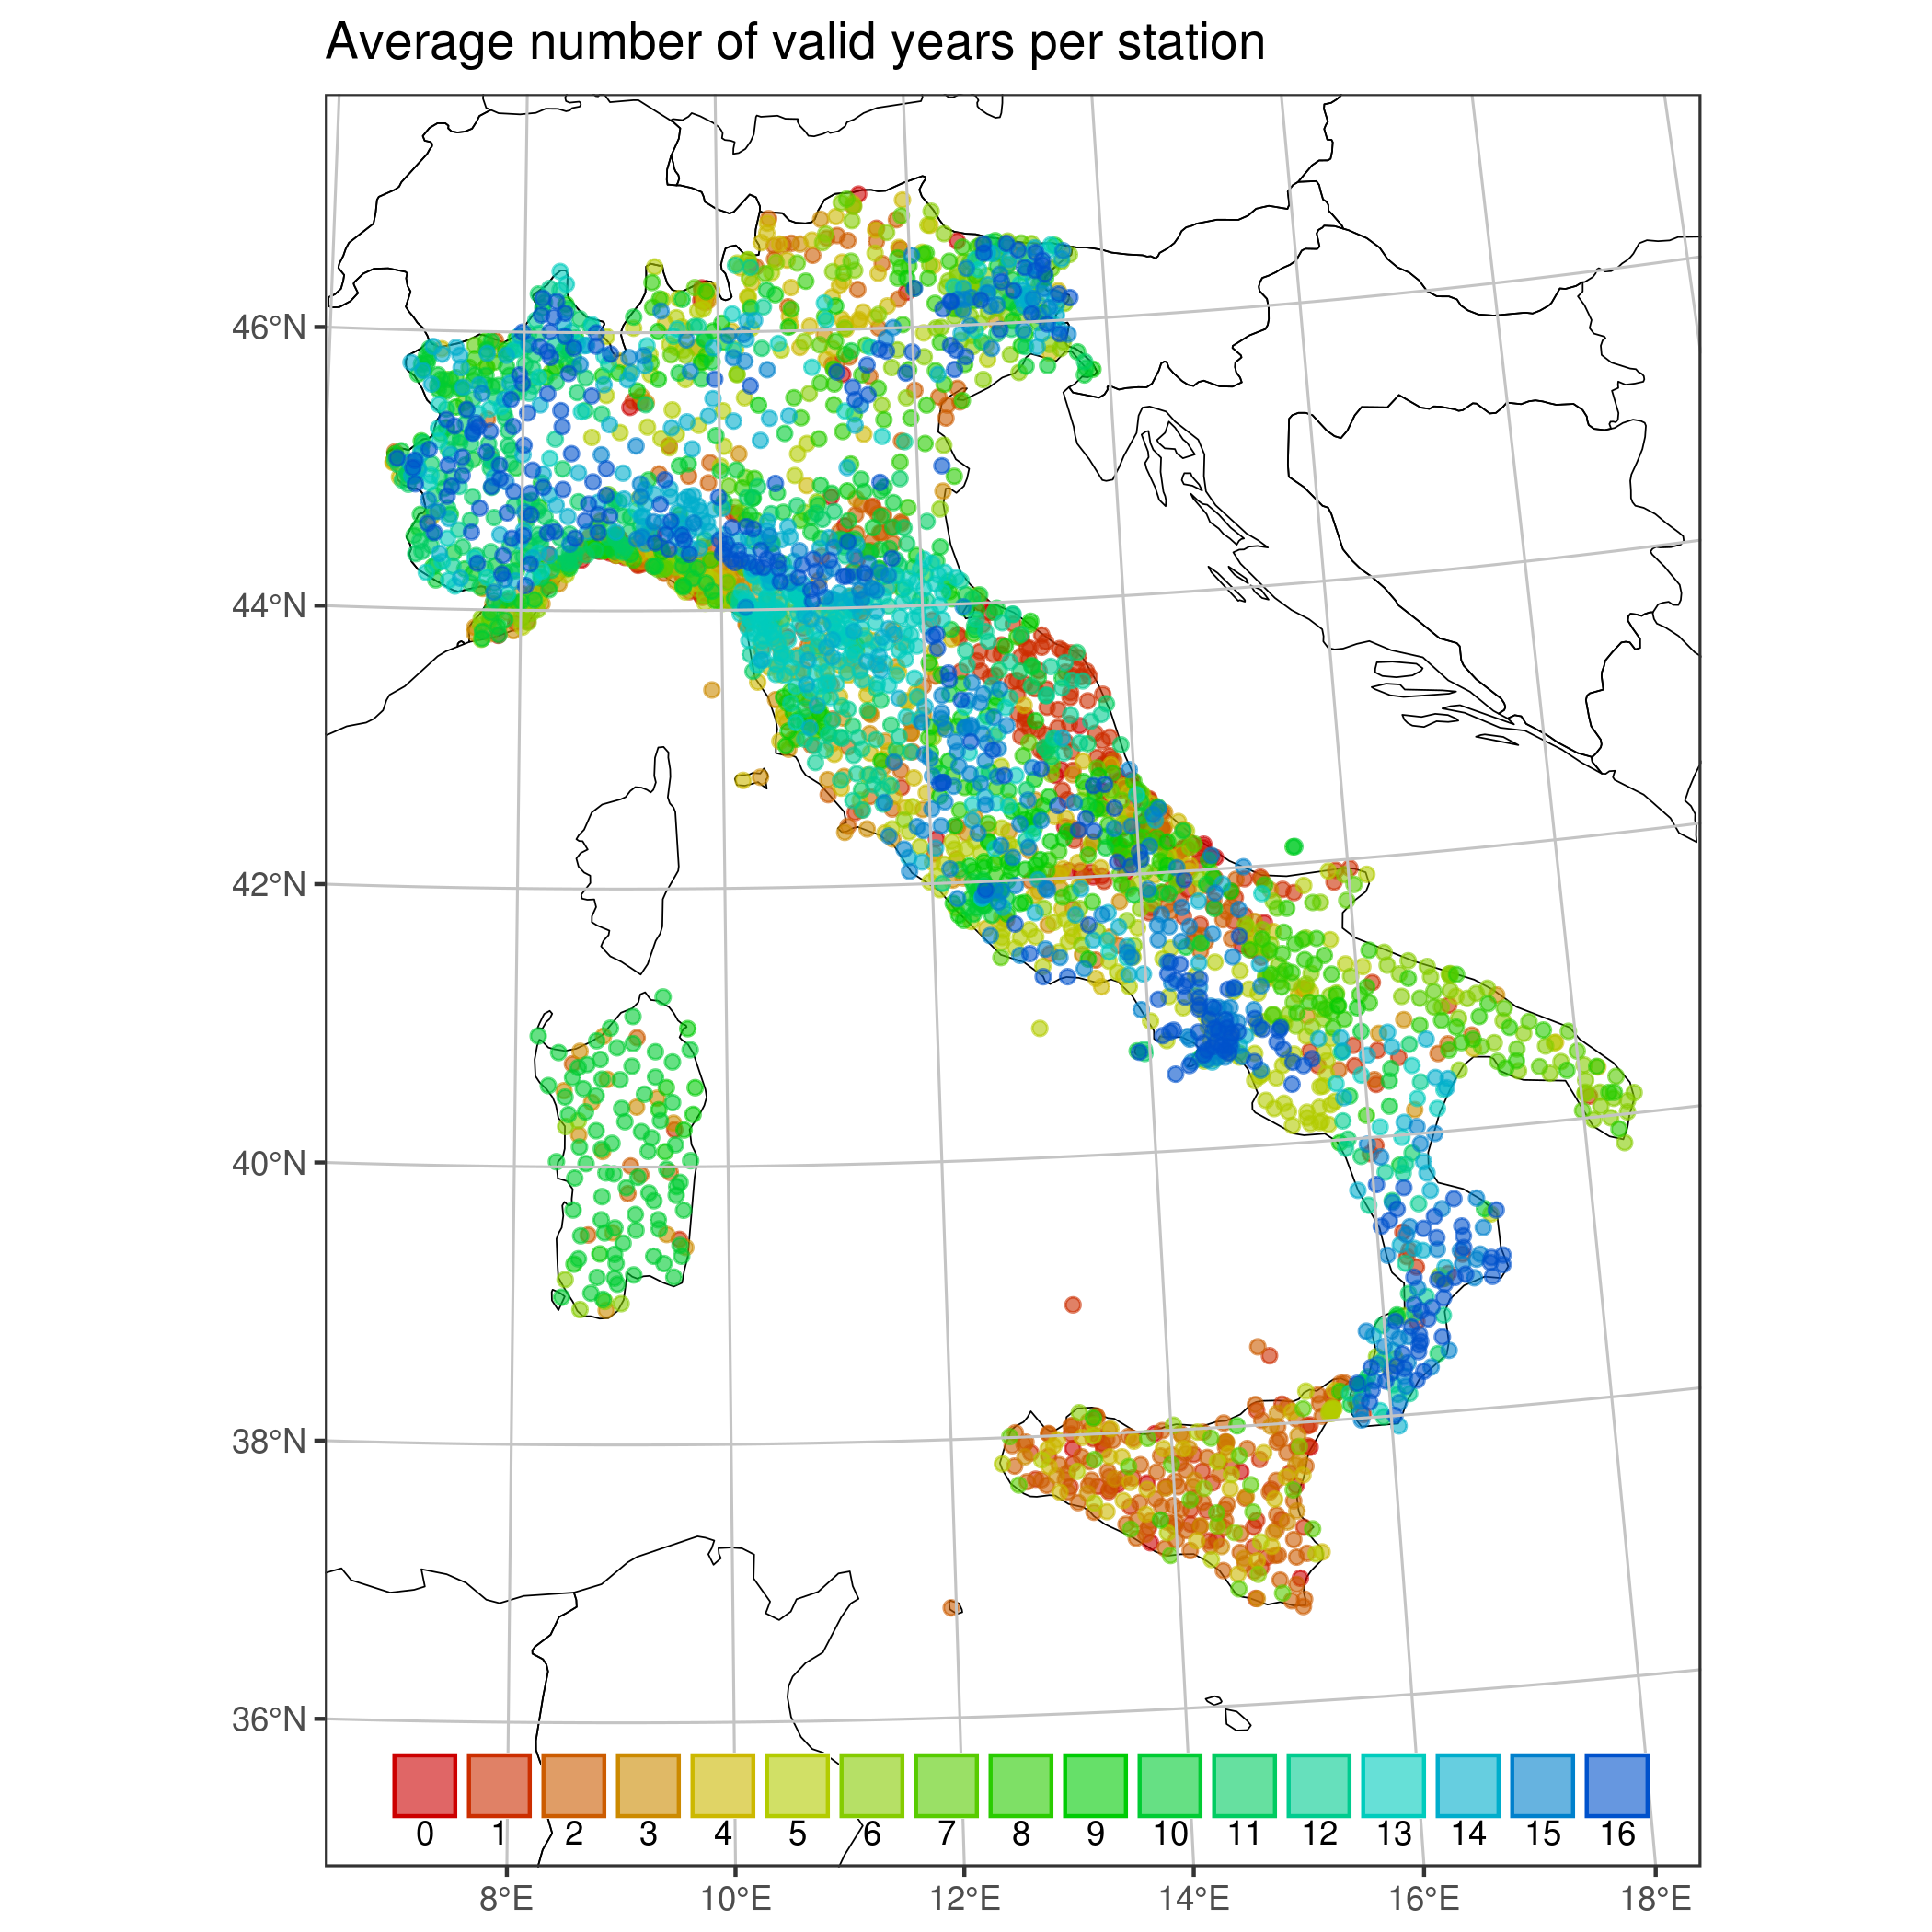
\includegraphics[width=\textwidth]{figures/rain_dst/regional_stats/plot.png}
    \end{subfigure}
    \begin{subfigure}{.475\textwidth}
        \caption{}\label{fig:regional_stats/b}
        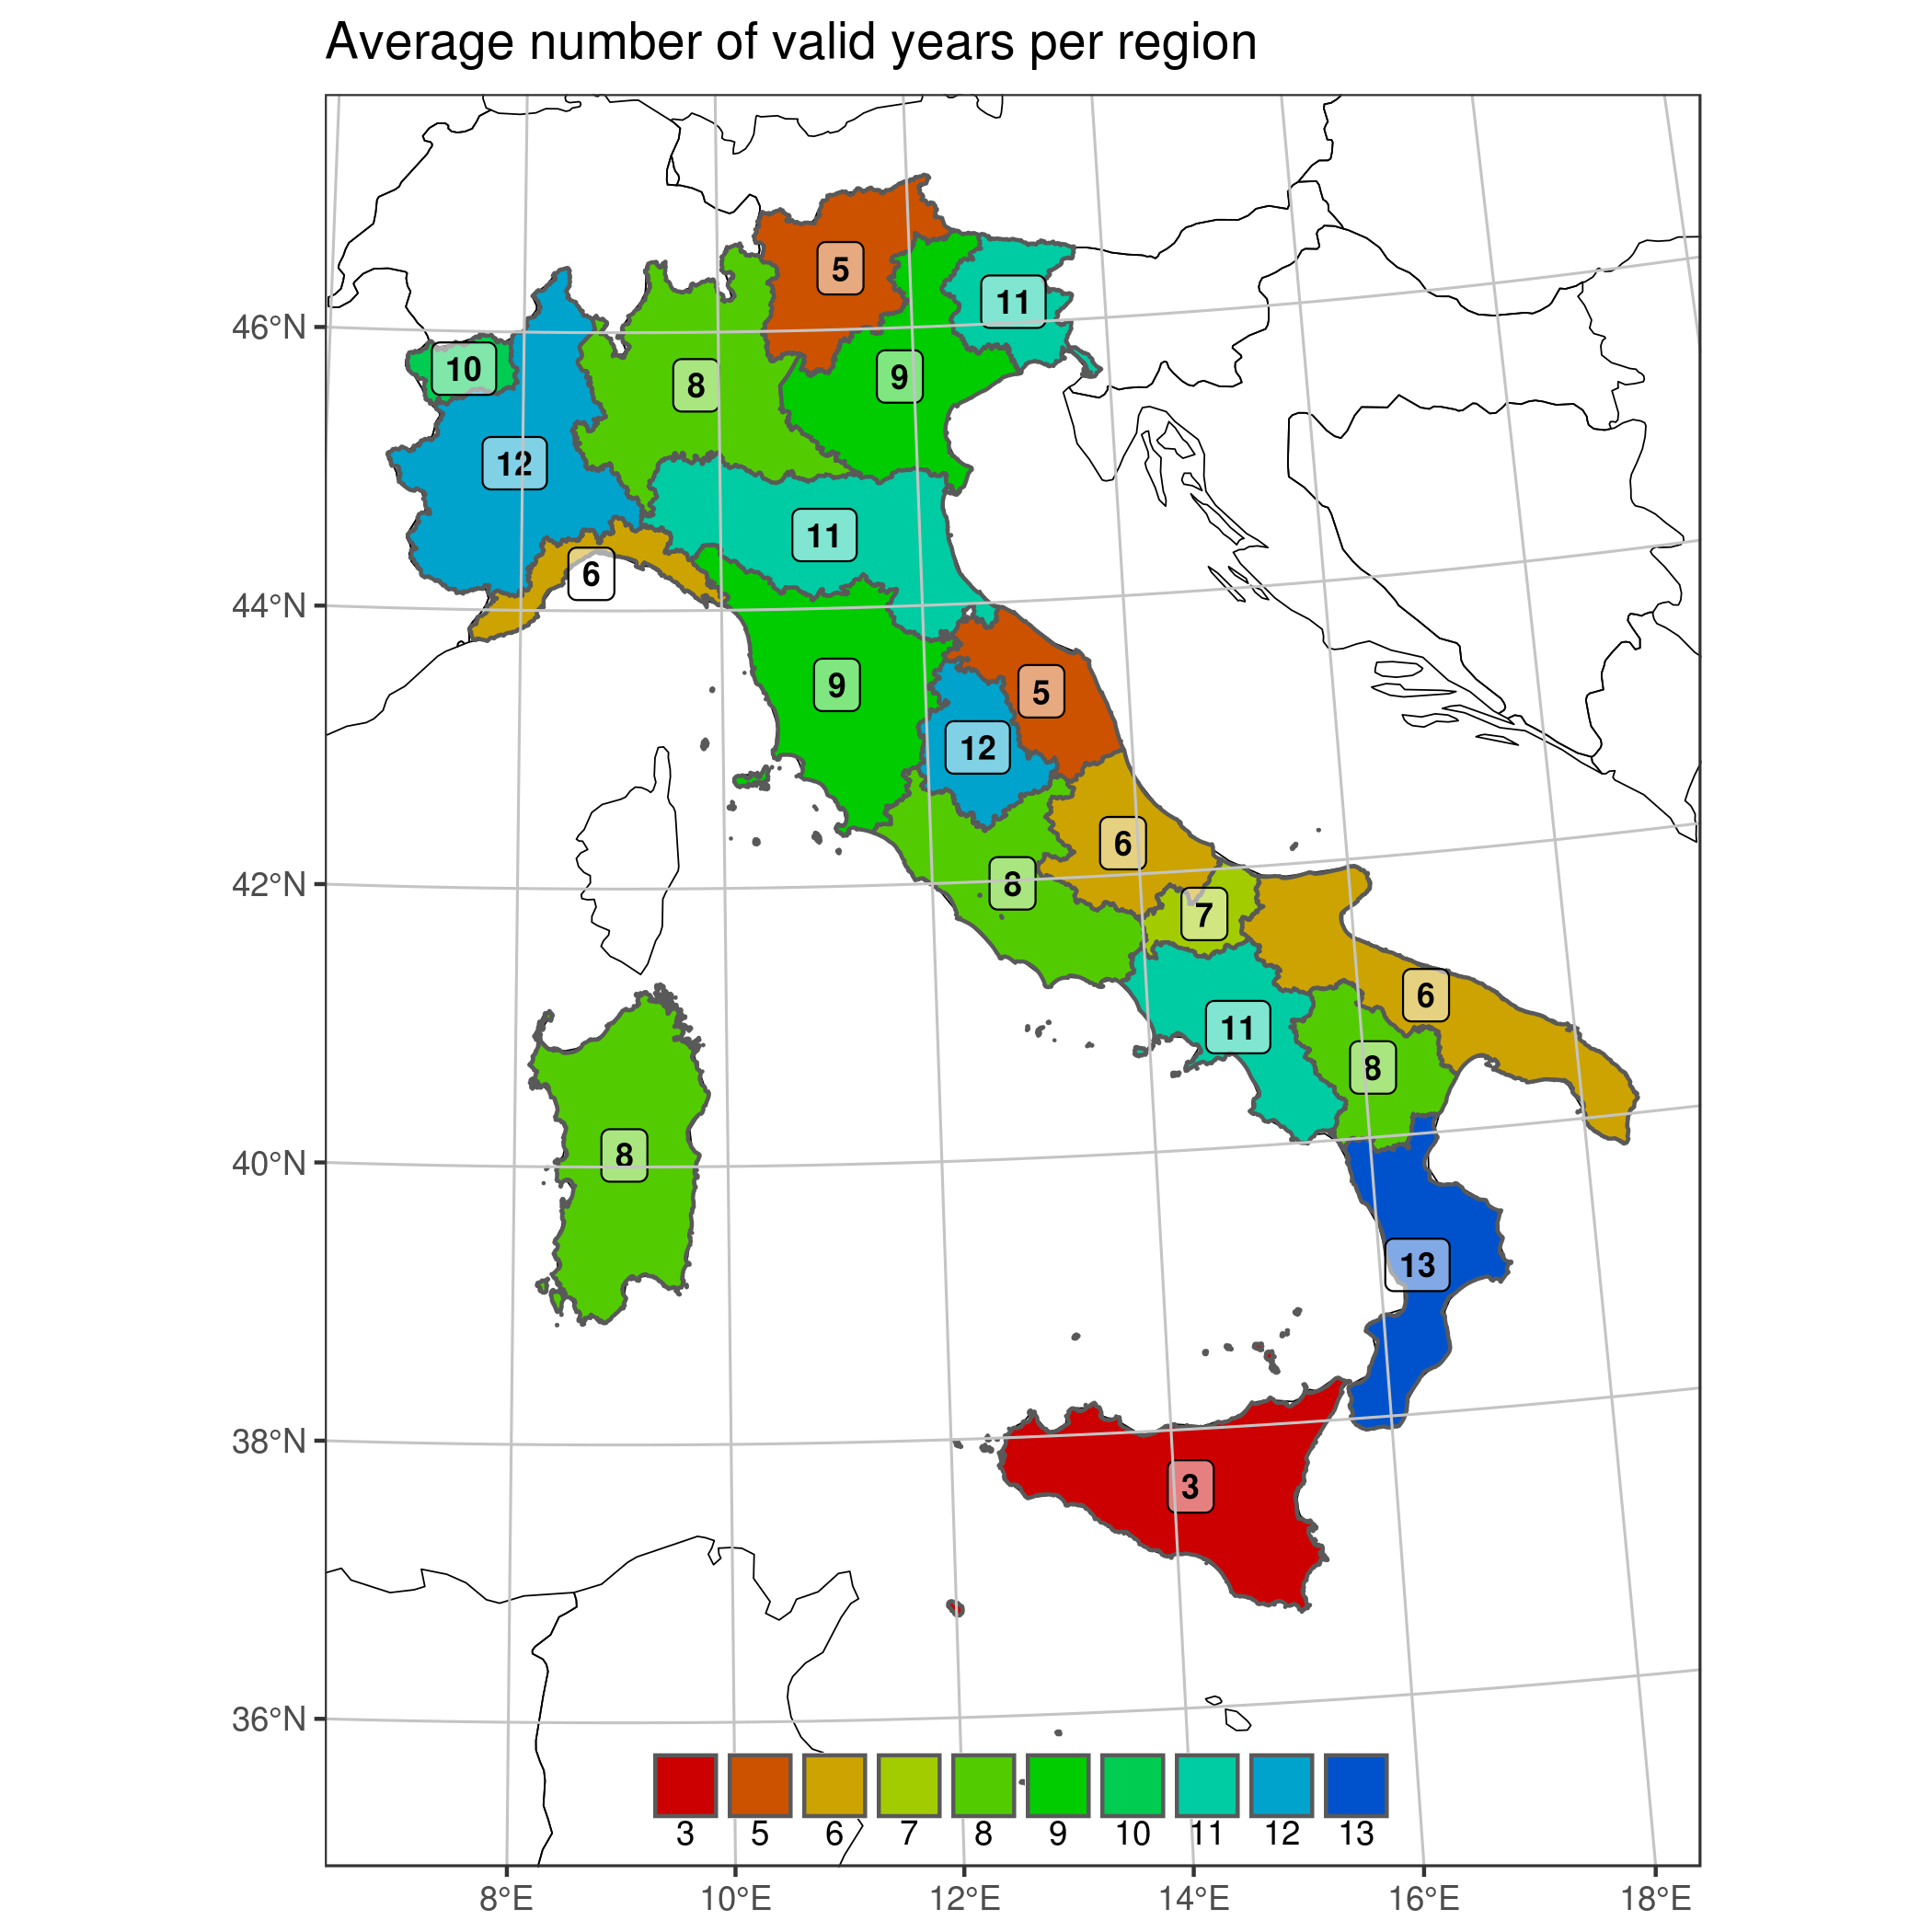
\includegraphics[width=\textwidth]{figures/rain_dst/regional_stats/plot2.png}
    \end{subfigure}\\
    \begin{subfigure}{.475\textwidth}
        \caption{}\label{fig:regional_stats/c}
        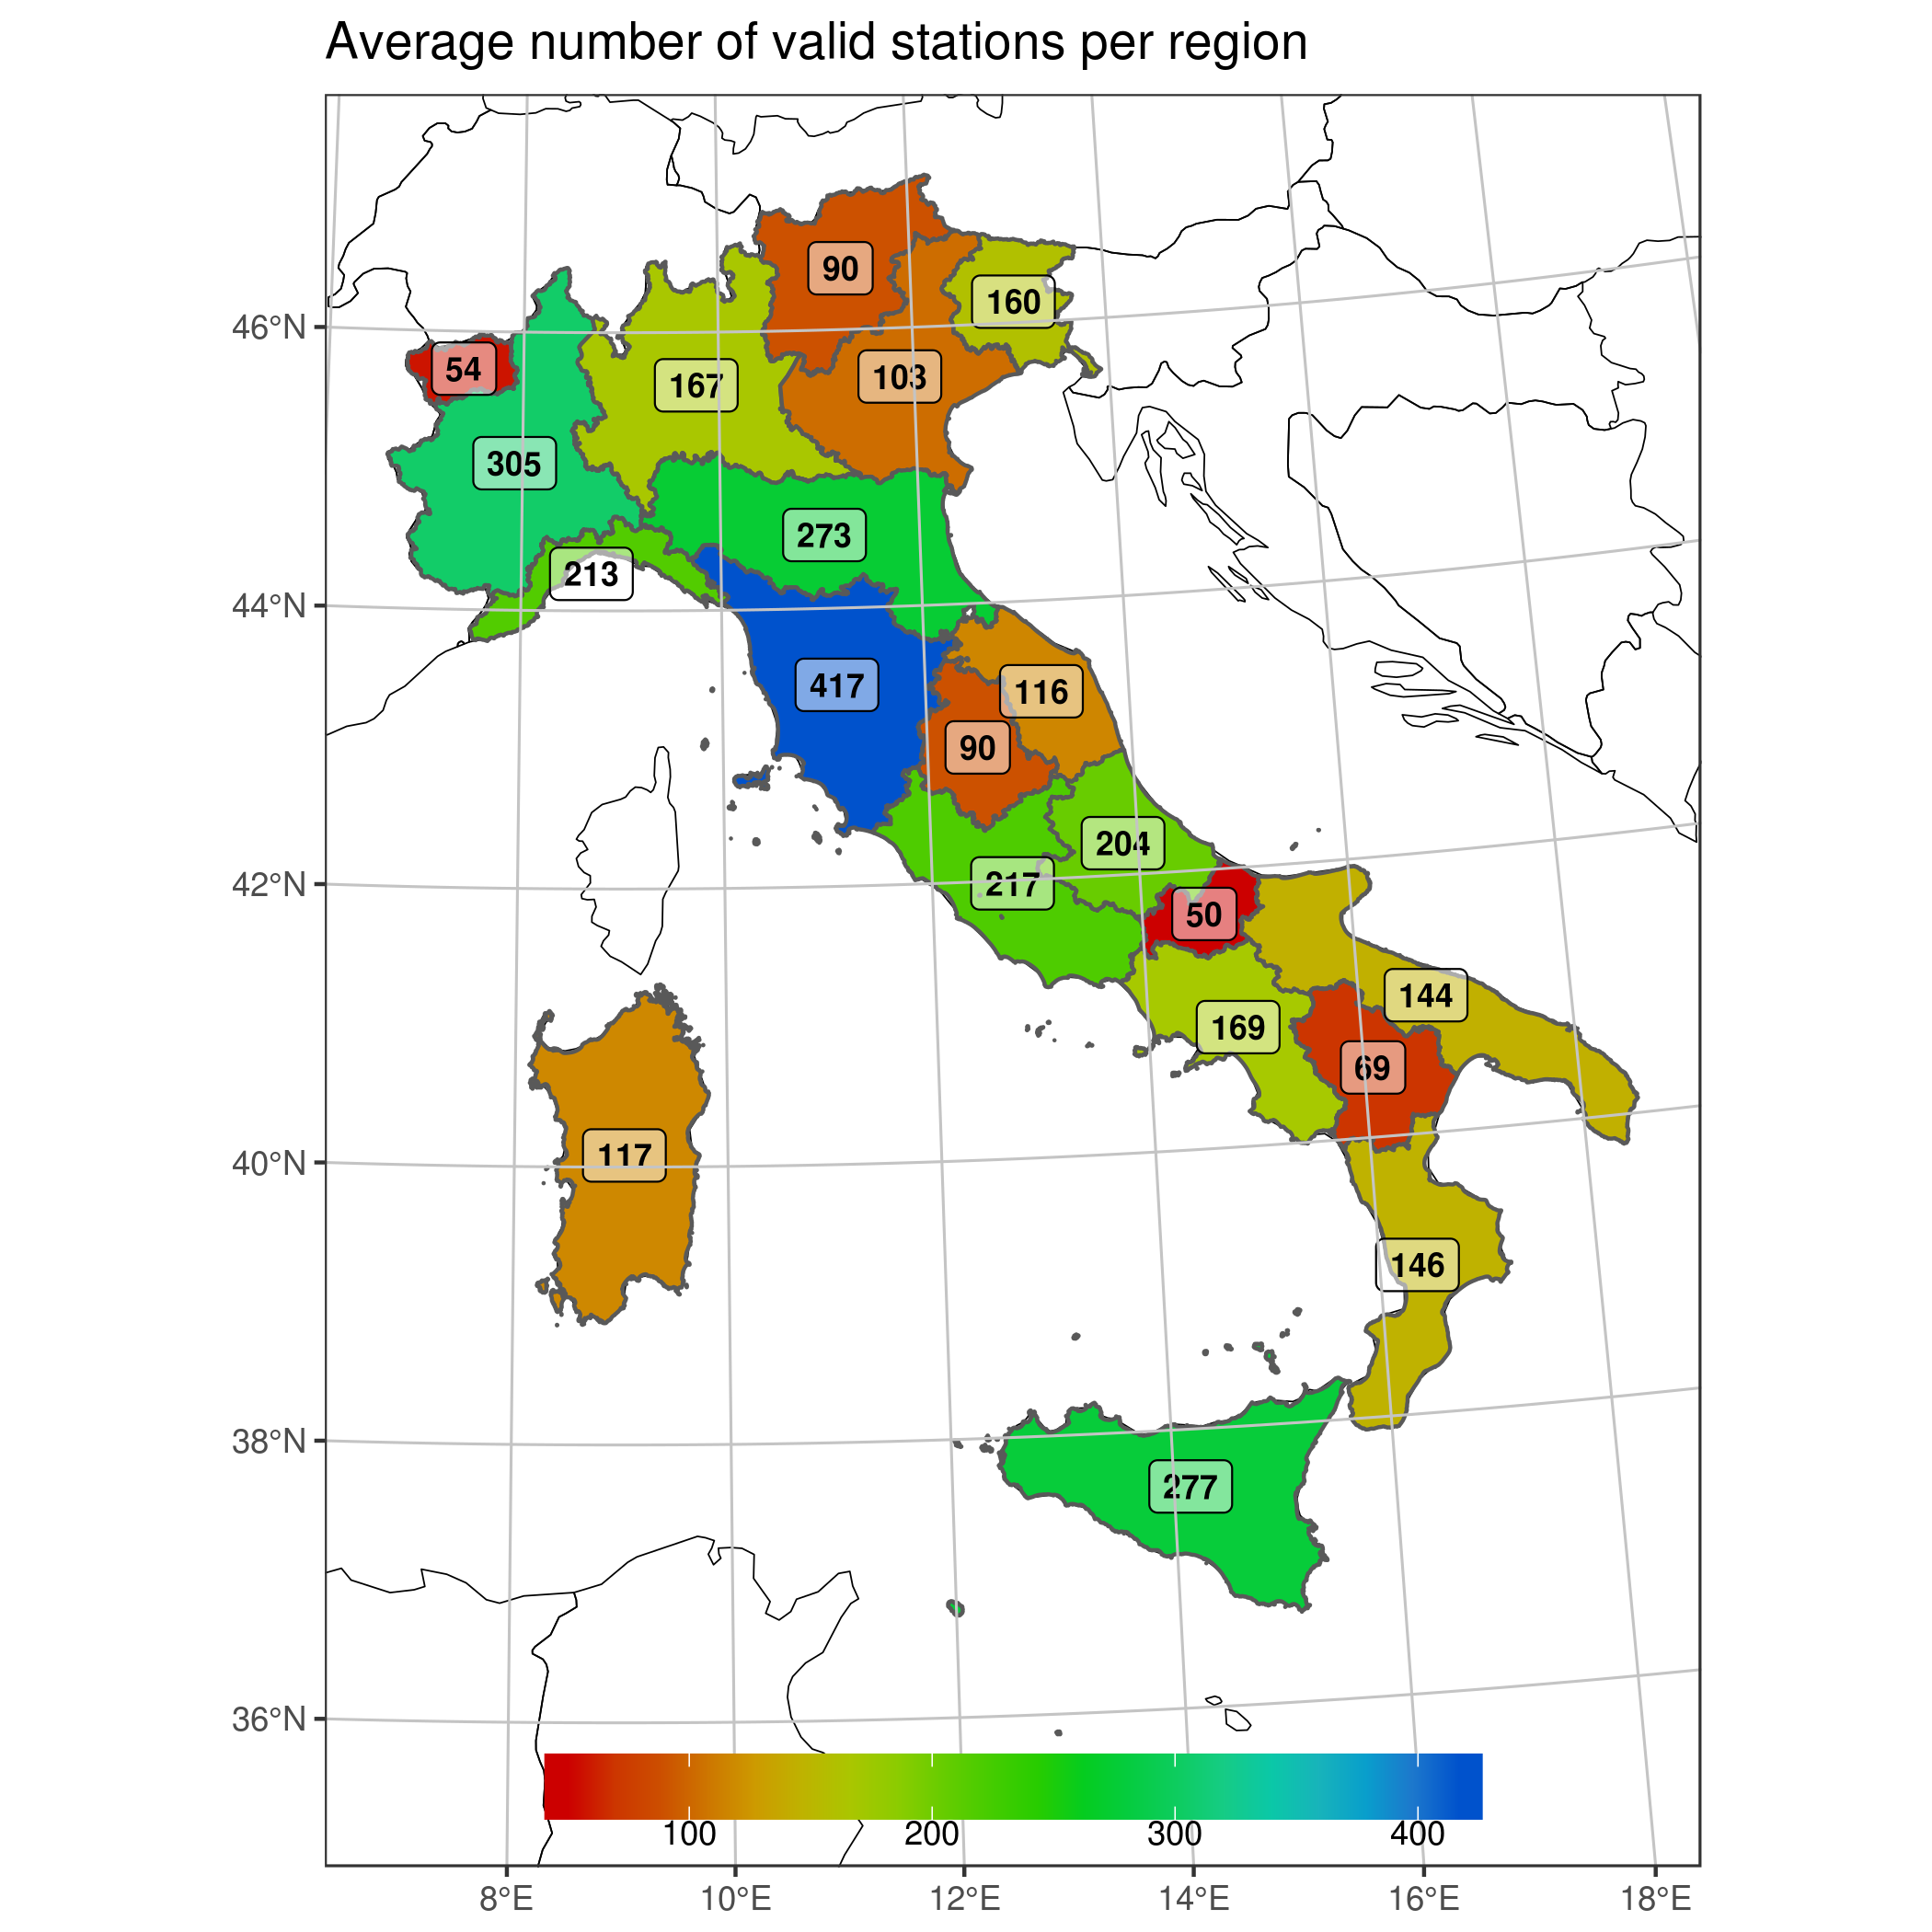
\includegraphics[width=\textwidth]{figures/rain_dst/regional_stats/plot3.png}
    \end{subfigure}
    \begin{subfigure}{.475\textwidth}
        \caption{}\label{fig:regional_stats/d}
        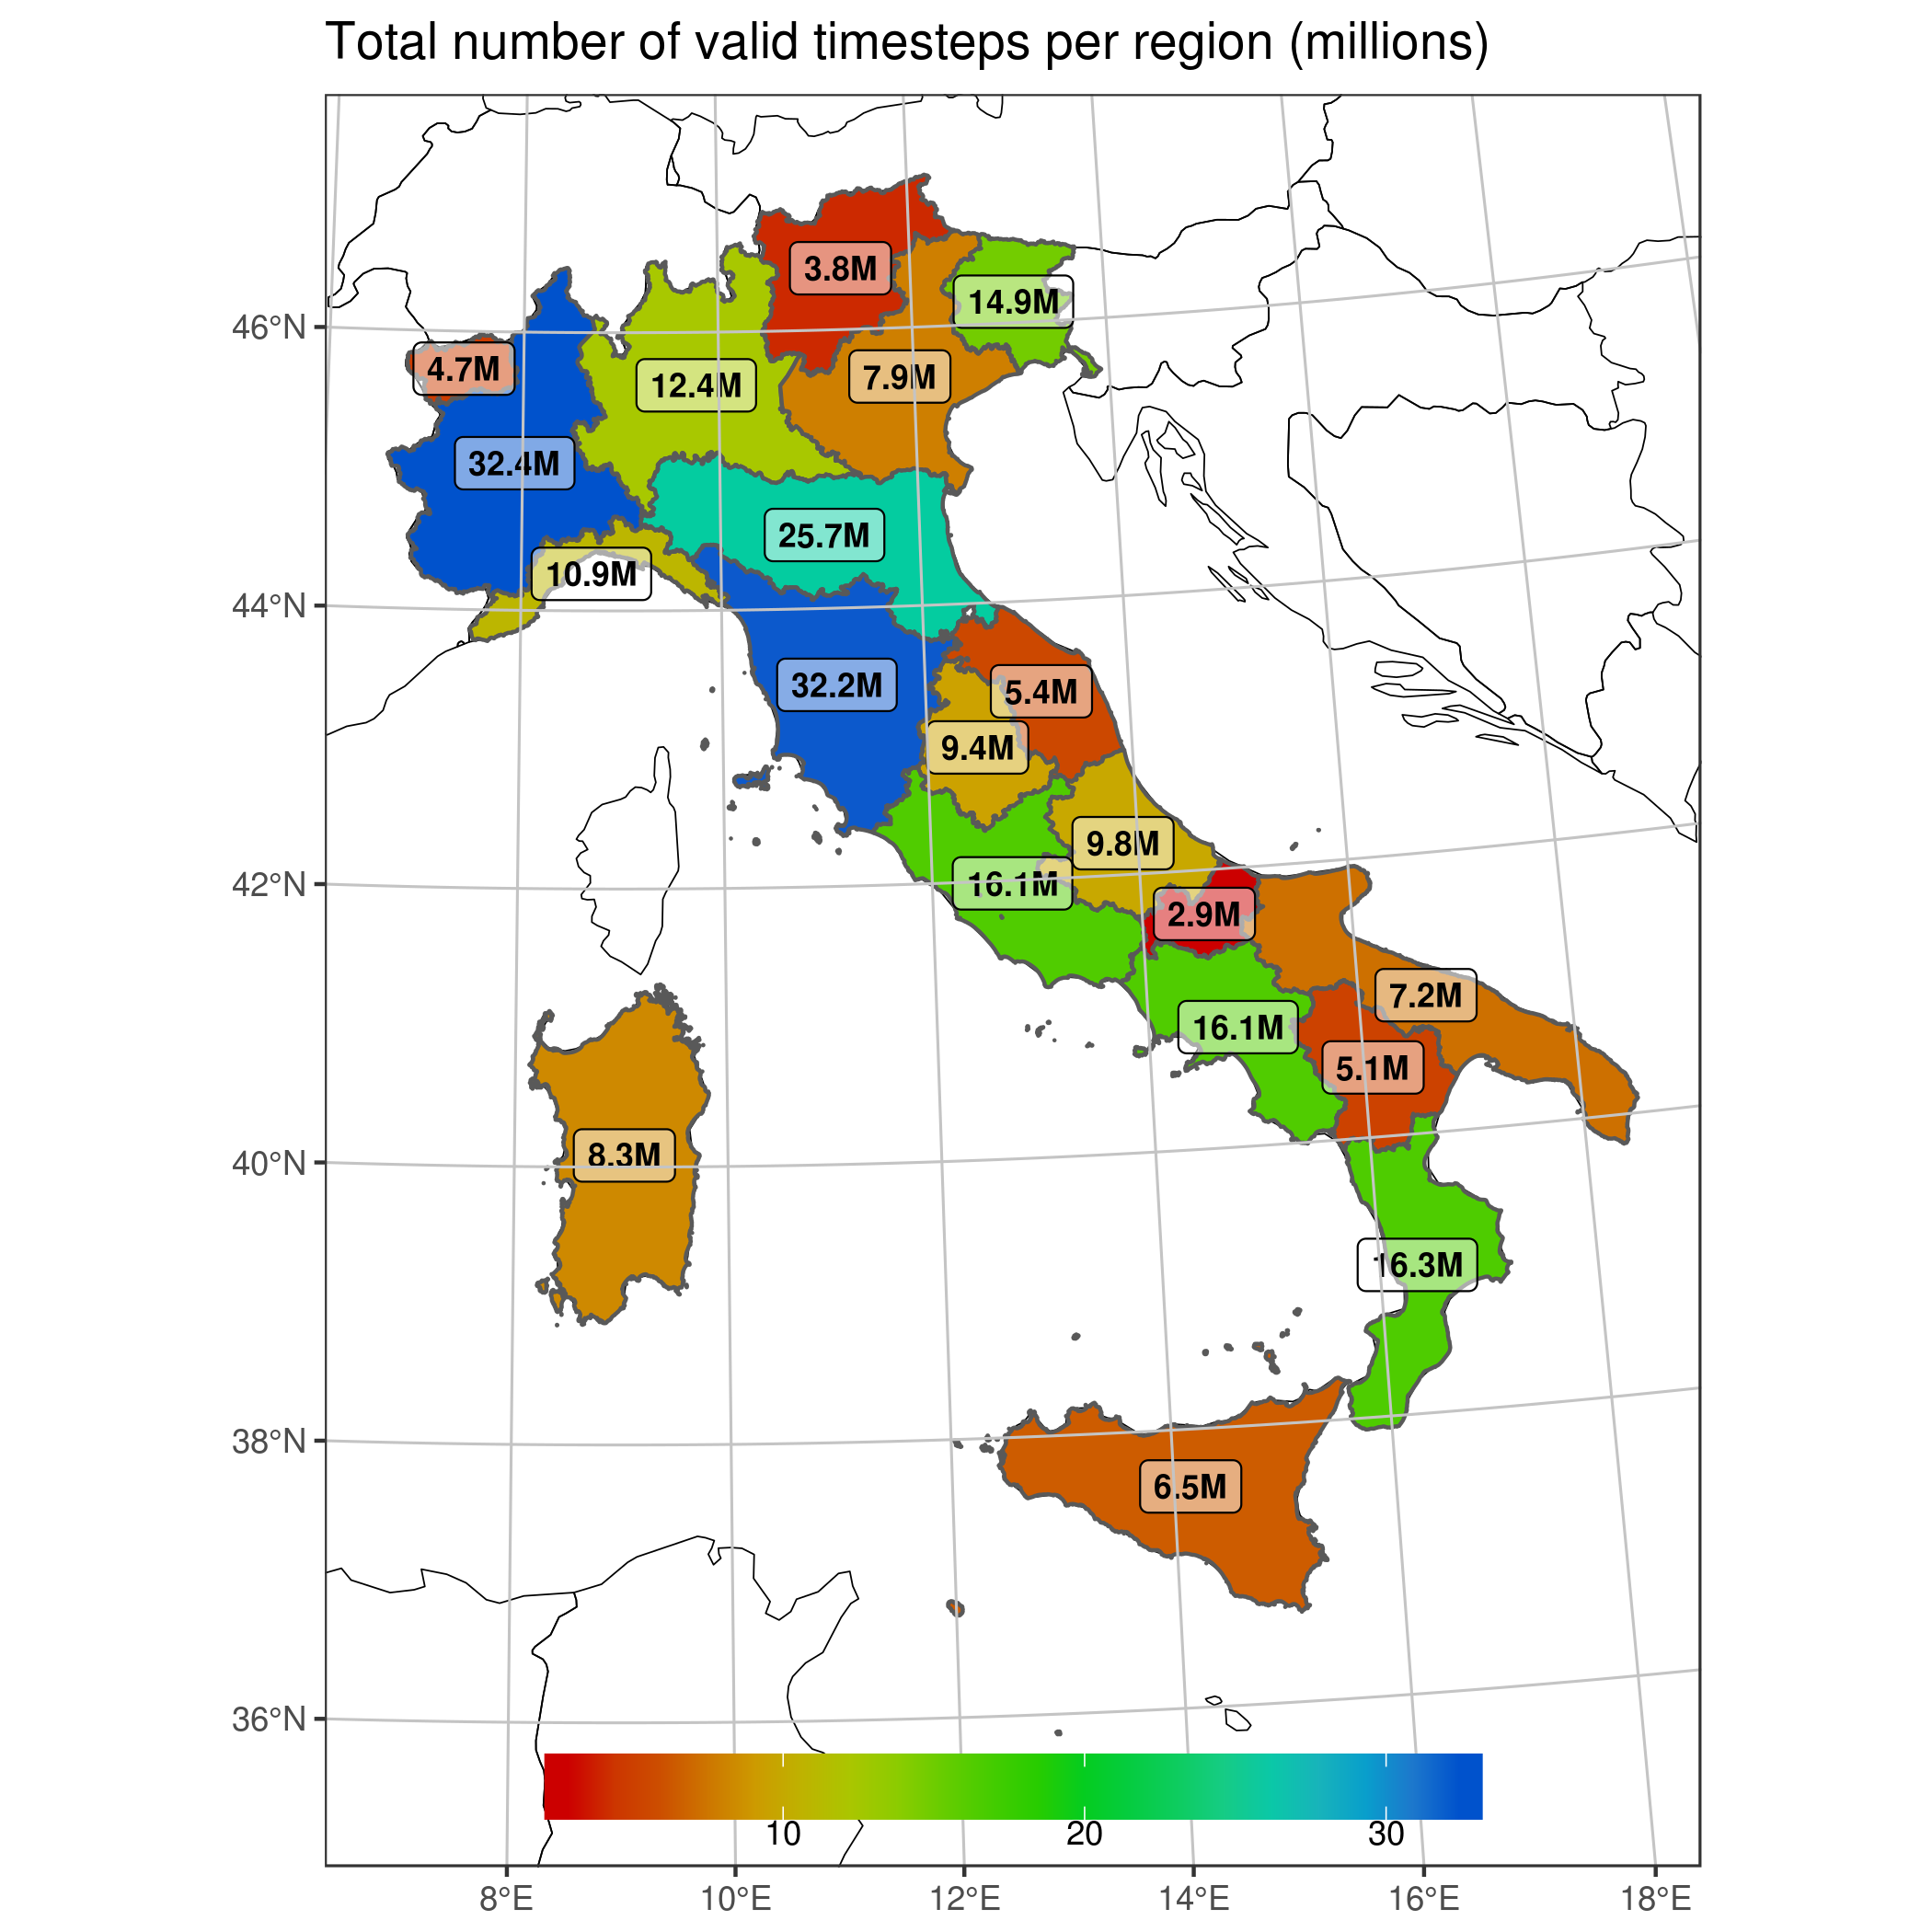
\includegraphics[width=\textwidth]{figures/rain_dst/regional_stats/plot4.png}
    \end{subfigure}\\
    \begin{subfigure}{.475\textwidth}
        \caption{}\label{fig:regional_stats/e}
        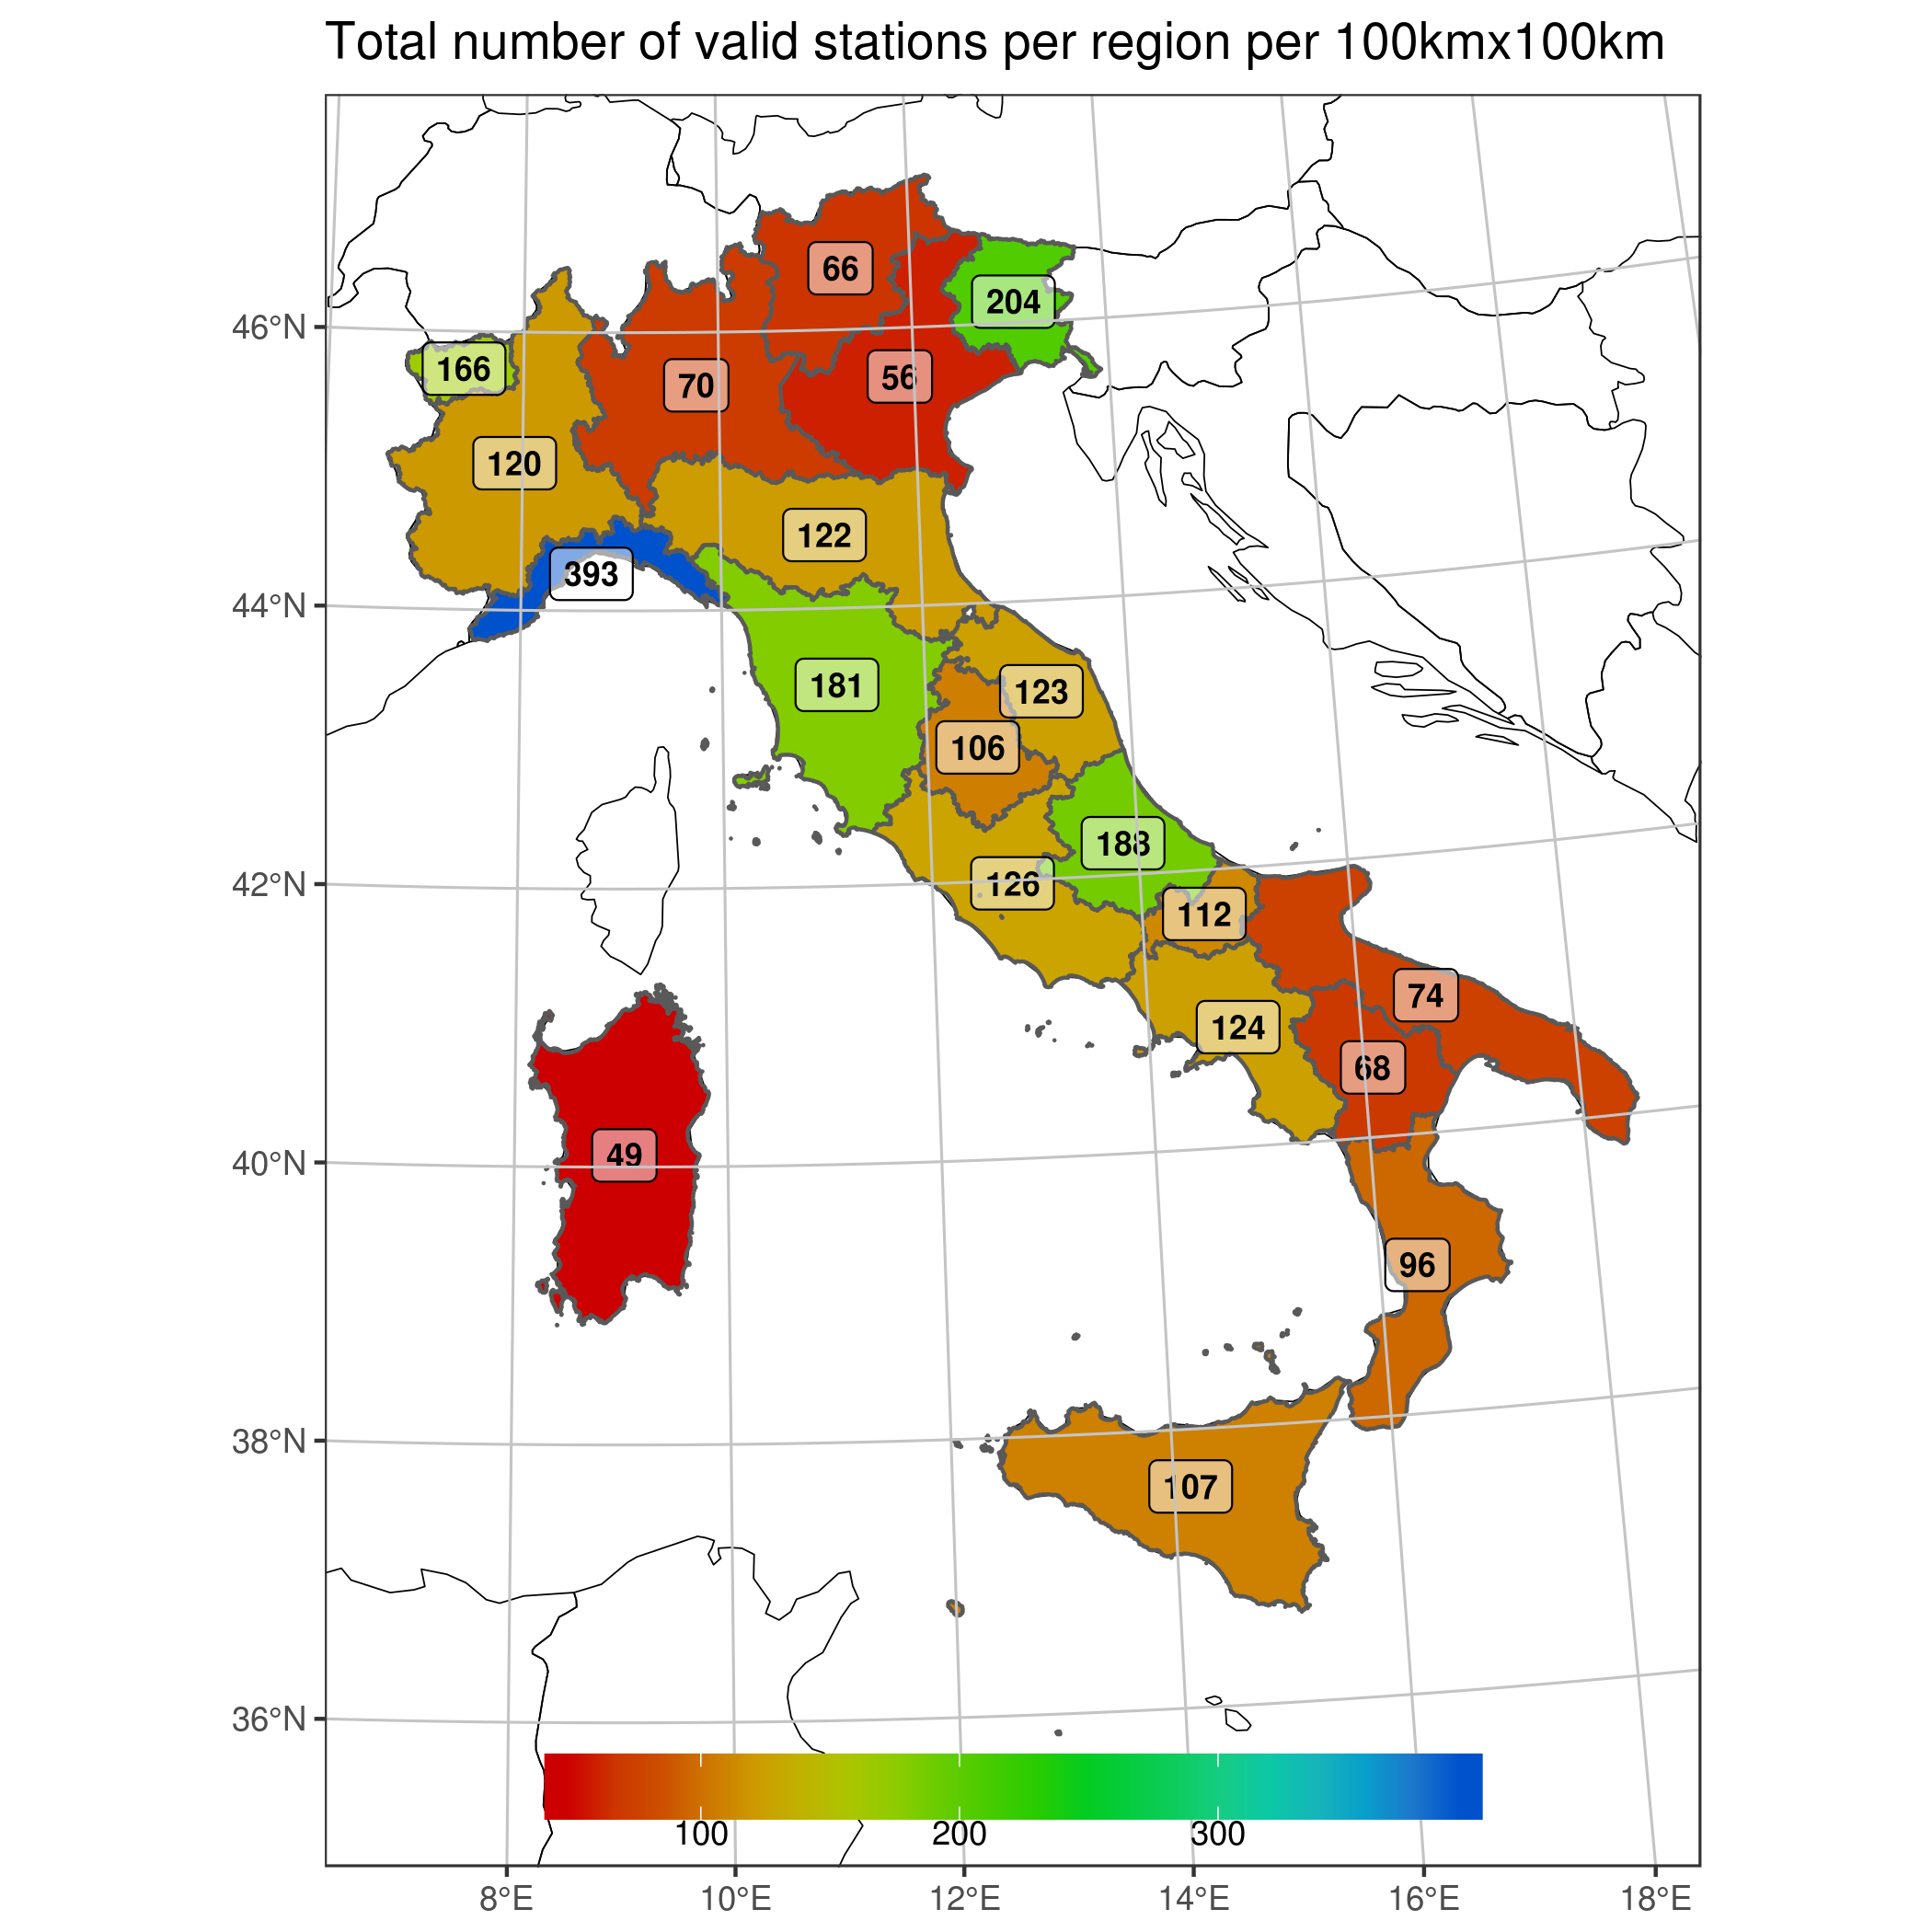
\includegraphics[width=\textwidth]{figures/rain_dst/regional_stats/plot5.png}
    \end{subfigure}
    \begin{subfigure}{.475\textwidth}
        \caption{}\label{fig:regional_stats/f}
        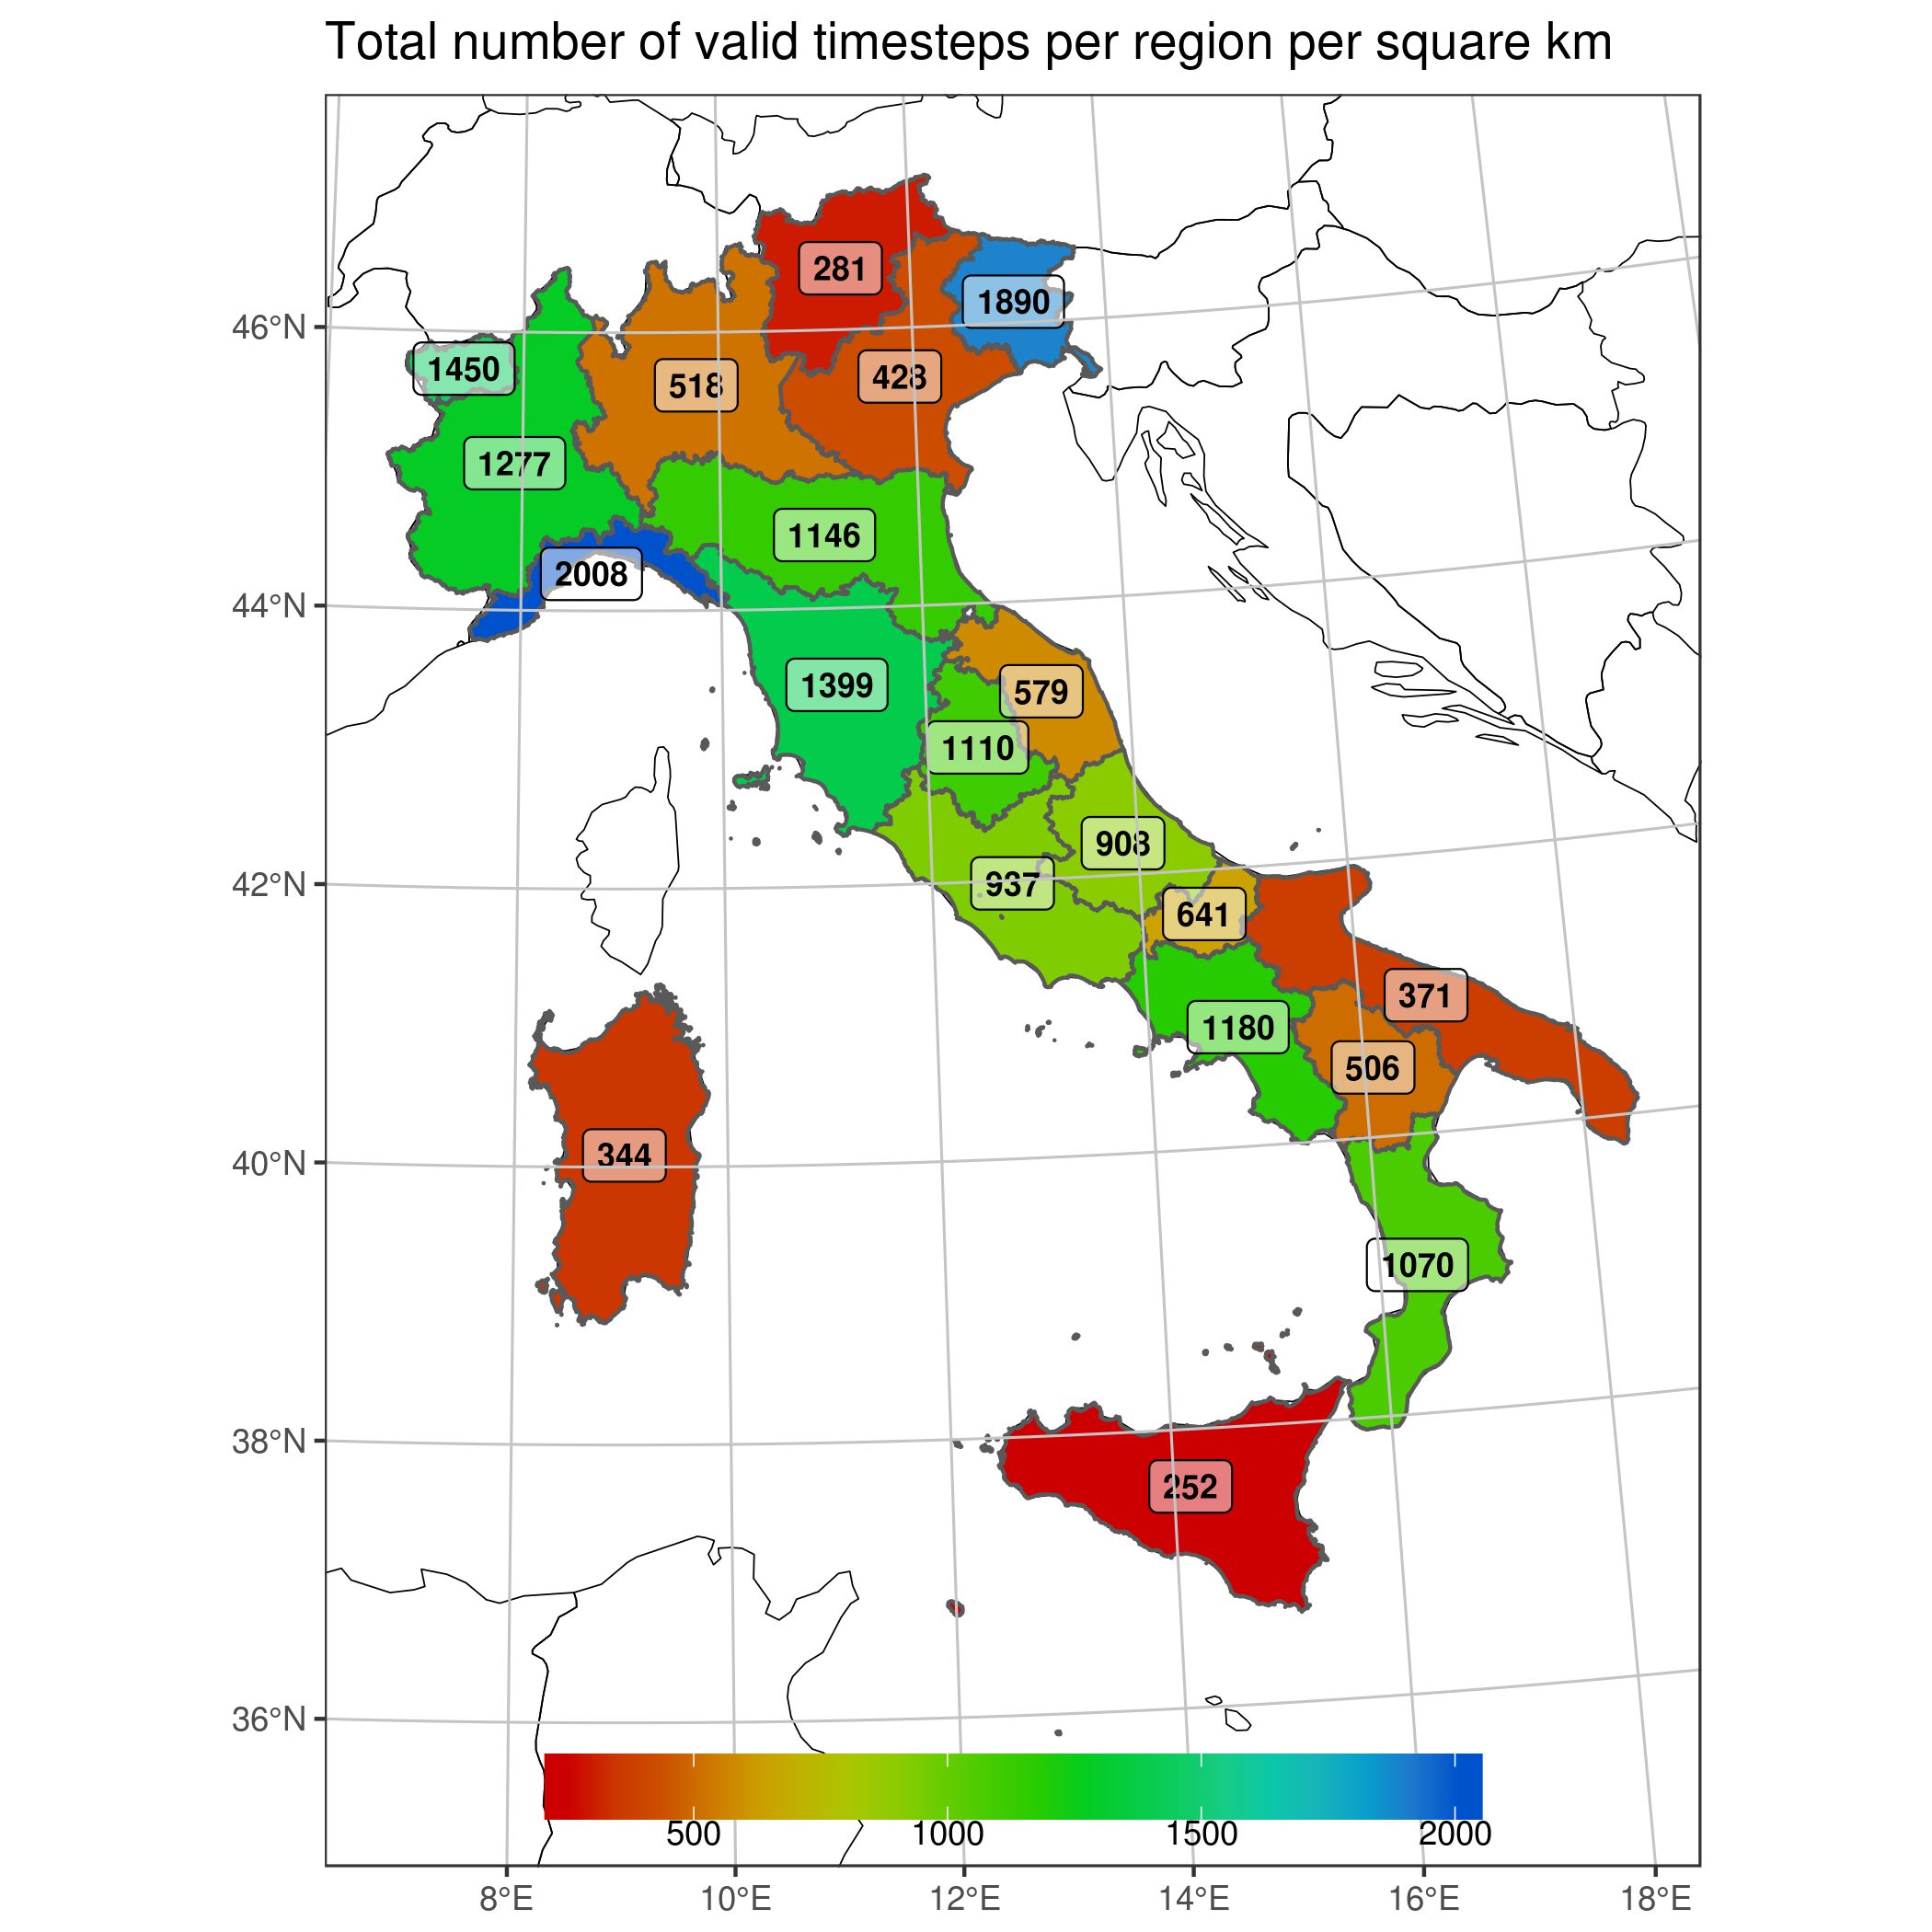
\includegraphics[width=\textwidth]{figures/rain_dst/regional_stats/plot6.png}
    \end{subfigure}
    \decoRule
    \caption[Analysis of station availability for the Italian in-situ hourly precipitation dataset GRIPHO]{Analysis of station availability for the Italian in-situ hourly precipitation dataset GRIPHO; refer to the titles for the contents of each panel} \label{fig:regional_stats}
\end{figure}

As result of this initial analysis a large variability in the data availability is evident. Subsequent analysis (\cref{sec:data_cleaning}) confirms the lack of station coverage for some regions, especially in the early 2000s. Once again, due to the lack of suitable hourly backup data for the whole period and region, these gaps are purposefully left in GRIPHO without any attempt at filling them.

%------------------------------------
%	DATA CHECKING
%------------------------------------
\section{Data checking, flagging and cleaning} \label{sec:data_cleaning}
Due to the fragmented nature of the data, which comes from a plethora of different regional agencies, the original data provider could not guarantee that any quality control procedure or checks were performed on the station data.
As a result, understanding which eventual problems affect the input data represents the first priority in order to reduce the bias in the final product.\\ %***TODO*** add here a brief literature review on precipitation data cleaning
Several procedures are carried out in order to identify and remove errors and inconsistencies, such as:
\begin{itemize}
    \item analysing spatial and temporal distribution of the stations (\cref{fig:stat_distr_height,fig:stat_avail_ts}), also separated by region (\cref{fig:regional_stats});
    \item producing precipitation maps for each timestep and assembling into videos;
    \item manually analysing single station timeseries;
    \item automatic flagging of suspicious events in single station timeseries;
    \item automatic removal of extremely suspicious events;
    \item manual checking of monthly precipitation maps and statistics over the whole time period;
\end{itemize}
Due to the complexity of such procedure, no correction is attempted for those values that resulted to be erroneous or suspicious; additionally, no undercatch correction (see \cref{sec:gauge_undercatch}) is applied due to the lack of the sufficient station metadata.

\subsection{Station-by-station timeseries analysis and flagging}
A manual temporal analysis was carried out independently for all 3712 stations in the original dataset. During this process several inconsistencies were discovered, in particular:
\begin{itemize}
    \item the vast majority of data points are stored in round hours timesteps (timestamps ending in `:00' minutes), with only a handful values (less than 0.1\%) stored in between. This indicates that most of the data is actually hourly, and not sub-hourly.
    \item Some stations (see e.g.\ \cref{fig:ts_rain/a}) seem to suffer from issues with stuck sensors, causing constant values to be reported for very long periods of time. This occurs most often with the \SI{0}{\milli\metre\per\hour} value, but some instances of constant values differing from zero (most often values close to zero) are present.
    \item A sizeable amount of extremely high outliers (see e.g.\ \cref{fig:ts_rain/b}) was detected. Sometimes this affects only a single station in a given area, indicating a fluke or error in the instrumentation; other times several neighbouring stations appear to show the same behaviour, indicating an issue in the data collection and processing.
\end{itemize}

\begin{figure}
    \centering
    % source of this data if you want to remake it:
    % /home/clima-archive/afantini/flood/museodat2nc/dewrain_2000-2016/plots/
    \begin{subfigure}{\textwidth}
        \caption{}\label{fig:ts_rain/a}
        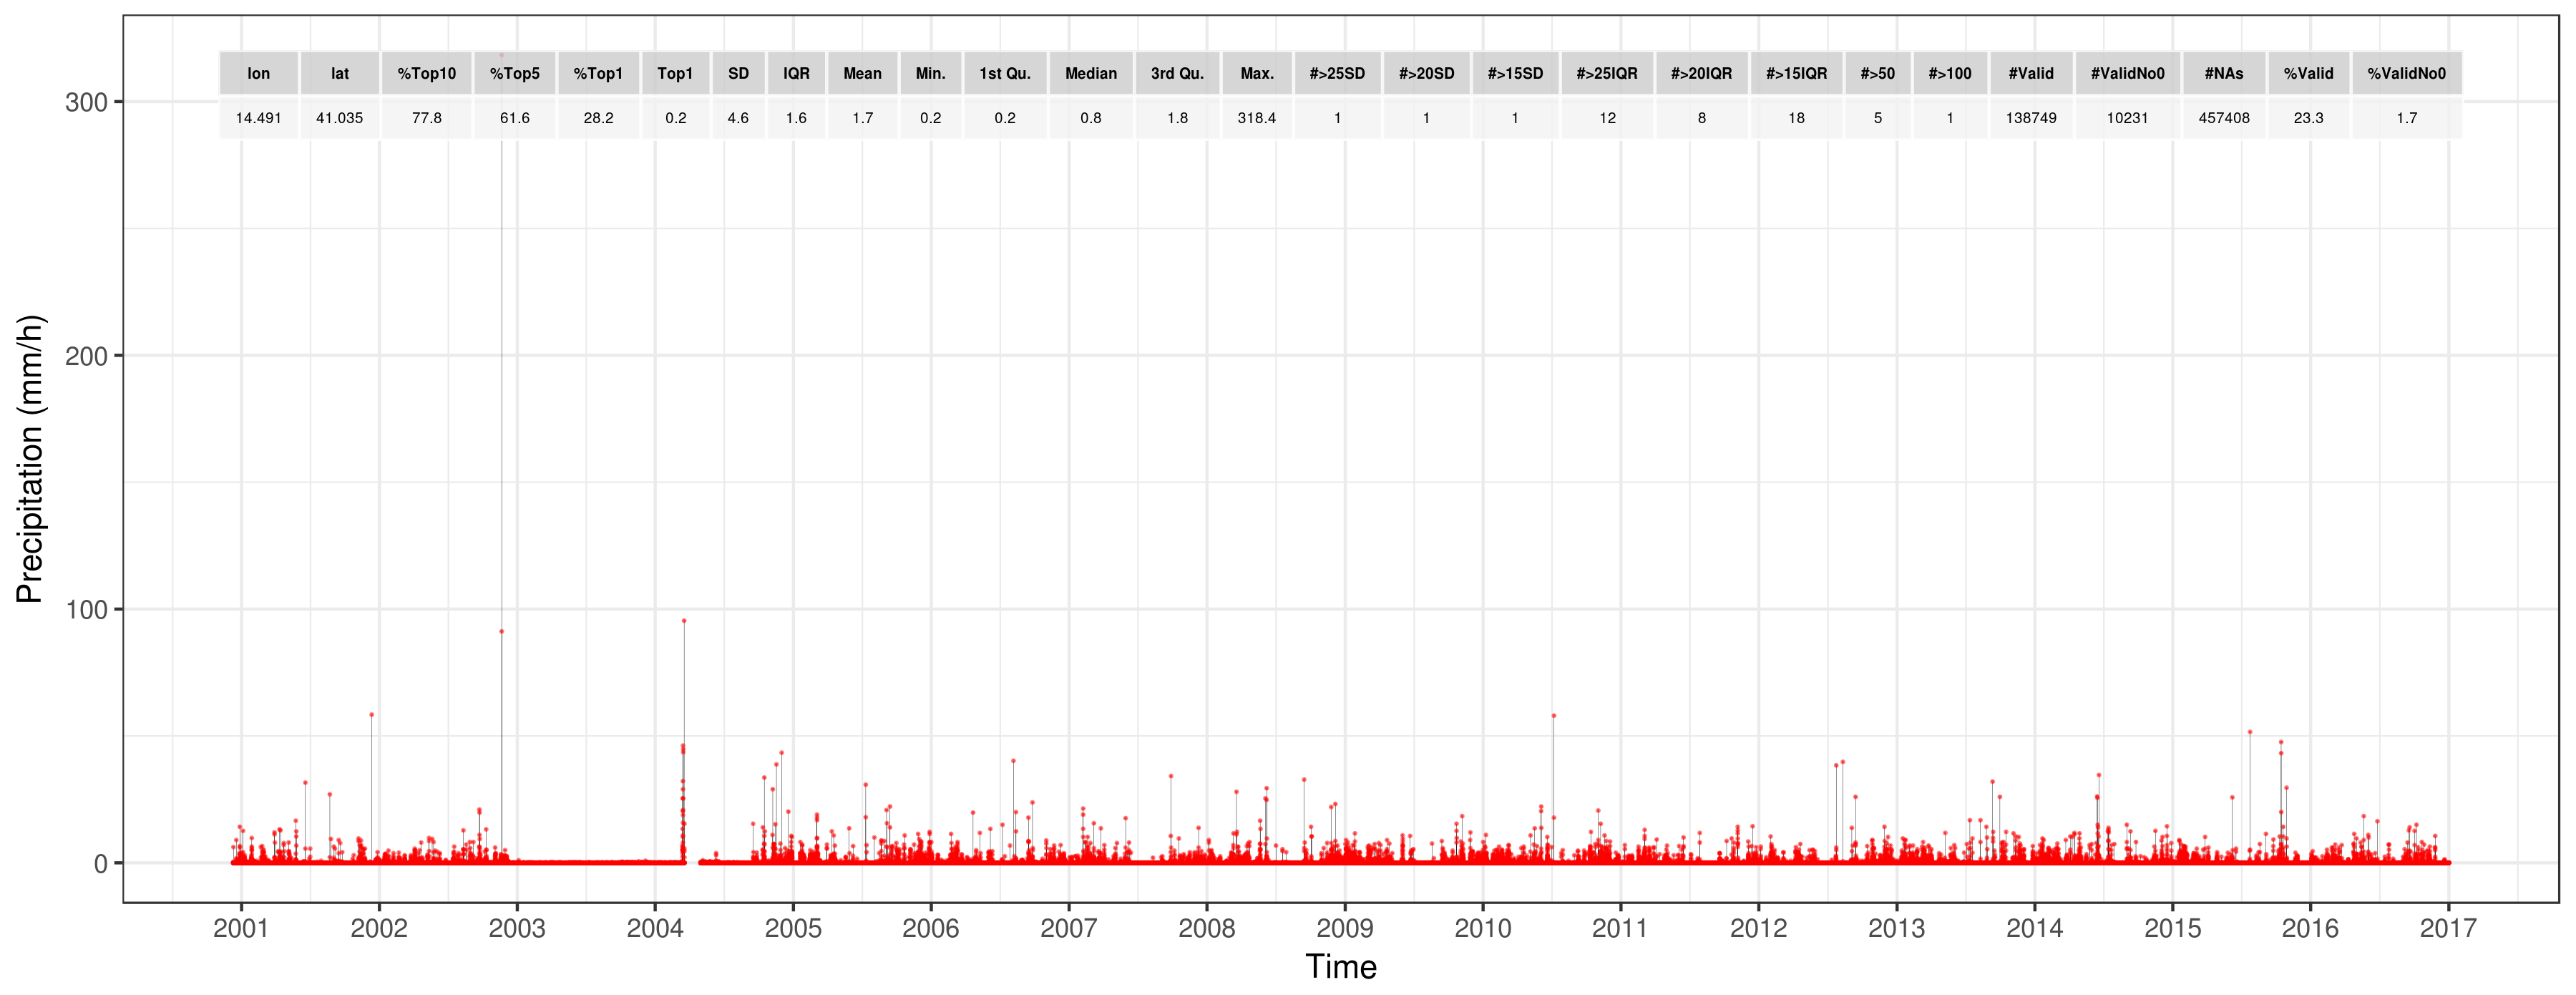
\includegraphics[width=\textwidth]{figures/rain_dst/63_ts.png}
    \end{subfigure}\\
    \begin{subfigure}{\textwidth}
        \caption{}\label{fig:ts_rain/b}
        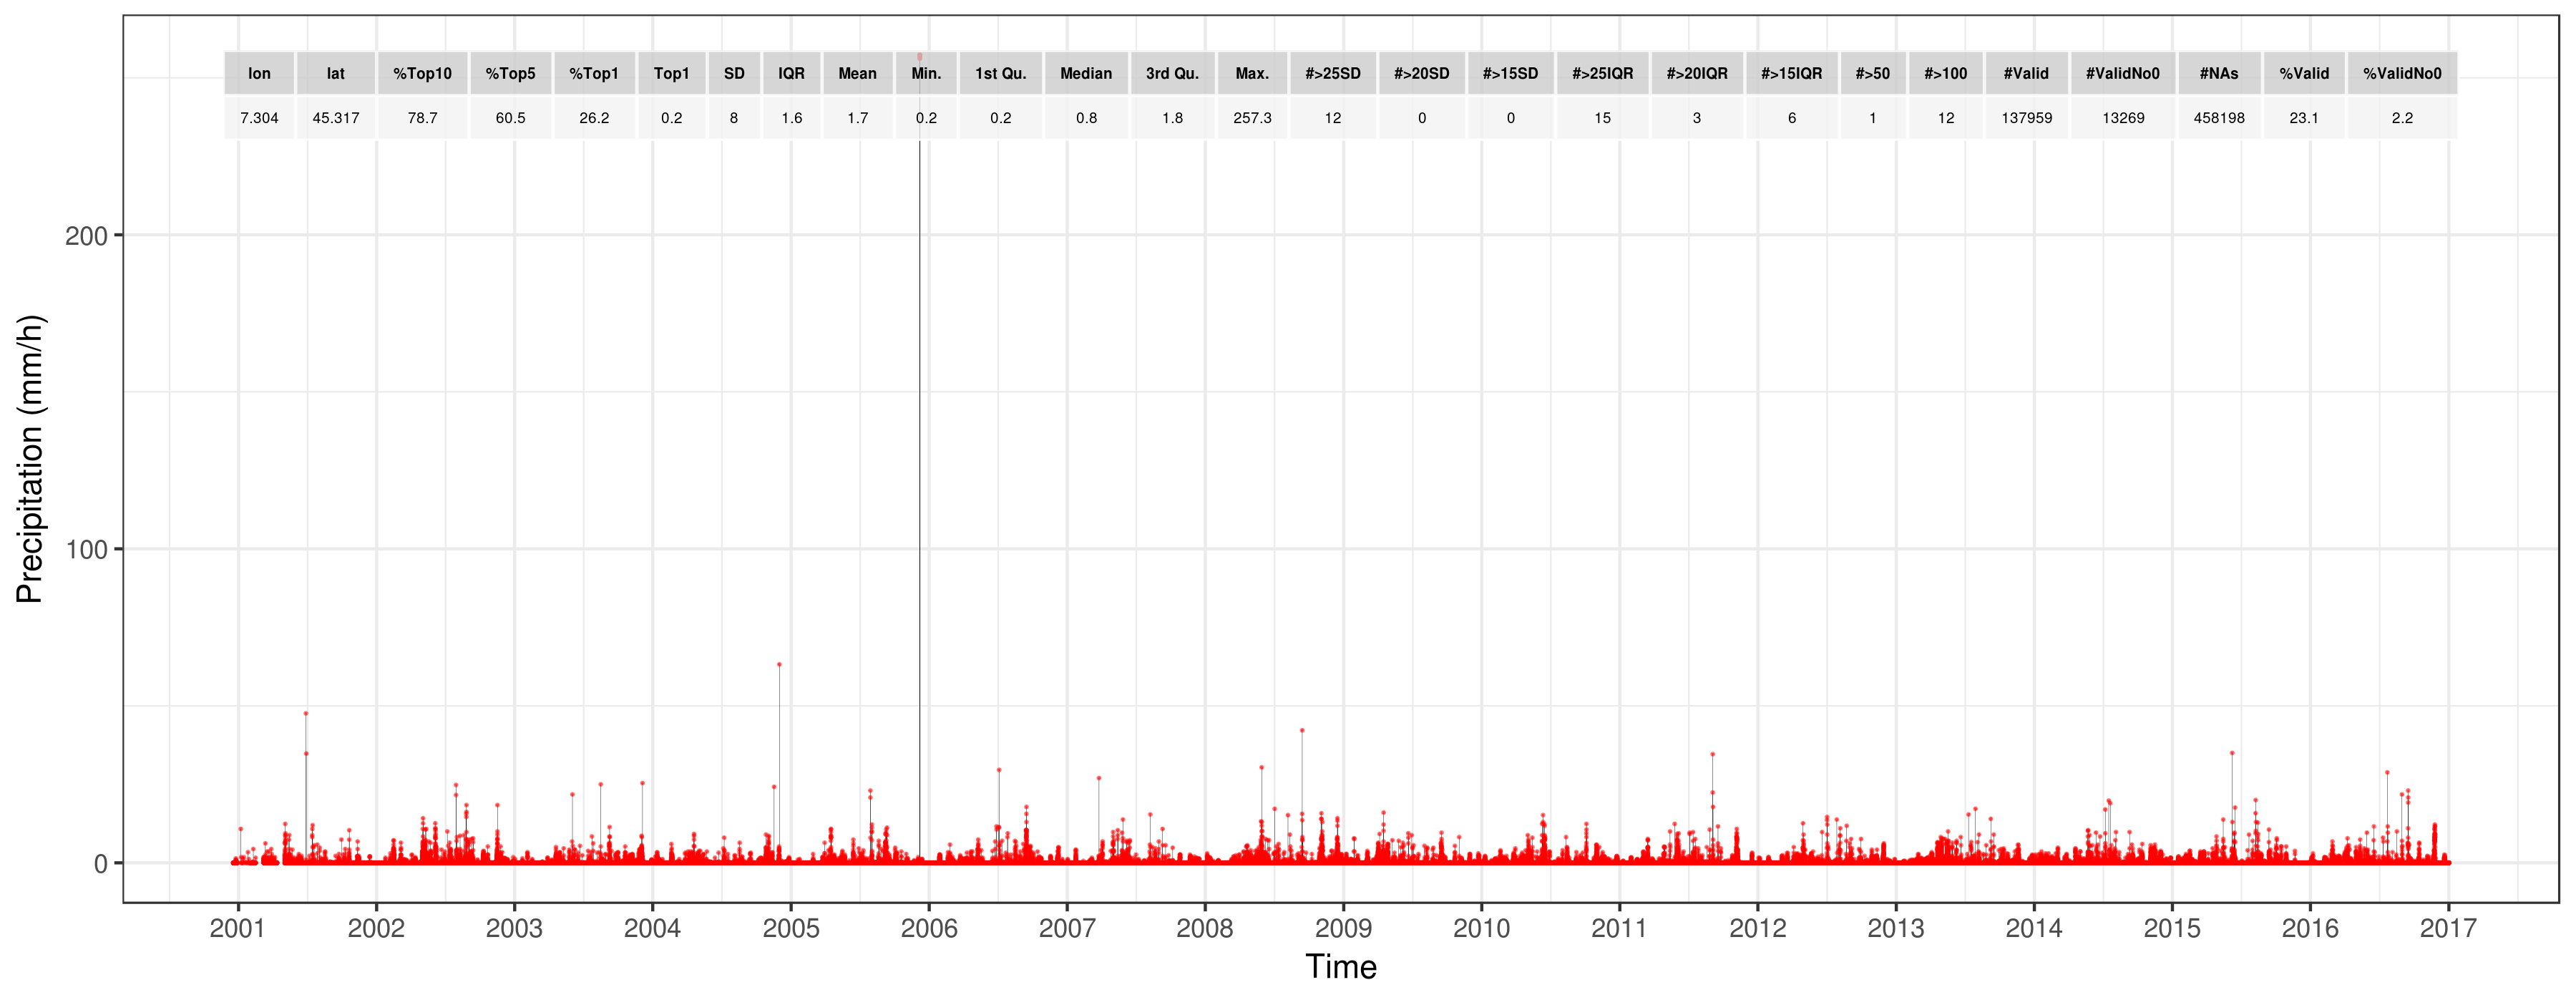
\includegraphics[width=\textwidth]{figures/rain_dst/16_ts.png}
    \end{subfigure}\\
    \begin{subfigure}{\textwidth}
        \caption{}\label{fig:ts_rain/c}
        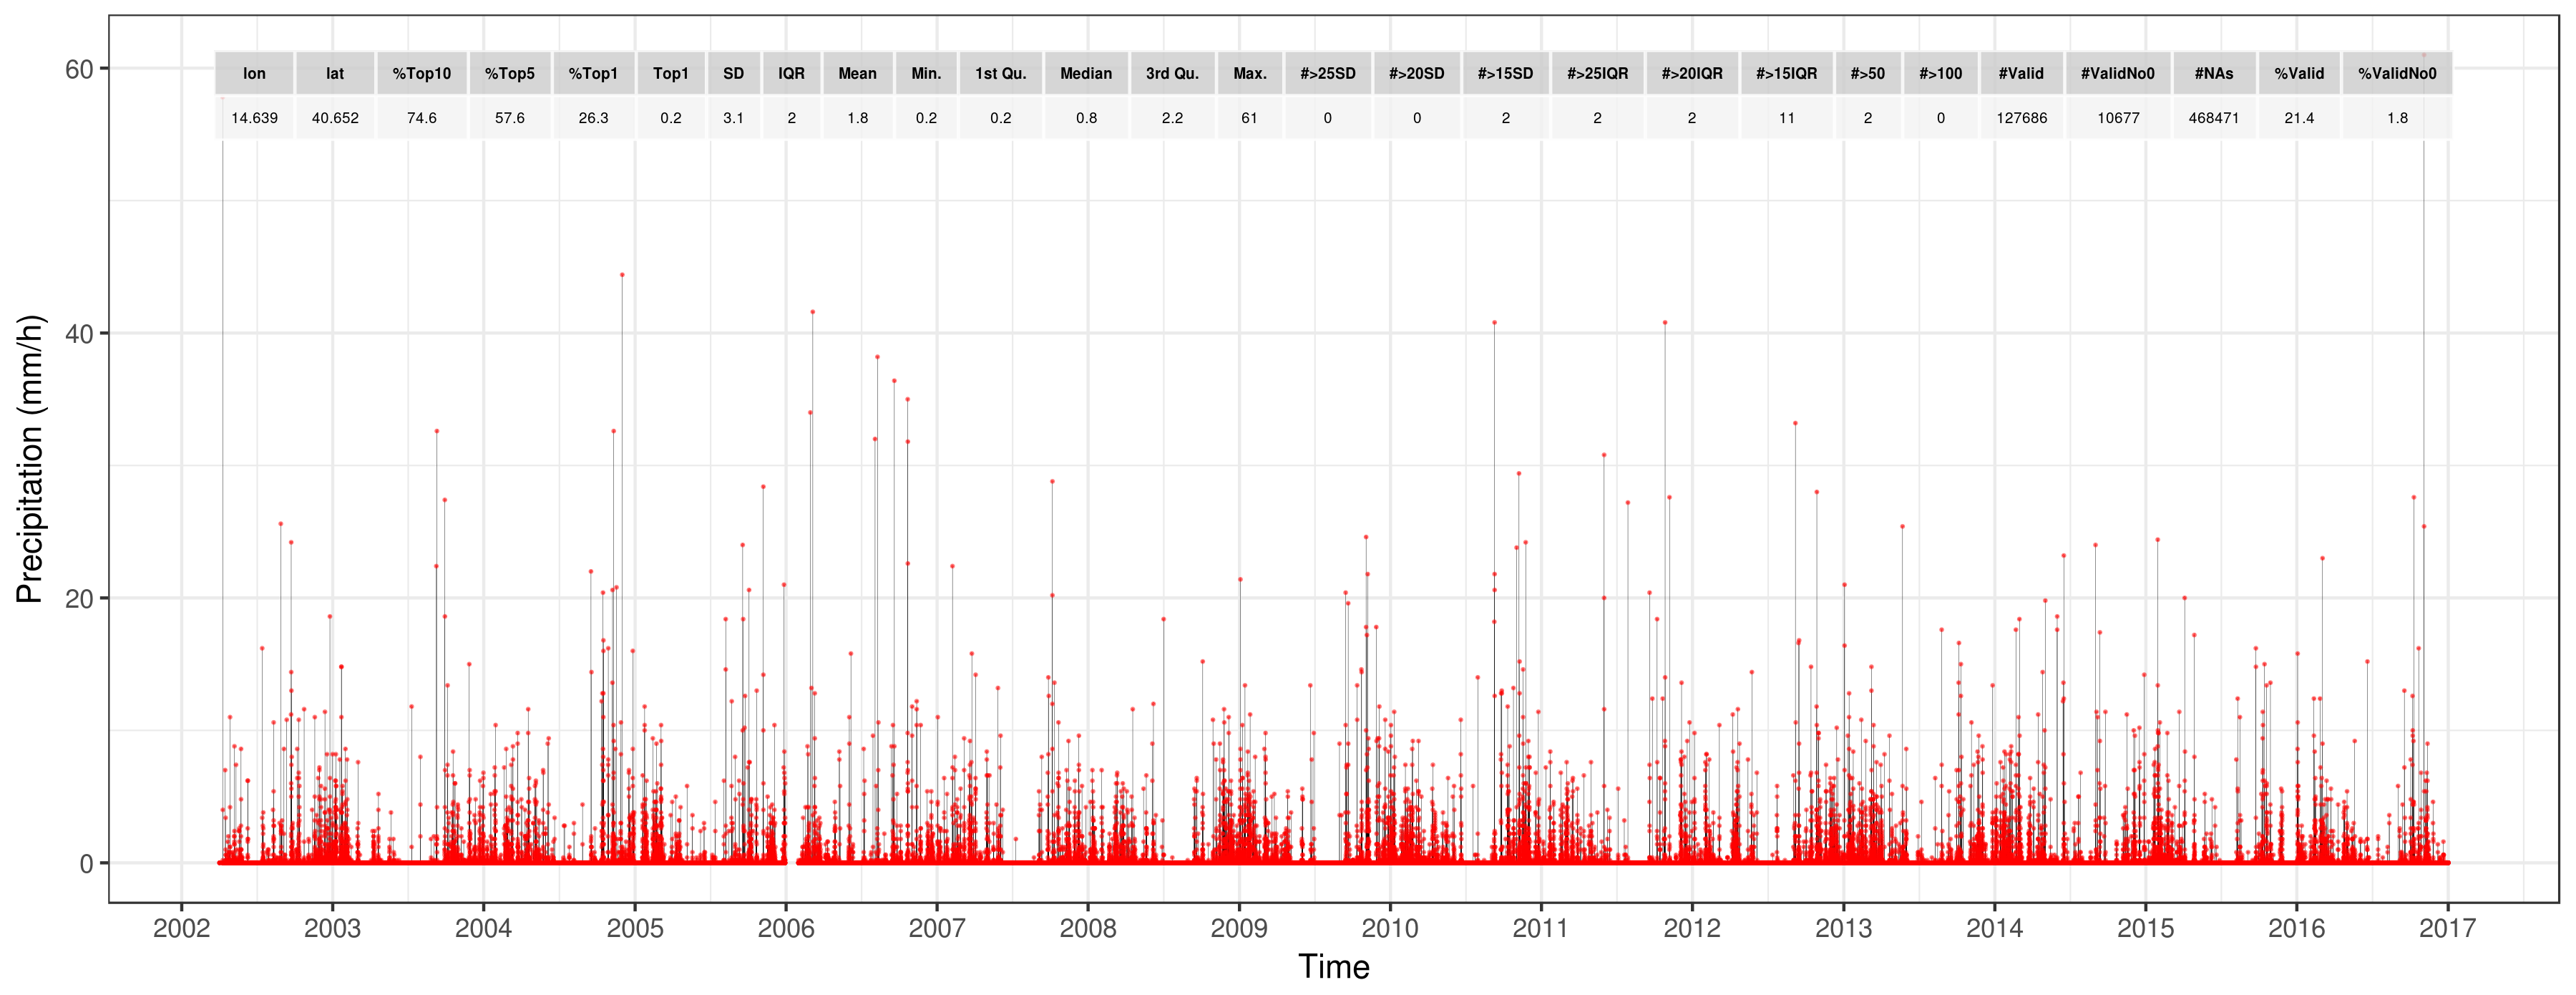
\includegraphics[width=\textwidth]{figures/rain_dst/613_ts.png}
    \end{subfigure}
    \decoRule
    \caption[Example precipitation timeseries from station data]{Three example precipitation timeseries from stations located in (top to bottom) Arienzo (Naples), Ala di Stura (Turin) and Maiori (Salerno). In panel \subref{fig:ts_rain/a}, the continuous zero values in 2003 indicate a stuck sensor. In panel \subref{fig:ts_rain/b}, a clear outlier at the end of 2005 can be considered an instrumental fluke with high certainty, due to the extremely high value above historical records. Panel \subref{fig:ts_rain/c} instead shows a station remarkable for its consistency and quality. Tables with some of the statistics computed for each station are also shown at the top of each panel.} \label{fig:ts_rain}
\end{figure}

To mitigate these problems, a multi-step approach of manual checking, driven by different metrics, is devised, comprising of \ref*{enum:steps_last} different steps:
\begin{enumerate}
    \item Flagging of suspicious events using several metrics obtained from the literature \citep{WMO2008}. The description of the metrics can be found in \cref{tab:flags_descr}. \label{enum:steps_1}
    \item Identification of values above the historical maxima for the region of interest, which are considered erroneous and removed. Three different thresholds are used, one for hourly values (\SI{200}{\milli\metre\per\hour}), one for monthly sums (\SI{1800}{\milli\metre\per\month}), and one for extreme step changes with the previous/next timestep (\SI{100}{\milli\metre\per\hour}). If these thresholds are exceeded more than 100 times in any given year, the entire year is removed. This filtering are carried out by the data provider, Marco Verdecchia, on the original binary data. \label{enum:steps_2}
    \item Second flagging of the values identical to step \ref{enum:steps_1}, to verify changes after the filtering occurred in \ref{enum:steps_2}. The results, shown in \cref{tab:flags_res}, show that the vast majority of suspicious values are removed after the initial cleaning procedure. In particular, 99.7\% of precipitation events above \SI{100}{\milli\meter\per\hour} are found to be unrealistic; the reduction drops to 76.3\% for events between 50 and \SI{100}{\milli\meter\per\hour}.
    In total, 82.1\% of the total flags are removed by applying this simple technique.
    \item Visualisation and selection of problematic months for each station using some of the metrics of point \cref{enum:steps_1}, aggregated on monthly scale and displayed via 192 (16 years $\times$ 12 months) interactive web maps (\cref{fig:clean_dewrain_screenshot,fig:ts_dewrain_example}), in which suspicious stations for each month are manually compared with their neighbours and, if considered unreliable, removed. \label{enum:steps_last}
    % ***TODO*** this figure should be updated with the line after the SECOND stage filtering!
\end{enumerate}
As a result of this cleaning process, the reduction in the total number of valid data points results to be modest and especially concentrated in the last few years (\cref{fig:filVSnofil_station_count_line}). A brief overview of the improvement on the data quality obtained thanks to these simple procedures will be presented in \cref{sec:valid_itaobs}.
\begin{figure}
    \centering
    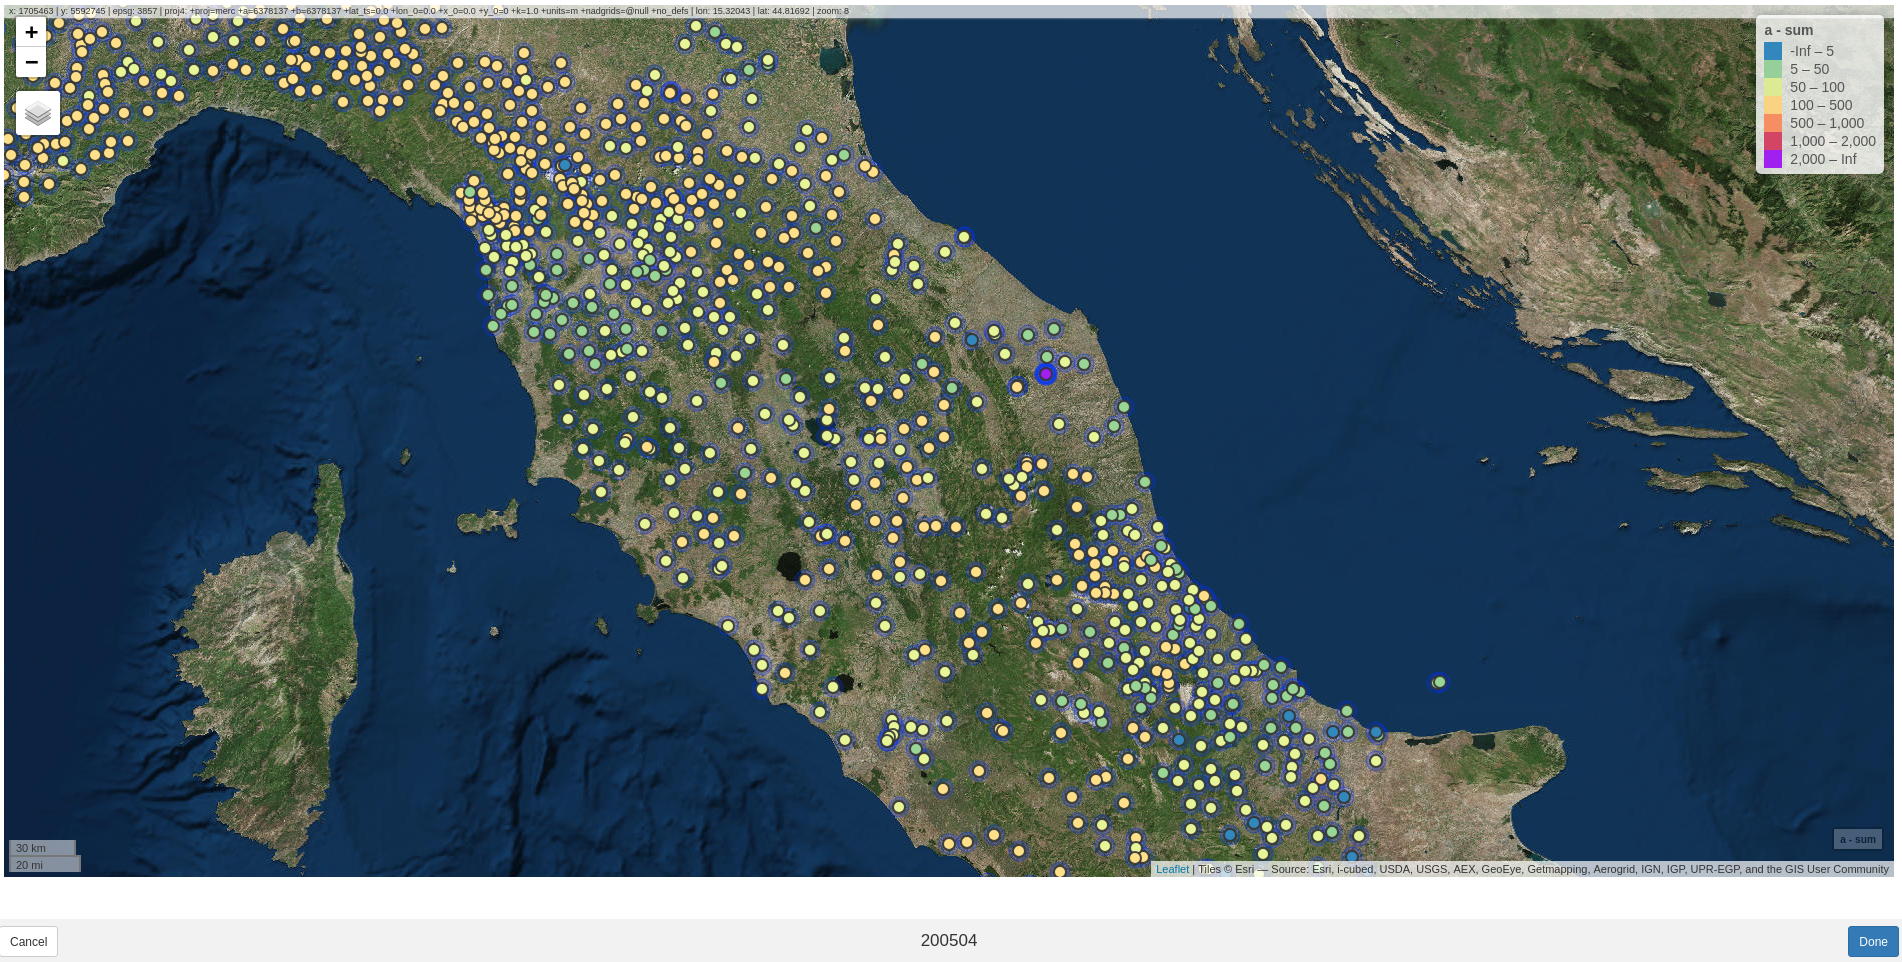
\includegraphics[width=\textwidth]{figures/rain_dst/clean_dewrain_screenshot}
    \decoRule
    \caption[Manual cleaning procedure for the precipitation dataset  GRIPHO]{Example screenshot of one of the steps in the manual cleaning procedure for the hourly precipitation dataset GRIPHO. Here, for each month, stations are plotted on an interactive map coloured by their total precipitation amount. Clicking on a station pops up a timeseries plot for that station (\cref{fig:ts_dewrain_example}), so that several neighbouring stations can be easily compared; clicking the blue circle surrounding a station selects it for exclusion from the dataset.} \label{fig:clean_dewrain_screenshot}
\end{figure}
\begin{figure}
    \centering
    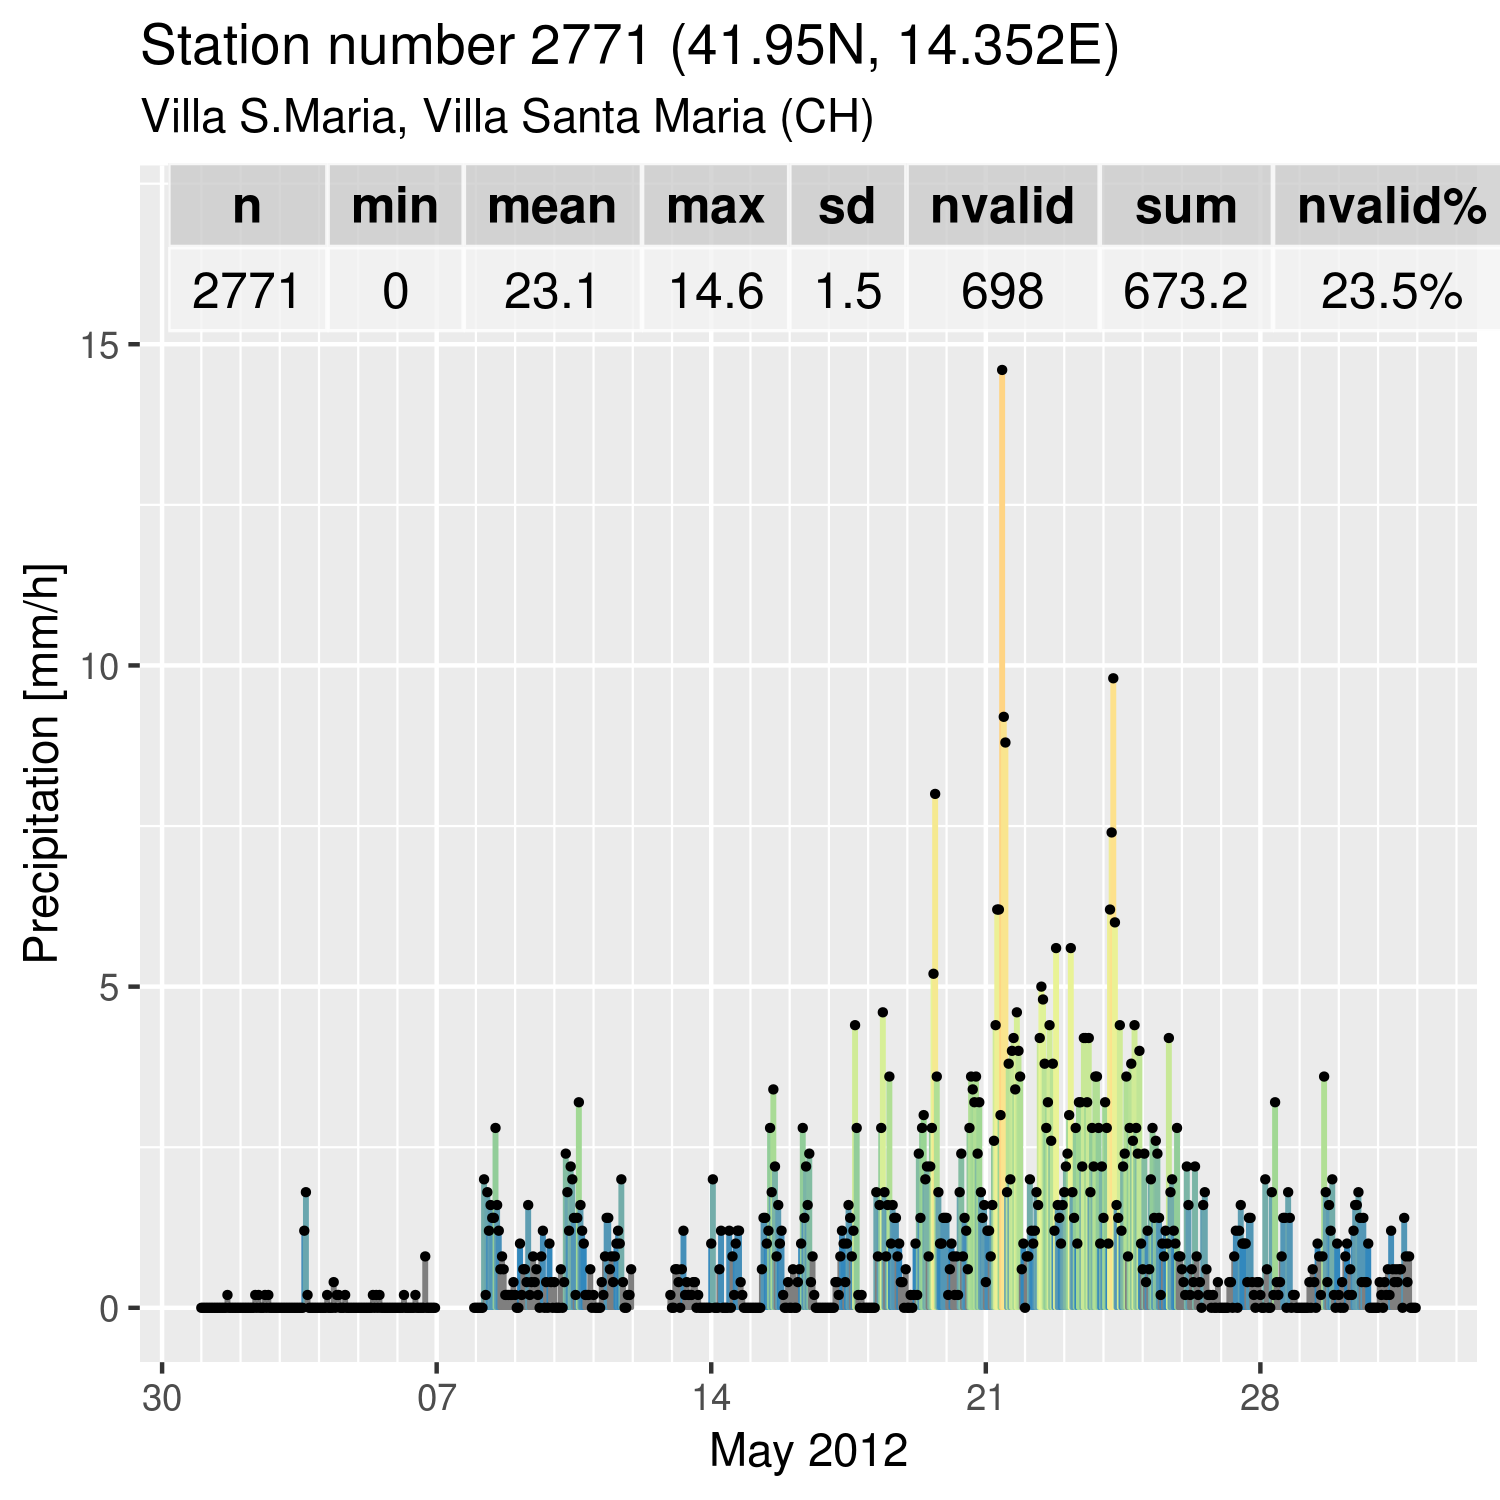
\includegraphics[width=\textwidth]{figures/rain_dst/ts_dewrain_example}
    \decoRule
    \caption[Example timeseries popup for the cleaning of the precipitation dataset GRIPHO]{Example precipitation timeseries for May 2012 for a station in Southern Italy. Graphs like this are used to compare neighbouring stations in the procedure of \cref{fig:clean_dewrain_screenshot}. About 360000 of these graphs were generated.} \label{fig:ts_dewrain_example}
\end{figure}

\begin{table}
\centering
\begin{tabularx}{\textwidth}{lX}
\toprule
Metric                                   &
                                         Meaning \\ \midrule
Total valid values                       &
                                         Number of values in the whole time series which are not one of the strings considered NA or negative \\
pr \textgreater{} Mean + \emph{n}SD      &
                                         Number of values greater than \emph{n} standard deviations from the mean; $n=10,15,20$\\
pr \textgreater{}  Median + \emph{n}IQR  &
                                         Number of values greater than \emph{n} interquartile ranges from the median; $n=10,15,20$   \\
100 \textgreater{}  pr \textgreater{}  50 mm/h &
                                         Number of values greater than \SI{50}{\milli\metre\per\hour}, but smaller than \SI{100}{\milli\metre\per\hour} \\
pr \textgreater{} 100 mm/h               &
                                         Number of values greater than \SI{100}{\milli\metre\per\hour} \\
\%Top \emph{n}                           &
                                         Percentage of values among the top \emph{n} most common values, excluding 0; $n=1, 5, 10$ \\
\% valid values                          &
                                         Total percentage of valid values \\
\% valid values $\neq$ 0                    &
                                         Total percentage of valid values which are not equal to 0 \\
\end{tabularx}
\decoRule
\caption[Description of all used metrics for suspicious values]{Description of all the metrics used for flagging suspicious values before and after the first automated cleaning procedure, and for selecting complete months to remove in the last manual process.}
\label{tab:flags_descr}
\end{table}

\begin{table}[]
\centering
\begin{tabular}{@{}llll@{}}
\toprule
Metric                                   & Original & Filtered & \% change \\ \midrule
Total valid values                       & 250M     & 244M     & -2,6\%    \\
Total flags                              & 324468   & 58008    & -82.1\%   \\
pr \textgreater{} Mean + 20SD              & 3240     & 2538     & -21.7\%   \\
pr \textgreater{} Median + 20IQR           & 49753    & 22519    & -54.7\%   \\
100 \textgreater{} pr \textgreater{} 50 mm/h & 21758    & 5171     & -76.3\%   \\
pr \textgreater{} 100 mm/h                 & 221822   & 711      & -99.7\%       
\end{tabular}
\decoRule
\caption[Metrics for suspicious values before and after automatic first stage filtering]{Selected metrics for suspicious values before and after automatic first stage filtering. See \cref{tab:flags_descr} for a description of all metrics.}  \label{tab:flags_res}
\end{table}

\begin{figure}
    \centering
    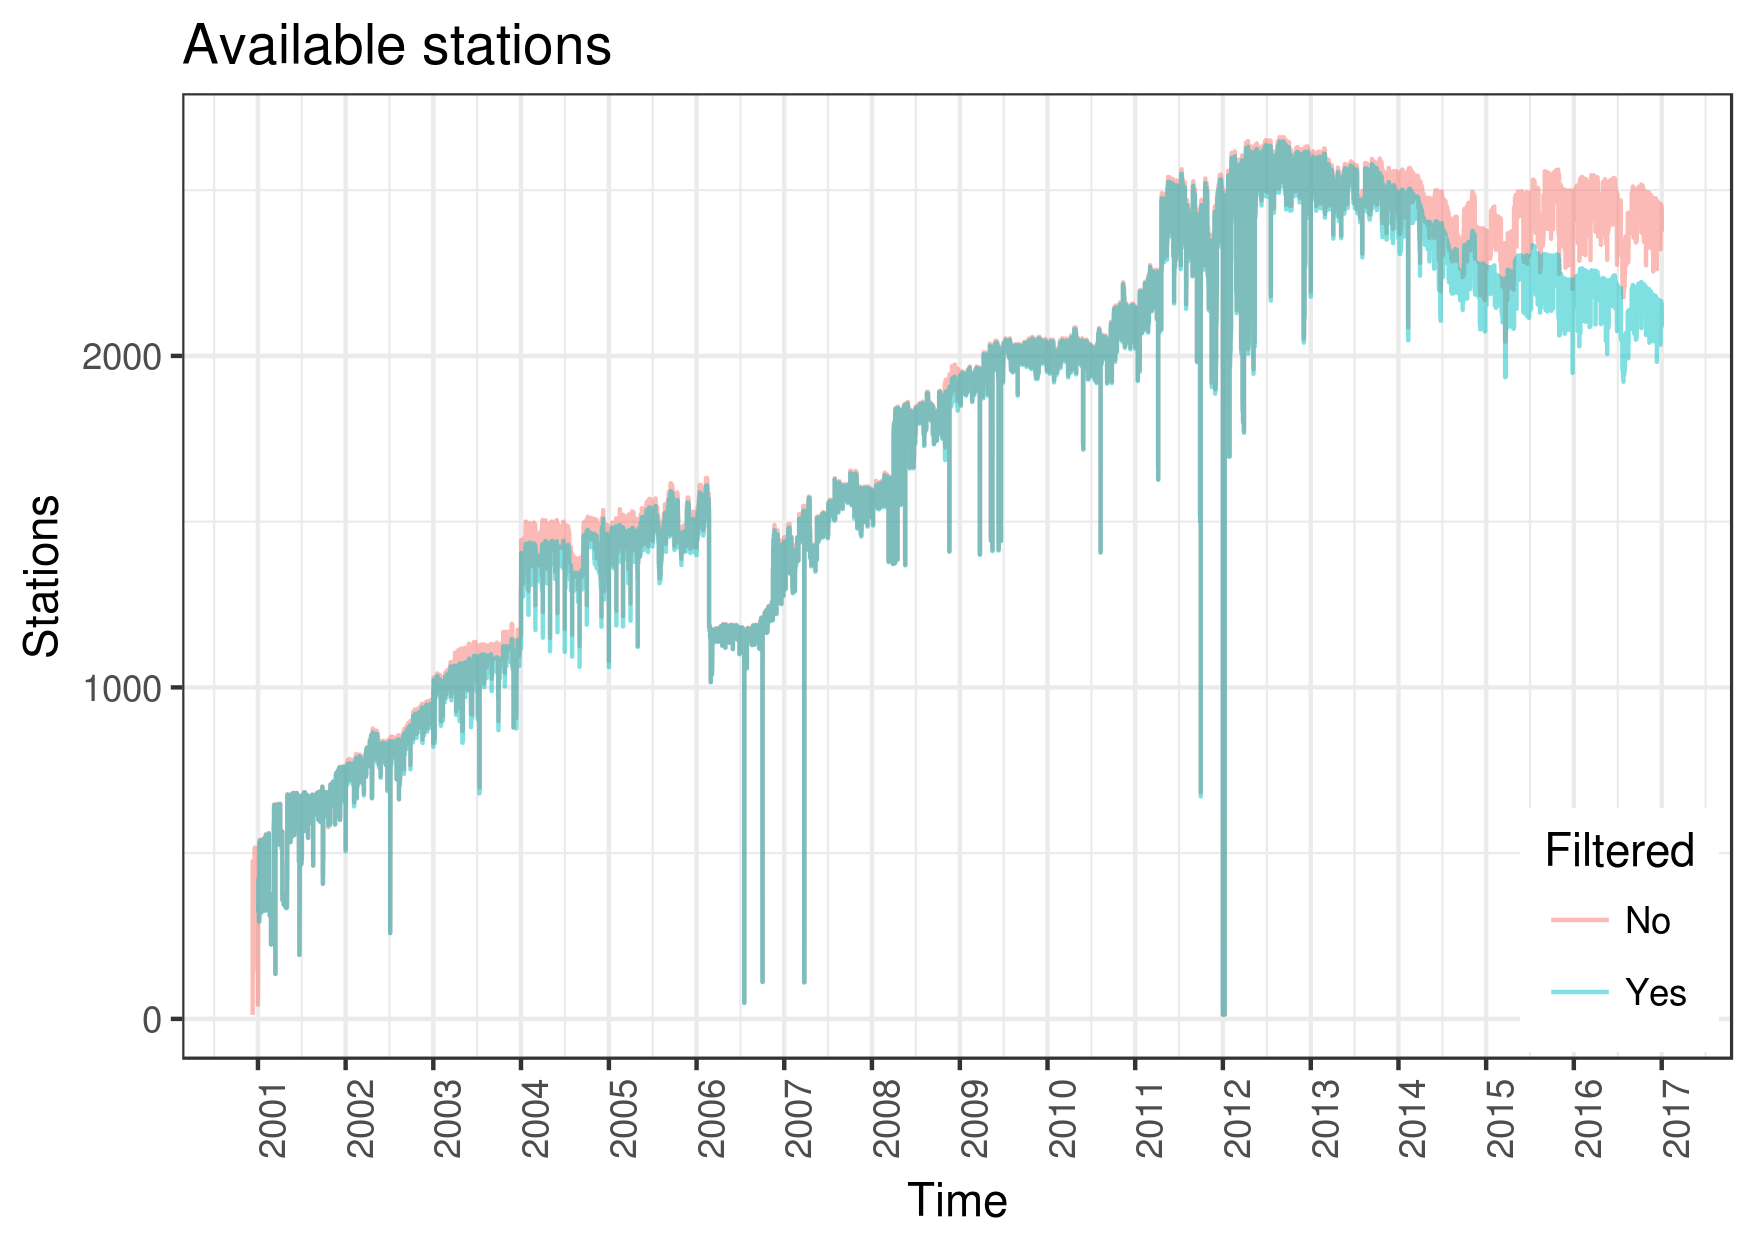
\includegraphics[width=\textwidth]{figures/rain_dst/filVSnofil_station_count_line}
    \decoRule
    \caption[Count of available stations per timestep, filtered and non-filtered]{Timeseries of the number of available stations for each timestep in the input data for the Italian in-situ dataset, before and after the first-stage filtering.} \label{fig:filVSnofil_station_count_line}
\end{figure}


%------------------------------------
%	GRIDDING
%------------------------------------
\section{Gridding and output format}\label{sec:gridding}
To be able to compare the precipitation data with other similar products and with models, interpolating the station point data onto a grid is a necessary step.
Our first approach to this issue uses a simple interpolation method; different techniques are currently being tested.
The upcoming sections consist of a general view of the challenges that had to be faced, and the technical choices that were consequently made, while gridding the precipitation dataset described in this chapter.

\subsection{Overview of gridding techniques}\label{sec:gridding_techniques}
The interpolation of sparse data is a vast topic, with tens of different methods available, each with its own advantages and disadvantages.
There is no general consensus on which is the best method for precipitation, which is particularly difficult to treat due to the extremely local aspect of the phenomena, both in time and in space (this is especially true in summer, when most precipitation is of convective nature).
The precipitation datasets available over Europe (including those in \cref{tab:prec_obs_ita}) use a plethora of different gridding techniques, some of which are listed in the following.\\

The de-facto standard E-OBS dataset \citep{Haylock2008} uses a three step process: daily anomalies are applied with kriging over a monthly field obtained by spatial splines, taking into account the station elevation for the monthly averages.
The high-resolution EURO4M-APGD Alpine dataset \citep{Isotta2014} opts for a similar approach with a base field calculated with an adapted PRISM method \citep{Daly1994,Schwarb2001} and daily values obtained via a modified version of the SYMAP algorithm, which is a form of inverse distance weighting \citep{Shepard1984};
this algorithm \citep[adapted by][]{Antolini2016} is also used to produce the ARCIS dataset \citep{Pavan2018}.
KLIMAGRID \citep{Mohr2008,Mohr2009} instead chooses an approach based on Delaunay triangulation, in order to minimise smoothing at station points and keep extremes intact.
The HYRAS \citep{Rauthe2013} high-resolution dataset over Germany uses the REGNIE method \citep{Weerts2008}: for each different climatological area, mean fields and climatologies are calculated using least-squares multiple linear regression (against location, slope, height and exposition) and inverse distance weighting.
The Austrian dataset SPARTACUS \citep{Hiebl2017} calculates a base field with kriging and topographic predictors, to which SYMAP daily anomalies are applied.

To our knowledge, there is limited literature comparing the performance of these interpolation methods for high-resolution gridded precipitation data. A general validation was carried over by \citet{Hofstra2008}, which ultimately resulted in the choice of interpolation technique for the E-OBS dataset mentioned above.

\subsection{The chosen spatial grid}
The choice of grid is dictated by station density and convenience. With an average station spacing of about \SI{10}{\kilo\meter}, the grid choice fell on the \SI{12}{\kilo\meter} EURO-CORDEX one used by the Regional Climate Model RegCM. The resulting $95 \times 110$ grid (\cref{fig:rain_dst_grid}) has a constant grid spacing of \SI{12}{\kilo\meter} on a Lambert Conformal Conic projection. Unlike more common regular latitude-longitude grids, using a curvilinear grid preserves constant grid cell areas, which simplifies later calculations.

\begin{figure}
    \centering
    \includegraphics[width=0.7\textwidth]{figures/rain_dst/rain_dst_grid}
    \decoRule
    \caption[Grid for the hourly rain dataset GRIPHO over Italy]{Grid of the hourly rain dataset GRIPHO over Italy, projected over Esri\copyright \ World Imagery tiles in Mercator projection (EPSG code 3857).} \label{fig:rain_dst_grid}
\end{figure}

\subsection{Gridding procedure}
In this work, due to technical constraints, a simple interpolation technique (which minimises the smoothing of extreme phenomena) is chosen to regrid the cleansed station data obtained after the manual and automatic filtering steps seen in \cref{sec:data_cleaning}\footnote{
    The regridding software was adapted for use on this project from a program provided by Graziano Giuliani from Earth System Physics (ESP) section of the International Centre for Theoretical Physics (ICTP), who also helped at various stages of this project with general software consulting. Graziano's help was irreplaceable and greatly appreciated.
}.\\ 
The method is based on SciPy's \citep{Jones2007} \texttt{interpolate.griddata}, which employs the Qhull library\footnote{\url{http://www.qhull.org}} \citep{Barber1996}. 
Both the linear and the cubic variant were taken into consideration, but since no significant climatological difference was found between the two methods, the linear version was employed.
This method performs a Delaunay triangulation \citep{Aurenhammer1991} on all the available points separately for each timestep, creating a grid of triangular cells whose corner values are linearly interpolated to evaluate the cell values on the underlying rectangular grid.
In this sense, this procedure is similar to the works of \citet{Velasquez2011,Mohr2008}, which also used Delaunay triangles to perform interpolation of sparse rainfall data sources.
An example Voronoi diagram associated to the Delaunay triangulation of the timestep containing the highest number of stations is showed in \cref{fig:voronoi}.
\begin{figure}
    \centering
    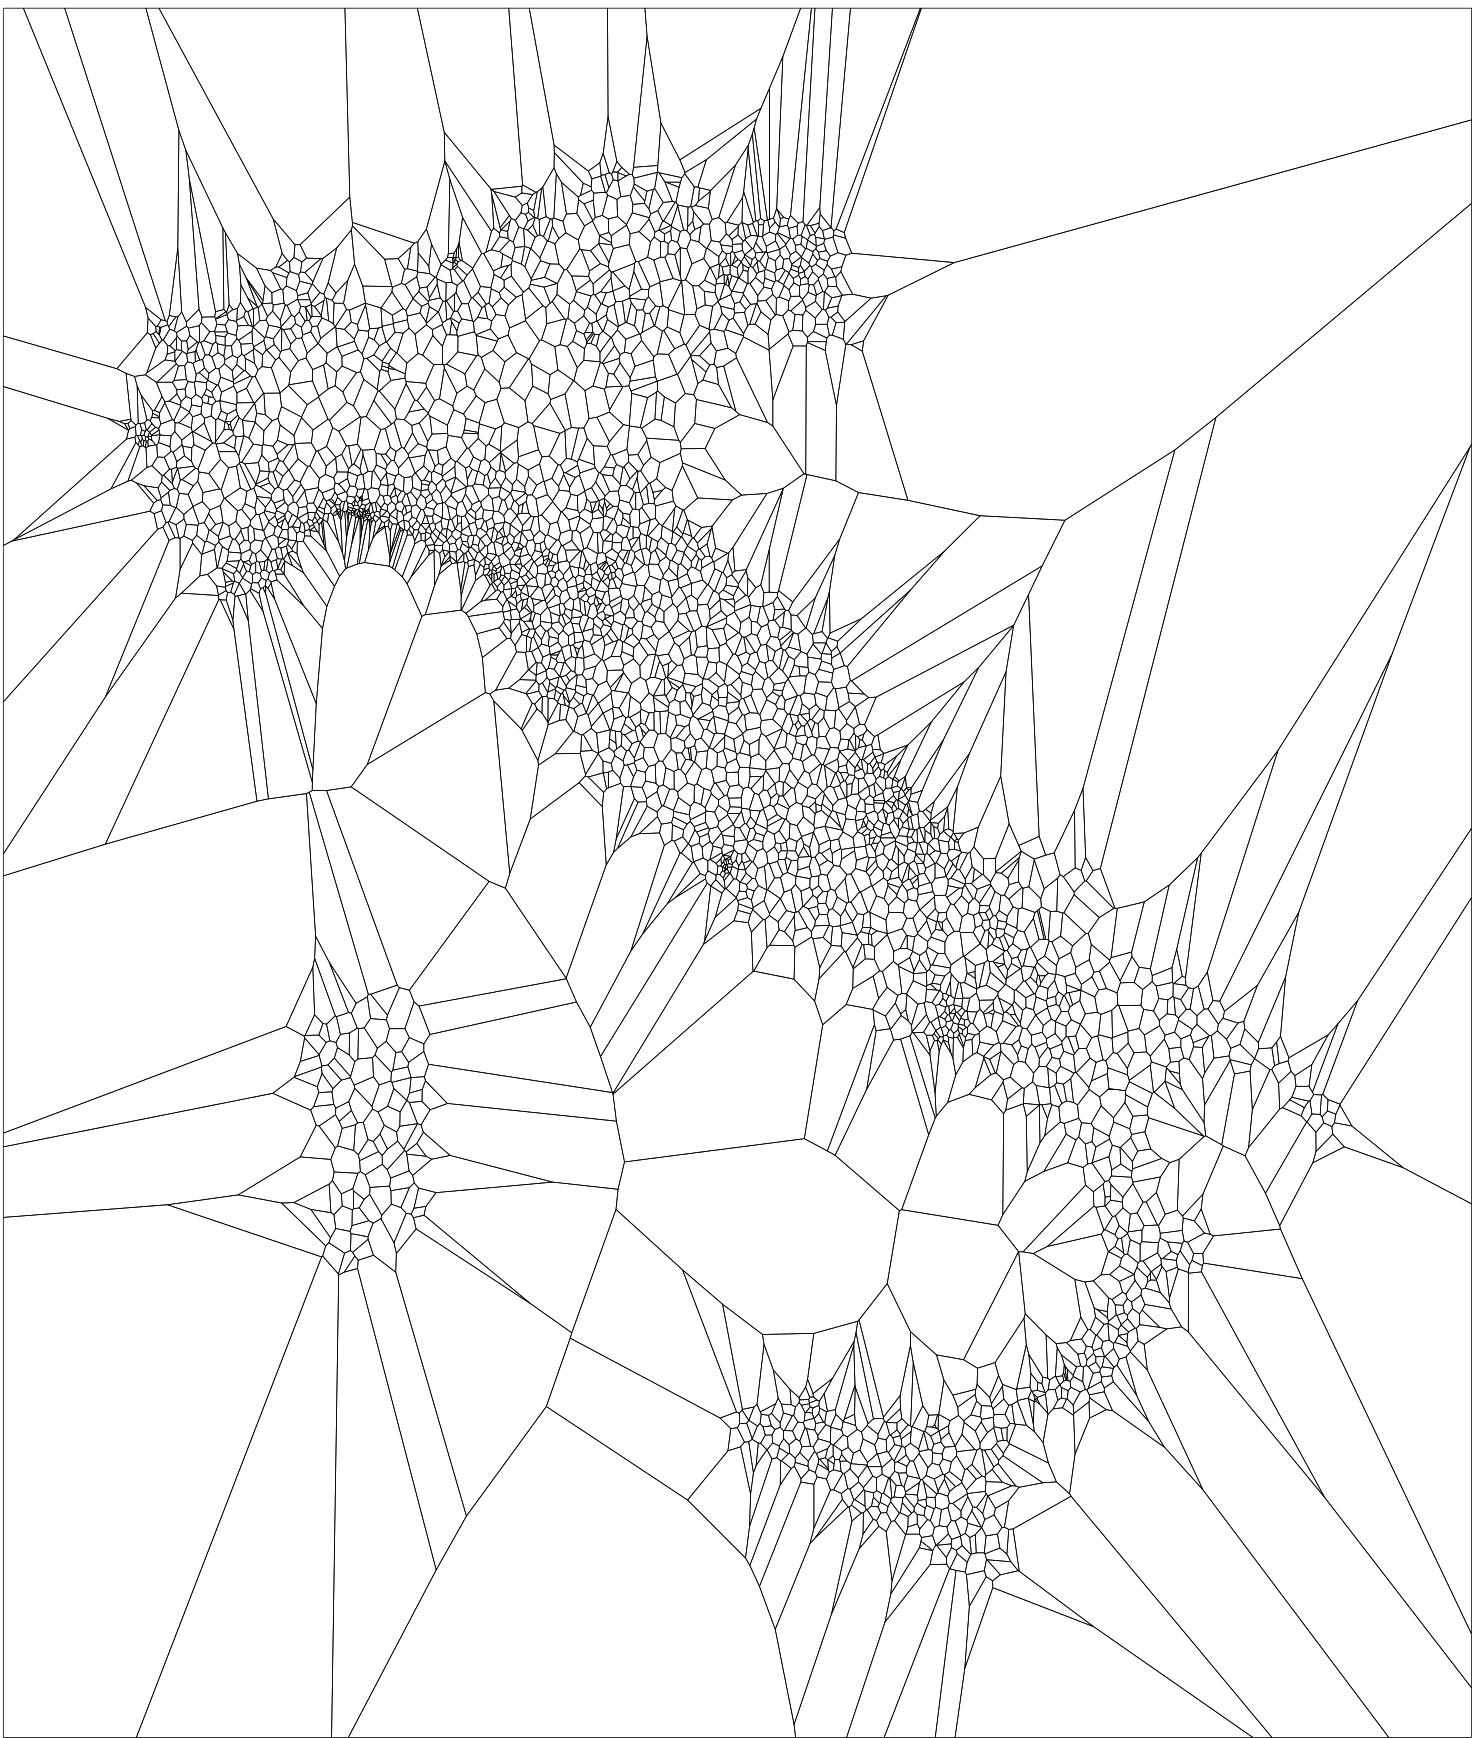
\includegraphics[width=0.7\textwidth]{figures/voronoi}
    \decoRule
    \caption[Example Voronoi diagram for the creation of the precipitation dataset GRIPHO]{Voronoi diagram corresponding to the Delaunay triangulation  of all stations. Example given for the timestep with the highest number of valid stations for the gridded Italian station-based precipitation dataset GRIPHO.} \label{fig:voronoi}
\end{figure}
After the interpolation, values over the sea are forcefully set to missing.
The result of the interpolation is, of course, more reliable for periods and regions with high station density; for this reason regions with low station density are also set to missing during the interpolation procedure.
This results in a dataset which can have both spatial and temporal empty zones, which is similar to what other station-based datasets have \citep[the E-OBS dataset from][for example, also has varying missing values]{Hofstra2008}.
The interpolation was separately carried out in parallel for each time slice, with no information crossing time boundaries.
\Cref{fig:gridVSnogrid_pdf} shows the Probability Density Function of GRIPHO in its gridded and non-gridded (raw) form: as expected, gridding introduces a general smoothing of precipitation extremes. The effect is however quite small, thanks to the choice of interpolation method, and most extreme events are retained.
Compared to most of the techniques seen in \cref{sec:gridding_techniques}, this approach is much faster but also more basic; improving this method will certainly be the goal of future research.
Additional information on the interpolation methodology, including tests with different algorithms, are presented in \citep[][in preparation]{Fantini2018a}.

\begin{figure}
    \centering
    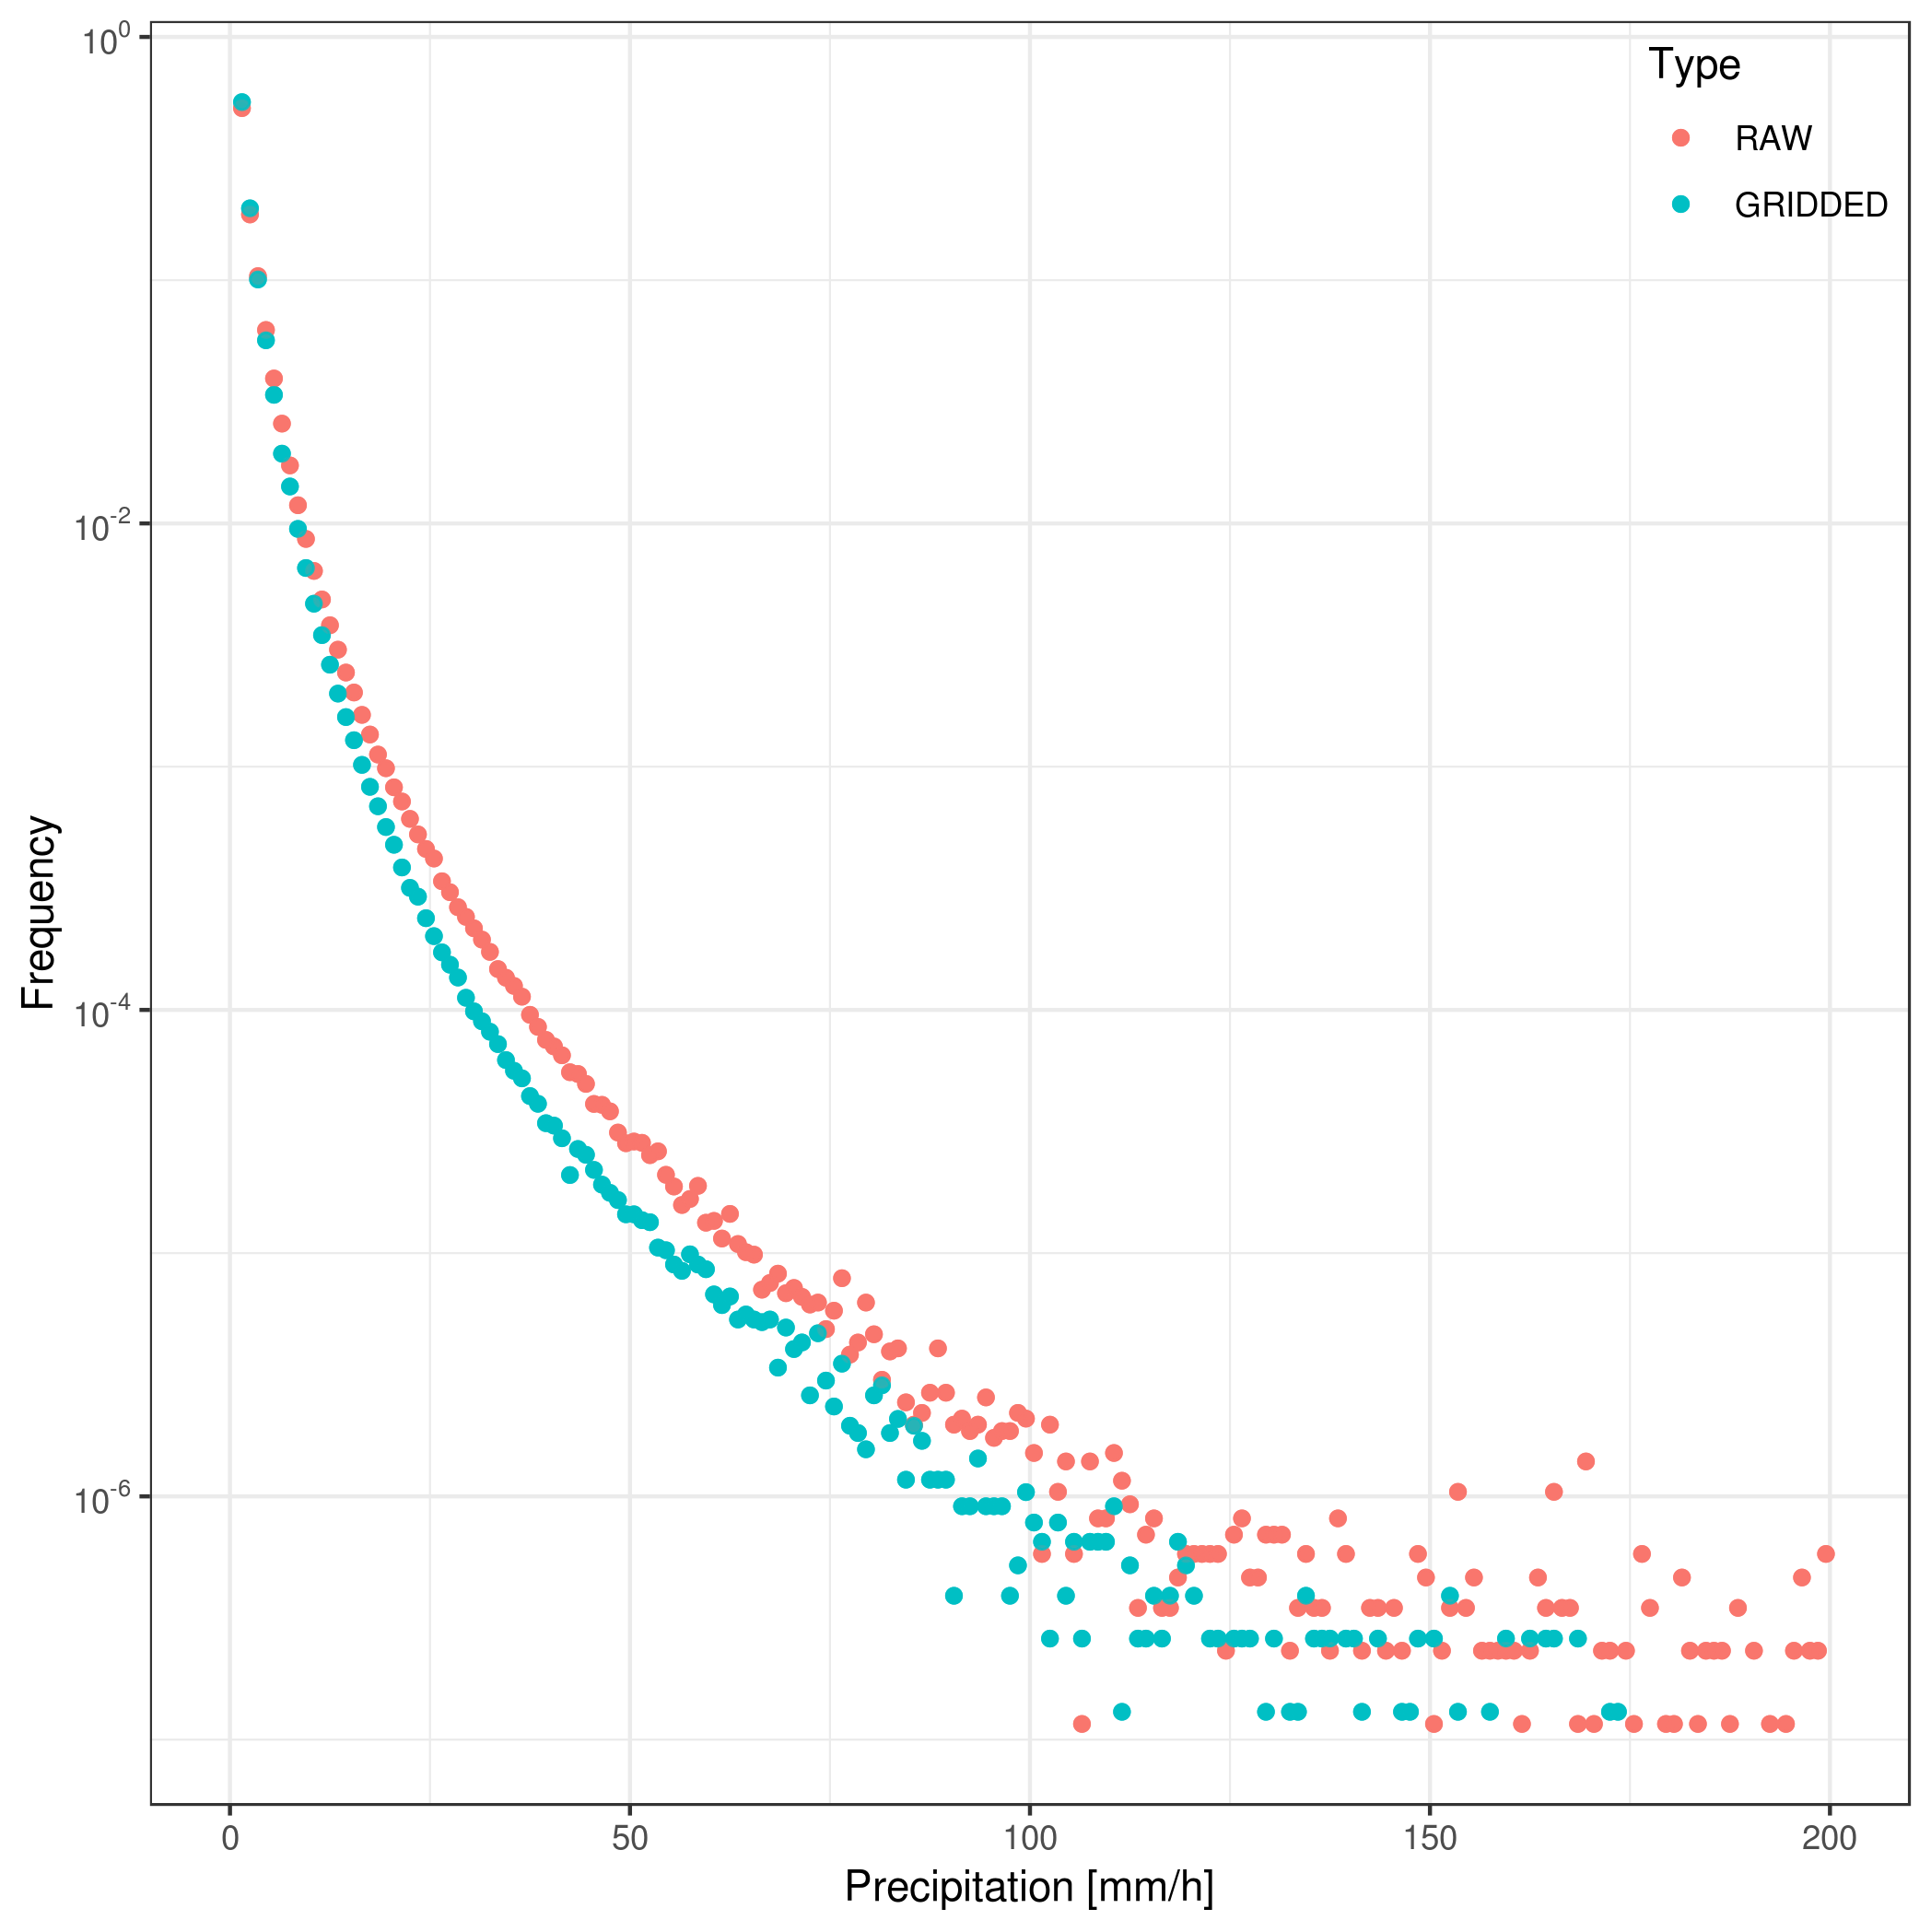
\includegraphics[width=\textwidth]{figures/rain_dst/validation/compare.png}
    \decoRule
    \caption[PDFs for gridded and raw station data for the Italian hourly precipitation dataset GRIPHO]{Comparison of the precipitation distributions from the gridded (teal) and raw (red) hourly precipitation datasets. As is to be expected, gridding introduces a general smoothing of precipitation extremes.} \label{fig:gridVSnogrid_pdf}
\end{figure}

\subsection{Output format}
Once again, the chosen output format is CF-compliant losslessly-compressed netCDF-4. The complete GRIPHO dataset resulted in 192 monthly files, for a total of 561021 quarter-hourly timesteps over the $95 \times 110$ grid. The total size of the dataset is \SI{647}{\mega B} when adding up the sizes of each separate month, or \SI{507}{\mega B} if considering a single aggregated file; the two sizes differ because of the higher compression efficiency resulting from compressing the single, larger file. For the aggregated file, the compression ratio, when compared to an uncompressed dataset, is 44$x$.\\
Due to the aforementioned low amount of sub-hourly values an additional, hourly dataset was created by aggregating sub-hourly data. This version has 140256 timesteps and is \SI{404}{\mega B} in size.

For ease of use and download, both these versions were also further compressed by applying a lossy procedure, reducing data precision to \SI{0.1}{\milli\meter\per\hour}. In these versions, the data is stored as short (16-bit) integers, instead of 32-bit floats; a CF-standard \texttt{scale\_factor} attribute indicates these are to be rescaled to floats when read. This further reduces the size of the dataset to \SI{248}{\mega B}, or \SI{184}{\mega B} for the hourly version.

An additional GRIPHO version, containing a variable optimised for reading along the time axis, one timeseries at a time, was also produced. These multiple versions should cover all possible needs and requirements of potential users, and exceed the technical standards usually followed in producing observational datasets for climate.

%------------------------------------
%	VALIDATION
%------------------------------------
\section{Validation against other precipitation datasets}\label{sec:valid_itaobs}
In this section, the new gridded hourly precipitation product presented in this chapter is validated against some of the datasets available over the Italian territory (see \cref{sec:obs_datasets,tab:prec_obs_ita}).
Only a basic validation is presented herein, further analysis is described in detail in \citet[][in preparation]{Fantini2018a}.

\subsection{Methodology and metrics}
Due to the lack of a suitable reference hourly dataset, the validation is carried out solely on the daily scale; analysis on the hourly scale is planned as a future research path.
As reported in \cref{sec:data_cleaning}, the GRIPHO dataset had several optimisations: in the following sections GRIPHO will be analysed both in its final form and in a version obtained after the first, automated cleaning (but without the subsequent manual procedures), in order to evaluate the effectiveness of these procedures.
In the figures, this version is referred to as ``Station (interp.)''\\
Four main metrics are presented here: annual cycle, mean seasonal precipitation, extreme seasonal precipitation ($\textrm{R95}_{ptot}$ and $\textrm{R99}_{ptot}$, see \cref{sec:uncertainty_pr}) and precipitation distribution (Probability Density Functions). Similarly to the analysis carried out in \cref{sec:uncertainty_pr}, annual cycles and PDFs are subdivided by region: North, Centre, South and Islands. Other than the product presented here, the datasets taken into consideration are EURO4M-APGD and ARCIS (only available in the North) and E-OBS and the HMR reanalysis (for the whole Italian territory). The nominal resolution of EURO4M-APGD, ARCIS and HMR is superior to that of GRIPHO. The ability to reproduce fine spatial details is however linked with station density: the EURO4M-APGD dataset, for example, is estimated to have an actual resolution of \SI{15}{\kilo\metre} or less \citep{Isotta2014}.
Similarly to \cref{sec:uncertainty_pr}, an observational period of 2000 to 2016 is considered, limited to 2008, 2013 and 2015 in the case of EURO4M-APGD, HMR and ARCIS respectively due to limited data availability.

\subsection{Results}
The annual cycle of precipitation (\cref{fig:valid_itaobs_pr_ac}) has a similar shape in all six datasets, with differences in precipitation intensity: E-OBS usually results the driest, and GRIPHO the wettest.
The filtering procedure of \cref{sec:data_cleaning} successfully removes a spurious peak in the August in the Islands, but has little to no impact on the average annual cycle of the other regions.\\
\Cref{fig:valid_itaobs_pr_mean} shows the spatial distribution of mean seasonal precipitation.
The spatial patterns and precipitation amounts in Northern Italy are remarkably similar to those from ARCIS and EURO4M-APGD.
In the other regions, GRIPHO results wetter than E-OBS and HMR, while showing similar spatial patterns with the latter.
The filtering process successfully removes some suspicious high precipitation values in Veneto (north-east, DJF) and  (centre-east, JJA), but does not filter out an excessive high value in the Southern tip of Sicily.
\begin{figure}
    % source of this data if you want to remake it:
    % /home/afantini/places/clima-archive4-b/regcm_simulations/EURO-CORDEX/validation/italy_validation/pr/
    \centering
        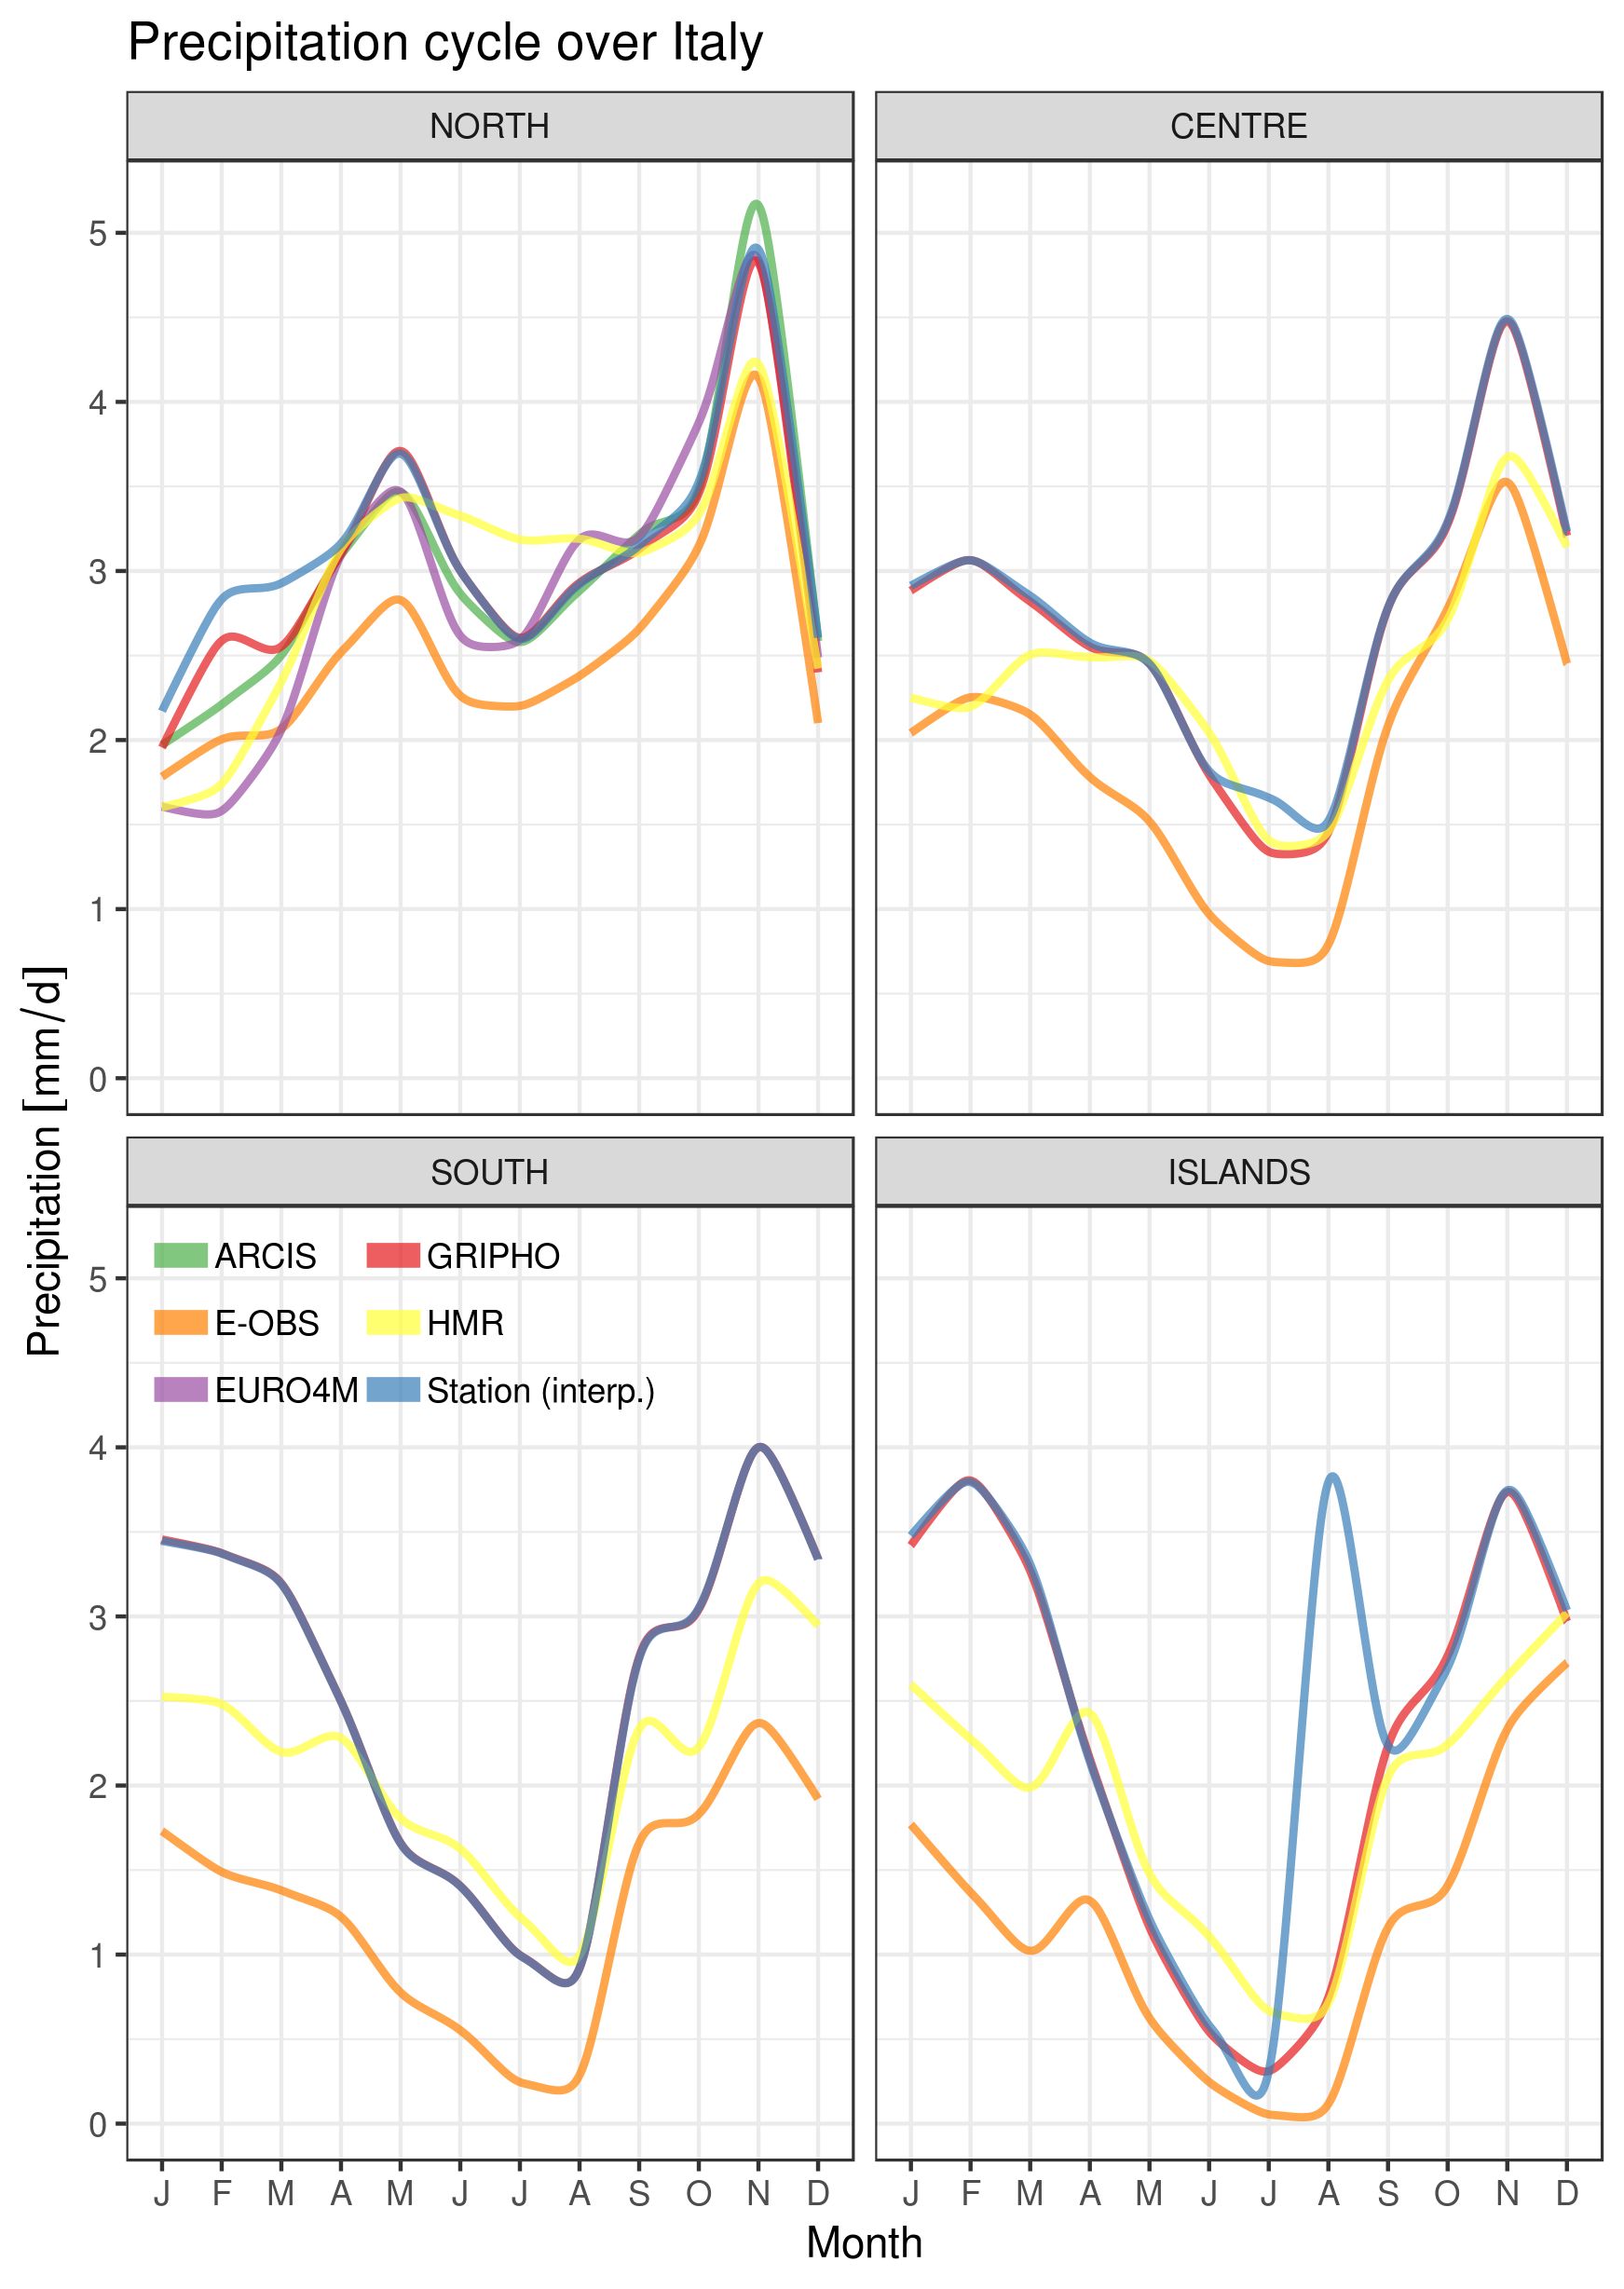
\includegraphics[width=0.7\textwidth]{figures/valid_itaobs/ac}
    \decoRule
    \caption[GRIPHO validation: annual cycle]{
        Average precipitation annual cycle for for the validation of the gridded hourly precipitation dataset. The four summarising regions are highlighted in \cref{fig:valid_itaobs_pr_mean,fig:valid_itaobs_pr_r95}.
} \label{fig:valid_itaobs_pr_ac}
\end{figure}
\begin{figure}
    \centering
        \includegraphics[width=0.7\textwidth]{figures/valid_itaobs/mean}
    \decoRule
    \caption[Validation of gridded hourly dataset: mean precipitation]{
        Average precipitation for the validation of the gridded hourly precipitation dataset. The four summarising regions for the annual cycle (\cref{fig:valid_itaobs_pr_ac}) and the PDFs (\cref{fig:valid_itaobs_pr_pdf1,fig:valid_itaobs_pr_pdf2}) are highlighted in green (North), red (Centre), purple (South) and blue (Islands).
} \label{fig:valid_itaobs_pr_mean}
\end{figure}

Extreme precipitation metrics (\cref{fig:valid_itaobs_pr_r95}, $\textrm{R99}_{ptot}$ not shown) once again show similar spatial patterns in the North compared with ARCIS and EURO4M-APGD and for the whole Italian region, especially compared with HMR especially.
Several extreme precipitation highs, such as the East coast of Sardinia in winter and parts of Calabria in autumn, are reproduced by both GRIPHO and HMR, but not as much by E-OBS.
The comparison of the first two rows of each plot shows that the manual filtering managed to significantly reduce what appears to be extreme precipitation excess in several areas, such as Abruzzo, Veneto, Valle d'Aosta, Sicily and Tuscany.
However, some extremes, most notably in Sicily and in Abruzzo, seem to have escaped the manual checking. For these, a second manual check will be necessary in a future version of GRIPHO.

The analysis of precipitation PDFs (\cref{fig:valid_itaobs_pr_pdf1,fig:valid_itaobs_pr_pdf2}) shows how GRIPHO contains more extreme events, compared to E-OBS and HMR, in all four regions. In the North, the difference with ARCIS and EURO4M-APGD is less striking, and all the datasets perform similarly, albeit GRIPHO seems to show some slightly more intense events than the ones in the other observational datasets.
Considering that none of these datasets include any kind of undercatch correction, this increase in extreme events is hard to evaluate.
This metric also shows very well how the filtering procedure significantly reduces the amount of extremely high precipitation events.
For the North, Centre and Isles the maximum amounts are decreased in all seasons, while no change is detected for the South of Italy.
\begin{figure}
    \centering
        \includegraphics[width=0.7\textwidth]{figures/valid_itaobs/r95ptot}
    \decoRule
    \caption[GRIPHO validation: $\textrm{R95}_{ptot}$]{
        Extreme $\textrm{R95}_{ptot}$ precipitation for the validation of the gridded hourly precipitation dataset. $\textrm{R95}_{ptot}$ represents the percentage of precipitation due to precipitation events above the 95th percentile.
} \label{fig:valid_itaobs_pr_r95}
\end{figure}
% \begin{figure}
%     \centering
%         \includegraphics[width=0.7\textwidth]{figures/valid_itaobs/r99ptot}
%     \decoRule
%     \caption[GRIPHO validation: $\textrm{R99}_{ptot}$]{
%         As \cref{fig:valid_itaobs_pr_r95}, but for $\textrm{R99}_{ptot}$.
% } \label{fig:valid_itaobs_pr_r99}
% \end{figure}
\begin{sidewaysfigure}
    \centering
        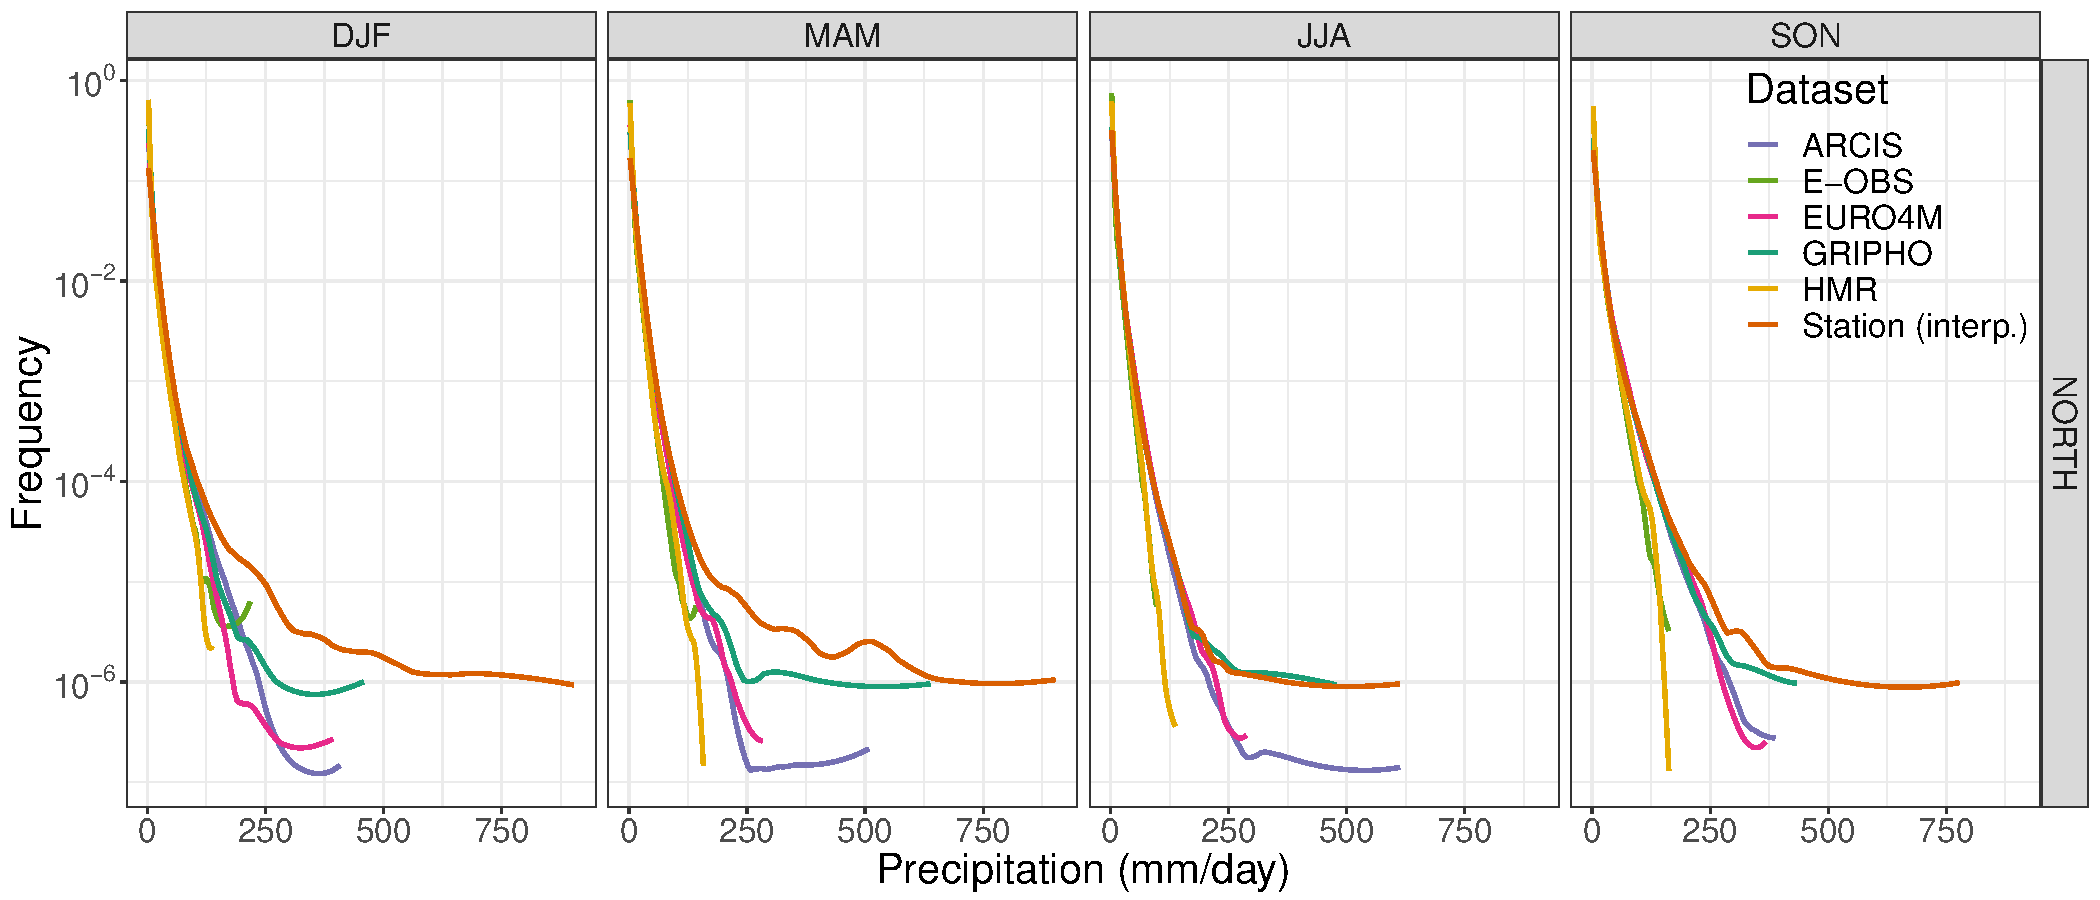
\includegraphics[width=0.8\textheight]{figures/valid_itaobs/pdf_NORTH_lines}
        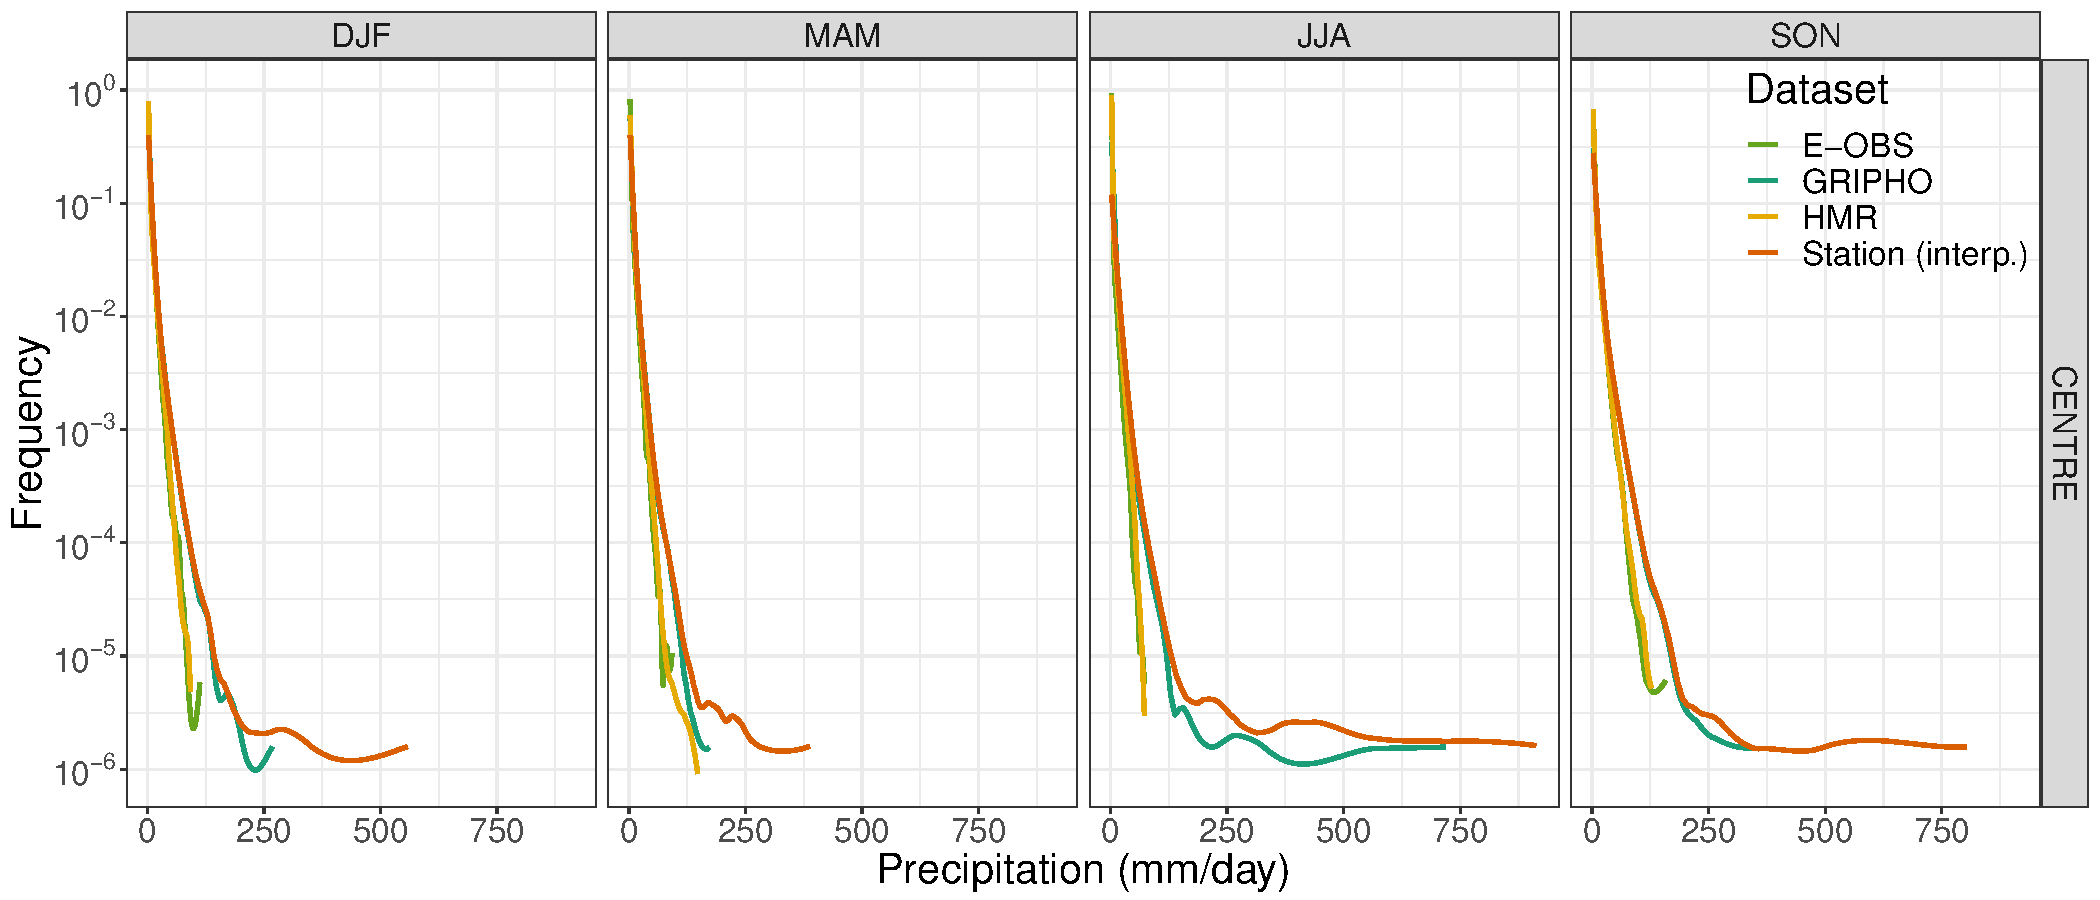
\includegraphics[width=0.8\textheight]{figures/valid_itaobs/pdf_CENTRE_lines}
    \caption[Validation of gridded hourly dataset: PDFs (1)]{
        Daily precipitation Probability Density Functions for the validation of the gridded hourly precipitation dataset for the North and Centre regions. The four summarising regions are highlighted in \cref{fig:valid_itaobs_pr_mean,fig:valid_itaobs_pr_r95}.
    }\label{fig:valid_itaobs_pr_pdf1}
\end{sidewaysfigure}
\begin{sidewaysfigure}
    \centering
        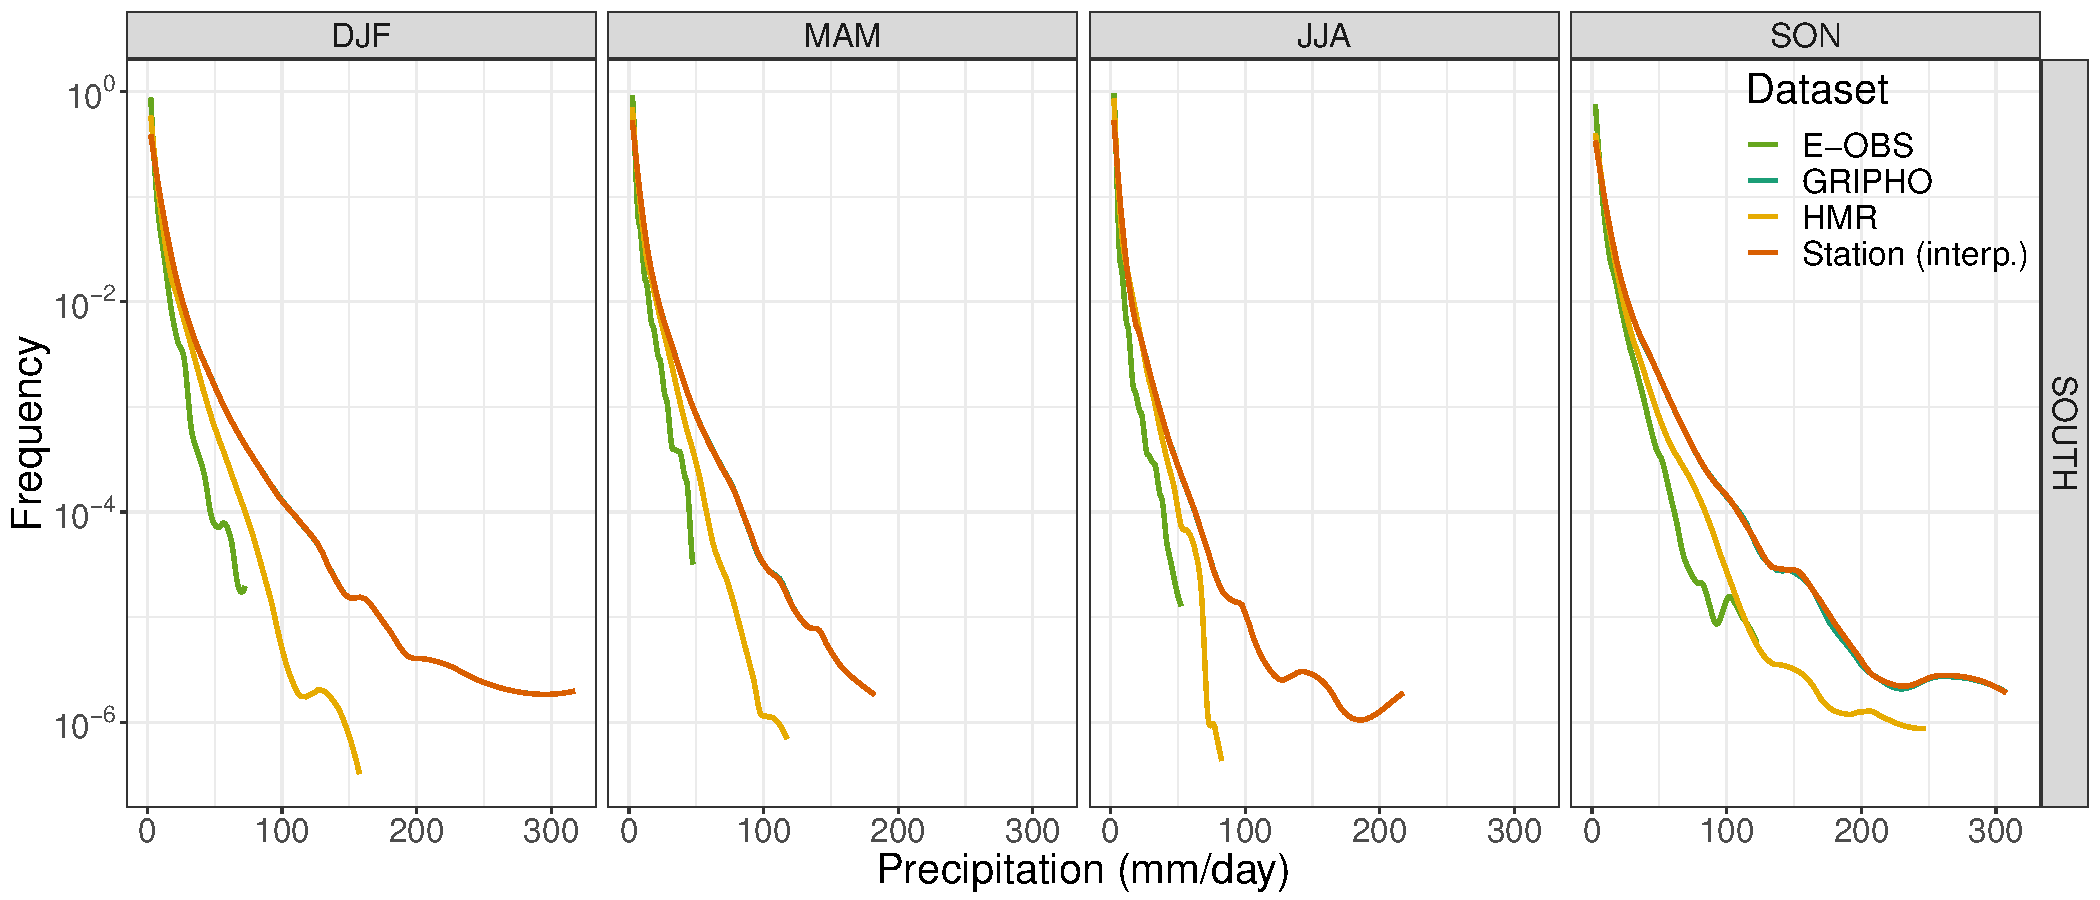
\includegraphics[width=0.8\textheight]{figures/valid_itaobs/pdf_SOUTH_lines}
        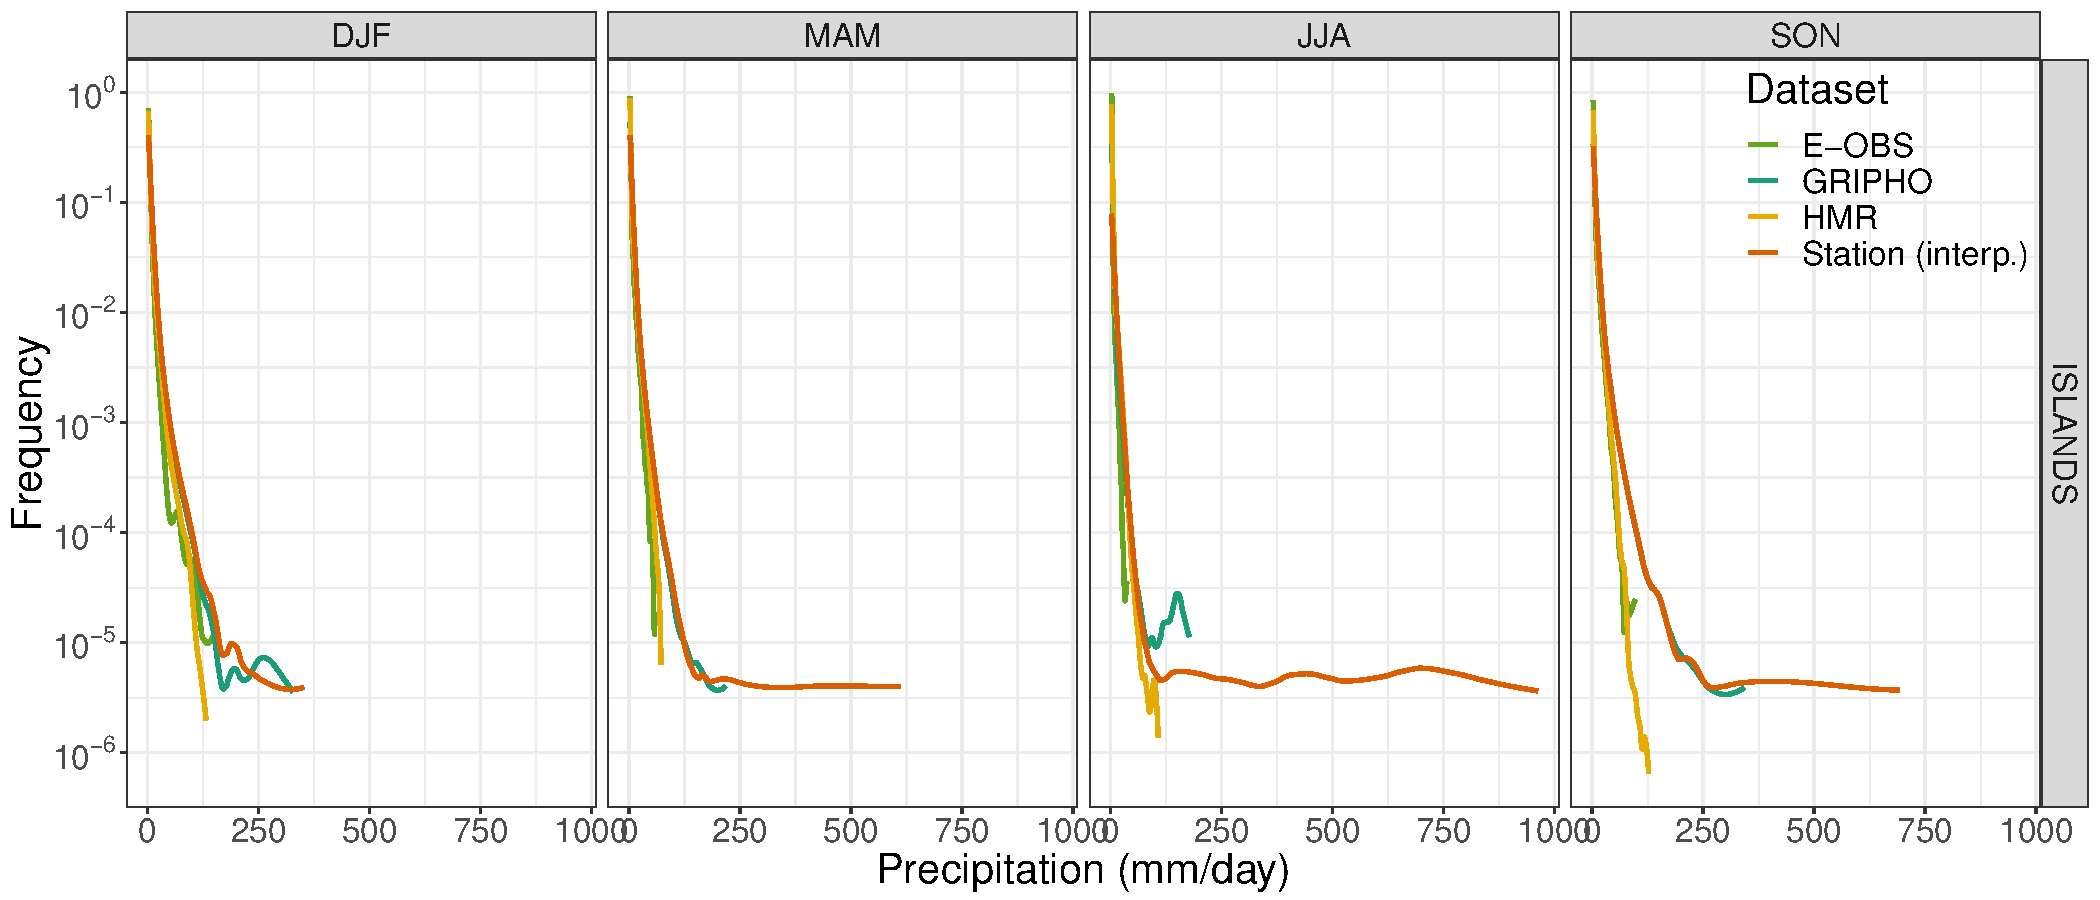
\includegraphics[width=0.8\textheight]{figures/valid_itaobs/pdf_ISLANDS_lines}
    \decoRule
    \caption[Validation of gridded hourly dataset: PDFs (2)]{
        Daily precipitation Probability Density Functions for the validation of the gridded hourly precipitation dataset for the South and Islands regions. The four summarising regions are highlighted in \cref{fig:valid_itaobs_pr_mean,fig:valid_itaobs_pr_r95}.
    }\label{fig:valid_itaobs_pr_pdf2}
\end{sidewaysfigure}

%------------------------------------
%	SUMMARY
%------------------------------------
\section{Summary and outlook}
The hourly precipitation dataset GRIPHO represents a first of its kind for the Italian territory.
The somewhat limited time availability of the dataset (little more than 15 years) is unfortunate, but no additional data was available for before 2000.
The high spatial and temporal resolution are superior to those of E-OBS, which is still the only observation-based dataset available over the whole Italian region. Compared to the ARCIS and EURO4M-APGD datasets, which are only available in Northern Italy, the effective spatial resolution is similar, but the hourly temporal resolution is much finer.
Thanks to the high station density, reproduction of extreme events is improved, in particular if compared to E-OBS.
The  GRIPHO dataset has shown sufficient quality for it to be used to drive the hydrological model CHyM, which is at the core of this thesis work, and to validate the climate simulations performed by RegCM, as detailed in the upcoming chapters.

Availability and additional details on this dataset will be made available in an upcoming paper \citep[][in preparation]{Fantini2018a}, where
\begin{itemize}
    \item the unexpected behaviour of extreme events in Sicily and Abruzzo will be fixed by applying a further manual conditioning step;
    \item an analysis of hourly precipitation will be included;
    \item the choice of interpolation method will be discussed further;
    \item validation against further datasets available for the area only on a monthly timescale (e.g. the ISAC/CNR dataset) will be included.
\end{itemize}
